\documentclass[twoside]{book}

% Packages required by doxygen
\usepackage{fixltx2e}
\usepackage{calc}
\usepackage{doxygen}
\usepackage[export]{adjustbox} % also loads graphicx
\usepackage{graphicx}
\usepackage[utf8]{inputenc}
\usepackage{makeidx}
\usepackage{multicol}
\usepackage{multirow}
\PassOptionsToPackage{warn}{textcomp}
\usepackage{textcomp}
\usepackage[nointegrals]{wasysym}
\usepackage[table]{xcolor}

% Font selection
\usepackage[T1]{fontenc}
\usepackage[scaled=.90]{helvet}
\usepackage{courier}
\usepackage{amssymb}
\usepackage{sectsty}
\renewcommand{\familydefault}{\sfdefault}
\allsectionsfont{%
  \fontseries{bc}\selectfont%
  \color{darkgray}%
}
\renewcommand{\DoxyLabelFont}{%
  \fontseries{bc}\selectfont%
  \color{darkgray}%
}
\newcommand{\+}{\discretionary{\mbox{\scriptsize$\hookleftarrow$}}{}{}}

% Page & text layout
\usepackage{geometry}
\geometry{%
  a4paper,%
  top=2.5cm,%
  bottom=2.5cm,%
  left=2.5cm,%
  right=2.5cm%
}
\tolerance=750
\hfuzz=15pt
\hbadness=750
\setlength{\emergencystretch}{15pt}
\setlength{\parindent}{0cm}
\setlength{\parskip}{3ex plus 2ex minus 2ex}
\makeatletter
\renewcommand{\paragraph}{%
  \@startsection{paragraph}{4}{0ex}{-1.0ex}{1.0ex}{%
    \normalfont\normalsize\bfseries\SS@parafont%
  }%
}
\renewcommand{\subparagraph}{%
  \@startsection{subparagraph}{5}{0ex}{-1.0ex}{1.0ex}{%
    \normalfont\normalsize\bfseries\SS@subparafont%
  }%
}
\makeatother

% Headers & footers
\usepackage{fancyhdr}
\pagestyle{fancyplain}
\fancyhead[LE]{\fancyplain{}{\bfseries\thepage}}
\fancyhead[CE]{\fancyplain{}{}}
\fancyhead[RE]{\fancyplain{}{\bfseries\leftmark}}
\fancyhead[LO]{\fancyplain{}{\bfseries\rightmark}}
\fancyhead[CO]{\fancyplain{}{}}
\fancyhead[RO]{\fancyplain{}{\bfseries\thepage}}
\fancyfoot[LE]{\fancyplain{}{}}
\fancyfoot[CE]{\fancyplain{}{}}
\fancyfoot[RE]{\fancyplain{}{\bfseries\scriptsize Generated by Doxygen }}
\fancyfoot[LO]{\fancyplain{}{\bfseries\scriptsize Generated by Doxygen }}
\fancyfoot[CO]{\fancyplain{}{}}
\fancyfoot[RO]{\fancyplain{}{}}
\renewcommand{\footrulewidth}{0.4pt}
\renewcommand{\chaptermark}[1]{%
  \markboth{#1}{}%
}
\renewcommand{\sectionmark}[1]{%
  \markright{\thesection\ #1}%
}

% Indices & bibliography
\usepackage{natbib}
\usepackage[titles]{tocloft}
\setcounter{tocdepth}{3}
\setcounter{secnumdepth}{5}
\makeindex

% Hyperlinks (required, but should be loaded last)
\usepackage{ifpdf}
\ifpdf
  \usepackage[pdftex,pagebackref=true]{hyperref}
\else
  \usepackage[ps2pdf,pagebackref=true]{hyperref}
\fi
\hypersetup{%
  colorlinks=true,%
  linkcolor=blue,%
  citecolor=blue,%
  unicode%
}

% Custom commands
\newcommand{\clearemptydoublepage}{%
  \newpage{\pagestyle{empty}\cleardoublepage}%
}

\usepackage{caption}
\captionsetup{labelsep=space,justification=centering,font={bf},singlelinecheck=off,skip=4pt,position=top}

%===== C O N T E N T S =====

\begin{document}

% Titlepage & ToC
\hypersetup{pageanchor=false,
             bookmarksnumbered=true,
             pdfencoding=unicode
            }
\pagenumbering{alph}
\begin{titlepage}
\vspace*{7cm}
\begin{center}%
{\Large Forex }\\
\vspace*{1cm}
{\large Generated by Doxygen 1.8.12}\\
\end{center}
\end{titlepage}
\clearemptydoublepage
\pagenumbering{roman}
\tableofcontents
\clearemptydoublepage
\pagenumbering{arabic}
\hypersetup{pageanchor=true}

%--- Begin generated contents ---
\chapter{Namespace Index}
\section{Namespace List}
Here is a list of all documented namespaces with brief descriptions\+:\begin{DoxyCompactList}
\item\contentsline{section}{\hyperlink{namespace_client}{Client} }{\pageref{namespace_client}}{}
\end{DoxyCompactList}

\chapter{Hierarchical Index}
\section{Class Hierarchy}
This inheritance list is sorted roughly, but not completely, alphabetically\+:\begin{DoxyCompactList}
\item \contentsline{section}{Client.\+Bd}{\pageref{class_client_1_1_bd}}{}
\begin{DoxyCompactList}
\item \contentsline{section}{Client.\+Bd\+Reqest}{\pageref{class_client_1_1_bd_reqest}}{}
\end{DoxyCompactList}
\item Button\begin{DoxyCompactList}
\item \contentsline{section}{Client.\+Extend\+Button}{\pageref{class_client_1_1_extend_button}}{}
\end{DoxyCompactList}
\item \contentsline{section}{Client.\+ChartQ}{\pageref{class_client_1_1_chart_q}}{}
\item Check\+Box\begin{DoxyCompactList}
\item \contentsline{section}{Client.\+Extend\+Checkbox}{\pageref{class_client_1_1_extend_checkbox}}{}
\end{DoxyCompactList}
\item \contentsline{section}{Client.\+Class\+S\+MA}{\pageref{class_client_1_1_class_s_m_a}}{}
\item \contentsline{section}{Client.\+Deal}{\pageref{class_client_1_1_deal}}{}
\item \contentsline{section}{Client.\+Directory\+Work}{\pageref{class_client_1_1_directory_work}}{}
\item \contentsline{section}{Client.\+Display}{\pageref{class_client_1_1_display}}{}
\item \contentsline{section}{Client.\+Event}{\pageref{class_client_1_1_event}}{}
\item \contentsline{section}{Client.\+Exel}{\pageref{class_client_1_1_exel}}{}
\item \contentsline{section}{Client.\+File\+Inspection}{\pageref{class_client_1_1_file_inspection}}{}
\begin{DoxyCompactList}
\item \contentsline{section}{Client.\+Work\+File}{\pageref{class_client_1_1_work_file}}{}
\end{DoxyCompactList}
\item Form\begin{DoxyCompactList}
\item \contentsline{section}{Client.\+Close\+Deal}{\pageref{class_client_1_1_close_deal}}{}
\item \contentsline{section}{Client.\+Help}{\pageref{class_client_1_1_help}}{}
\item \contentsline{section}{Client.\+Main\+Form}{\pageref{class_client_1_1_main_form}}{}
\item \contentsline{section}{Client.\+Report}{\pageref{class_client_1_1_report}}{}
\item \contentsline{section}{Client.\+Setting}{\pageref{class_client_1_1_setting}}{}
\item \contentsline{section}{Client.\+S\+Window}{\pageref{class_client_1_1_s_window}}{}
\item \contentsline{section}{Client.\+Windowd}{\pageref{class_client_1_1_windowd}}{}
\end{DoxyCompactList}
\item \contentsline{section}{Client.\+GraphY}{\pageref{class_client_1_1_graph_y}}{}
\item \contentsline{section}{Client.\+Interface}{\pageref{interface_client_1_1_interface}}{}
\item \contentsline{section}{Client.\+Internet}{\pageref{class_client_1_1_internet}}{}
\begin{DoxyCompactList}
\item \contentsline{section}{Client.\+Internet\+Request}{\pageref{class_client_1_1_internet_request}}{}
\end{DoxyCompactList}
\item \contentsline{section}{Client.\+Interval\+Resistance}{\pageref{class_client_1_1_interval_resistance}}{}
\item Label\begin{DoxyCompactList}
\item \contentsline{section}{Client.\+Extend\+Label}{\pageref{class_client_1_1_extend_label}}{}
\end{DoxyCompactList}
\item \contentsline{section}{Client.\+Line\+Coord}{\pageref{class_client_1_1_line_coord}}{}
\item \contentsline{section}{Client.\+Methods}{\pageref{class_client_1_1_methods}}{}
\item \contentsline{section}{Client.\+Min\+Max}{\pageref{class_client_1_1_min_max}}{}
\item \contentsline{section}{Client.\+Parser}{\pageref{class_client_1_1_parser}}{}
\item \contentsline{section}{Client.\+Quotes}{\pageref{class_client_1_1_quotes}}{}
\item \contentsline{section}{Client.\+Resistance}{\pageref{class_client_1_1_resistance}}{}
\item \contentsline{section}{Client.\+Splice}{\pageref{class_client_1_1_splice}}{}
\item \contentsline{section}{Client.\+Support}{\pageref{class_client_1_1_support}}{}
\item Tool\+Strip\+Menu\+Item\begin{DoxyCompactList}
\item \contentsline{section}{Client.\+Extend\+Tool\+Strip\+Menu\+Item}{\pageref{class_client_1_1_extend_tool_strip_menu_item}}{}
\end{DoxyCompactList}
\item User\+Control\begin{DoxyCompactList}
\item \contentsline{section}{Client.\+buttonL}{\pageref{class_client_1_1button_l}}{}
\end{DoxyCompactList}
\item \contentsline{section}{Client.\+window\+Quotes}{\pageref{class_client_1_1window_quotes}}{}
\item \contentsline{section}{Client.\+ZoomS}{\pageref{class_client_1_1_zoom_s}}{}
\end{DoxyCompactList}

\chapter{Class Index}
\section{Class List}
Here are the classes, structs, unions and interfaces with brief descriptions\+:\begin{DoxyCompactList}
\item\contentsline{section}{\hyperlink{class_client_1_1_bd}{Client.\+Bd} \\*Класс базы данных }{\pageref{class_client_1_1_bd}}{}
\item\contentsline{section}{\hyperlink{class_client_1_1_bd_reqest}{Client.\+Bd\+Reqest} \\*Класс для работы с объектом база данных }{\pageref{class_client_1_1_bd_reqest}}{}
\item\contentsline{section}{\hyperlink{class_client_1_1button_l}{Client.\+buttonL} }{\pageref{class_client_1_1button_l}}{}
\item\contentsline{section}{\hyperlink{class_client_1_1_chart_q}{Client.\+ChartQ} \\*Класс для изменения чарта и задание линий }{\pageref{class_client_1_1_chart_q}}{}
\item\contentsline{section}{\hyperlink{class_client_1_1_class_s_m_a}{Client.\+Class\+S\+MA} \\*Вычисление линии S\+MA + }{\pageref{class_client_1_1_class_s_m_a}}{}
\item\contentsline{section}{\hyperlink{class_client_1_1_close_deal}{Client.\+Close\+Deal} \\*Класс по закрытию сделки }{\pageref{class_client_1_1_close_deal}}{}
\item\contentsline{section}{\hyperlink{class_client_1_1_deal}{Client.\+Deal} \\*Класс сохраняющий сделки }{\pageref{class_client_1_1_deal}}{}
\item\contentsline{section}{\hyperlink{class_client_1_1_directory_work}{Client.\+Directory\+Work} \\*Класс для работы с директорией }{\pageref{class_client_1_1_directory_work}}{}
\item\contentsline{section}{\hyperlink{class_client_1_1_display}{Client.\+Display} \\*Класс для адаптации размеров окон под размеры экрана }{\pageref{class_client_1_1_display}}{}
\item\contentsline{section}{\hyperlink{class_client_1_1_event}{Client.\+Event} \\*Событие }{\pageref{class_client_1_1_event}}{}
\item\contentsline{section}{\hyperlink{class_client_1_1_exel}{Client.\+Exel} \\*Класс отвечающий за работу с \hyperlink{class_client_1_1_exel}{Exel} }{\pageref{class_client_1_1_exel}}{}
\item\contentsline{section}{\hyperlink{class_client_1_1_extend_button}{Client.\+Extend\+Button} \\*Класс расширяюший базовые возможности кнопки }{\pageref{class_client_1_1_extend_button}}{}
\item\contentsline{section}{\hyperlink{class_client_1_1_extend_checkbox}{Client.\+Extend\+Checkbox} \\*Класс расширяюший базовые возможности чекбокс }{\pageref{class_client_1_1_extend_checkbox}}{}
\item\contentsline{section}{\hyperlink{class_client_1_1_extend_label}{Client.\+Extend\+Label} \\*Класс расширяюший базовые возможности лабел }{\pageref{class_client_1_1_extend_label}}{}
\item\contentsline{section}{\hyperlink{class_client_1_1_extend_tool_strip_menu_item}{Client.\+Extend\+Tool\+Strip\+Menu\+Item} \\*Класс расширяюший базовые возможности меню }{\pageref{class_client_1_1_extend_tool_strip_menu_item}}{}
\item\contentsline{section}{\hyperlink{class_client_1_1_file_inspection}{Client.\+File\+Inspection} \\*Классд для проверки существования файла }{\pageref{class_client_1_1_file_inspection}}{}
\item\contentsline{section}{\hyperlink{class_client_1_1_graph_y}{Client.\+GraphY} \\*класс отвечающий за диапазон графика }{\pageref{class_client_1_1_graph_y}}{}
\item\contentsline{section}{\hyperlink{class_client_1_1_help}{Client.\+Help} \\*Класс отвечающий за окно \hyperlink{class_client_1_1_help}{Help} }{\pageref{class_client_1_1_help}}{}
\item\contentsline{section}{\hyperlink{interface_client_1_1_interface}{Client.\+Interface} \\*Интерфейс }{\pageref{interface_client_1_1_interface}}{}
\item\contentsline{section}{\hyperlink{class_client_1_1_internet}{Client.\+Internet} \\*Класс отечающий за работу с интернетом }{\pageref{class_client_1_1_internet}}{}
\item\contentsline{section}{\hyperlink{class_client_1_1_internet_request}{Client.\+Internet\+Request} \\*Класс интернет запрос }{\pageref{class_client_1_1_internet_request}}{}
\item\contentsline{section}{\hyperlink{class_client_1_1_interval_resistance}{Client.\+Interval\+Resistance} \\*Класс формирующий интервалы линии сопротивления }{\pageref{class_client_1_1_interval_resistance}}{}
\item\contentsline{section}{\hyperlink{class_client_1_1_line_coord}{Client.\+Line\+Coord} \\*Класс отвечающий за координатные линии }{\pageref{class_client_1_1_line_coord}}{}
\item\contentsline{section}{\hyperlink{class_client_1_1_main_form}{Client.\+Main\+Form} \\*Стартовое окно }{\pageref{class_client_1_1_main_form}}{}
\item\contentsline{section}{\hyperlink{class_client_1_1_methods}{Client.\+Methods} \\*Class \hyperlink{class_client_1_1_methods}{Methods} }{\pageref{class_client_1_1_methods}}{}
\item\contentsline{section}{\hyperlink{class_client_1_1_min_max}{Client.\+Min\+Max} \\*Класс минимум максимум }{\pageref{class_client_1_1_min_max}}{}
\item\contentsline{section}{\hyperlink{class_client_1_1_parser}{Client.\+Parser} \\*Парсер данных }{\pageref{class_client_1_1_parser}}{}
\item\contentsline{section}{\hyperlink{class_client_1_1_quotes}{Client.\+Quotes} \\*Класс котировка }{\pageref{class_client_1_1_quotes}}{}
\item\contentsline{section}{\hyperlink{class_client_1_1_report}{Client.\+Report} \\*Класс отвечающий за формирование отчета }{\pageref{class_client_1_1_report}}{}
\item\contentsline{section}{\hyperlink{class_client_1_1_resistance}{Client.\+Resistance} \\*Класс отвечающий за сущность линии сопротивления }{\pageref{class_client_1_1_resistance}}{}
\item\contentsline{section}{\hyperlink{class_client_1_1_setting}{Client.\+Setting} \\*Класс для задания размеров окнаы }{\pageref{class_client_1_1_setting}}{}
\item\contentsline{section}{\hyperlink{class_client_1_1_splice}{Client.\+Splice} \\*Класс соединяющий буферные значения с файловыми }{\pageref{class_client_1_1_splice}}{}
\item\contentsline{section}{\hyperlink{class_client_1_1_support}{Client.\+Support} \\*класс отвечает за создание сущности линии поддержки }{\pageref{class_client_1_1_support}}{}
\item\contentsline{section}{\hyperlink{class_client_1_1_s_window}{Client.\+S\+Window} \\*класс для задание размеров формы котировки }{\pageref{class_client_1_1_s_window}}{}
\item\contentsline{section}{\hyperlink{class_client_1_1_windowd}{Client.\+Windowd} \\*Форма для взаиможействия с графиками котировок и создания сделок }{\pageref{class_client_1_1_windowd}}{}
\item\contentsline{section}{\hyperlink{class_client_1_1window_quotes}{Client.\+window\+Quotes} \\*Класс парсинга котировок }{\pageref{class_client_1_1window_quotes}}{}
\item\contentsline{section}{\hyperlink{class_client_1_1_work_file}{Client.\+Work\+File} \\*Класс отвечающий за работу с файлами }{\pageref{class_client_1_1_work_file}}{}
\item\contentsline{section}{\hyperlink{class_client_1_1_zoom_s}{Client.\+ZoomS} \\*Класс для работы с масштабоом графика }{\pageref{class_client_1_1_zoom_s}}{}
\end{DoxyCompactList}

\chapter{Namespace Documentation}
\hypertarget{namespace_client}{}\section{Client Namespace Reference}
\label{namespace_client}\index{Client@{Client}}
\subsection*{Classes}
\begin{DoxyCompactItemize}
\item 
class {\bfseries Activ}
\item 
class \hyperlink{class_client_1_1_bd}{Bd}
\begin{DoxyCompactList}\small\item\em Класс базы данных \end{DoxyCompactList}\item 
class \hyperlink{class_client_1_1_bd_reqest}{Bd\+Reqest}
\begin{DoxyCompactList}\small\item\em Класс для работы с объектом база данных \end{DoxyCompactList}\item 
class \hyperlink{class_client_1_1button_l}{buttonL}
\item 
class \hyperlink{class_client_1_1_chart_q}{ChartQ}
\begin{DoxyCompactList}\small\item\em Класс для изменения чарта и задание линий \end{DoxyCompactList}\item 
class \hyperlink{class_client_1_1_class_s_m_a}{Class\+S\+MA}
\begin{DoxyCompactList}\small\item\em Вычисление линии S\+MA + \end{DoxyCompactList}\item 
class \hyperlink{class_client_1_1_close_deal}{Close\+Deal}
\begin{DoxyCompactList}\small\item\em Класс по закрытию сделки \end{DoxyCompactList}\item 
class \hyperlink{class_client_1_1_deal}{Deal}
\begin{DoxyCompactList}\small\item\em Класс сохраняющий сделки \end{DoxyCompactList}\item 
class \hyperlink{class_client_1_1_directory_work}{Directory\+Work}
\begin{DoxyCompactList}\small\item\em Класс для работы с директорией \end{DoxyCompactList}\item 
class \hyperlink{class_client_1_1_display}{Display}
\begin{DoxyCompactList}\small\item\em Класс для адаптации размеров окон под размеры экрана \end{DoxyCompactList}\item 
class \hyperlink{class_client_1_1_event}{Event}
\begin{DoxyCompactList}\small\item\em Событие \end{DoxyCompactList}\item 
class \hyperlink{class_client_1_1_exel}{Exel}
\begin{DoxyCompactList}\small\item\em Класс отвечающий за работу с \hyperlink{class_client_1_1_exel}{Exel} \end{DoxyCompactList}\item 
class \hyperlink{class_client_1_1_extend_button}{Extend\+Button}
\begin{DoxyCompactList}\small\item\em Класс расширяюший базовые возможности кнопки \end{DoxyCompactList}\item 
class \hyperlink{class_client_1_1_extend_checkbox}{Extend\+Checkbox}
\begin{DoxyCompactList}\small\item\em Класс расширяюший базовые возможности чекбокс \end{DoxyCompactList}\item 
class \hyperlink{class_client_1_1_extend_label}{Extend\+Label}
\begin{DoxyCompactList}\small\item\em Класс расширяюший базовые возможности лабел \end{DoxyCompactList}\item 
class \hyperlink{class_client_1_1_extend_tool_strip_menu_item}{Extend\+Tool\+Strip\+Menu\+Item}
\begin{DoxyCompactList}\small\item\em Класс расширяюший базовые возможности меню \end{DoxyCompactList}\item 
class \hyperlink{class_client_1_1_file_inspection}{File\+Inspection}
\begin{DoxyCompactList}\small\item\em Классд для проверки существования файла \end{DoxyCompactList}\item 
class \hyperlink{class_client_1_1_graph_y}{GraphY}
\begin{DoxyCompactList}\small\item\em класс отвечающий за диапазон графика \end{DoxyCompactList}\item 
class \hyperlink{class_client_1_1_help}{Help}
\begin{DoxyCompactList}\small\item\em Класс отвечающий за окно \hyperlink{class_client_1_1_help}{Help} \end{DoxyCompactList}\item 
class {\bfseries Inet\+Connect}
\item 
interface \hyperlink{interface_client_1_1_interface}{Interface}
\begin{DoxyCompactList}\small\item\em Интерфейс \end{DoxyCompactList}\item 
class \hyperlink{class_client_1_1_internet}{Internet}
\begin{DoxyCompactList}\small\item\em Класс отечающий за работу с интернетом \end{DoxyCompactList}\item 
class \hyperlink{class_client_1_1_internet_request}{Internet\+Request}
\begin{DoxyCompactList}\small\item\em Класс интернет запрос \end{DoxyCompactList}\item 
class \hyperlink{class_client_1_1_interval_resistance}{Interval\+Resistance}
\begin{DoxyCompactList}\small\item\em Класс формирующий интервалы линии сопротивления \end{DoxyCompactList}\item 
class \hyperlink{class_client_1_1_line_coord}{Line\+Coord}
\begin{DoxyCompactList}\small\item\em Класс отвечающий за координатные линии \end{DoxyCompactList}\item 
class \hyperlink{class_client_1_1_main_form}{Main\+Form}
\begin{DoxyCompactList}\small\item\em Стартовое окно \end{DoxyCompactList}\item 
class \hyperlink{class_client_1_1_methods}{Methods}
\begin{DoxyCompactList}\small\item\em Class \hyperlink{class_client_1_1_methods}{Methods} \end{DoxyCompactList}\item 
class \hyperlink{class_client_1_1_min_max}{Min\+Max}
\begin{DoxyCompactList}\small\item\em Класс минимум максимум \end{DoxyCompactList}\item 
class \hyperlink{class_client_1_1_parser}{Parser}
\begin{DoxyCompactList}\small\item\em Парсер данных \end{DoxyCompactList}\item 
class {\bfseries Program}
\item 
class \hyperlink{class_client_1_1_quotes}{Quotes}
\begin{DoxyCompactList}\small\item\em Класс котировка \end{DoxyCompactList}\item 
class \hyperlink{class_client_1_1_report}{Report}
\begin{DoxyCompactList}\small\item\em Класс отвечающий за формирование отчета \end{DoxyCompactList}\item 
class {\bfseries Report\+Transit}
\item 
class \hyperlink{class_client_1_1_resistance}{Resistance}
\begin{DoxyCompactList}\small\item\em Класс отвечающий за сущность линии сопротивления \end{DoxyCompactList}\item 
class \hyperlink{class_client_1_1_setting}{Setting}
\begin{DoxyCompactList}\small\item\em Класс для задания размеров окнаы \end{DoxyCompactList}\item 
class {\bfseries Speed\+Draw}
\item 
class \hyperlink{class_client_1_1_splice}{Splice}
\begin{DoxyCompactList}\small\item\em Класс соединяющий буферные значения с файловыми \end{DoxyCompactList}\item 
class \hyperlink{class_client_1_1_support}{Support}
\begin{DoxyCompactList}\small\item\em класс отвечает за создание сущности линии поддержки \end{DoxyCompactList}\item 
class \hyperlink{class_client_1_1_s_window}{S\+Window}
\begin{DoxyCompactList}\small\item\em класс для задание размеров формы котировки \end{DoxyCompactList}\item 
class \hyperlink{class_client_1_1_windowd}{Windowd}
\begin{DoxyCompactList}\small\item\em Форма для взаиможействия с графиками котировок и создания сделок \end{DoxyCompactList}\item 
class \hyperlink{class_client_1_1window_quotes}{window\+Quotes}
\begin{DoxyCompactList}\small\item\em Класс парсинга котировок \end{DoxyCompactList}\item 
class \hyperlink{class_client_1_1_work_file}{Work\+File}
\begin{DoxyCompactList}\small\item\em Класс отвечающий за работу с файлами \end{DoxyCompactList}\item 
class {\bfseries W\+String}
\item 
class \hyperlink{class_client_1_1_zoom_s}{ZoomS}
\begin{DoxyCompactList}\small\item\em Класс для работы с масштабоом графика \end{DoxyCompactList}\end{DoxyCompactItemize}
\subsection*{Typedefs}
\begin{DoxyCompactItemize}
\item 
\hypertarget{namespace_client_ae20e76d5488b468826600e98538df2a3}{}\label{namespace_client_ae20e76d5488b468826600e98538df2a3} 
using {\bfseries Enum\+Dialog\+Result} = System.\+Windows.\+Forms.\+Dialog\+Result
\item 
\hypertarget{namespace_client_aec74278014a479f235b75f6c96cb7529}{}\label{namespace_client_aec74278014a479f235b75f6c96cb7529} 
using {\bfseries Excel} = Microsoft.\+Office.\+Interop.\+Excel
\end{DoxyCompactItemize}

\chapter{Class Documentation}
\hypertarget{class_client_1_1_bd}{}\section{Client.\+Bd Class Reference}
\label{class_client_1_1_bd}\index{Client.\+Bd@{Client.\+Bd}}


Класс базы данных  


Inheritance diagram for Client.\+Bd\+:\begin{figure}[H]
\begin{center}
\leavevmode
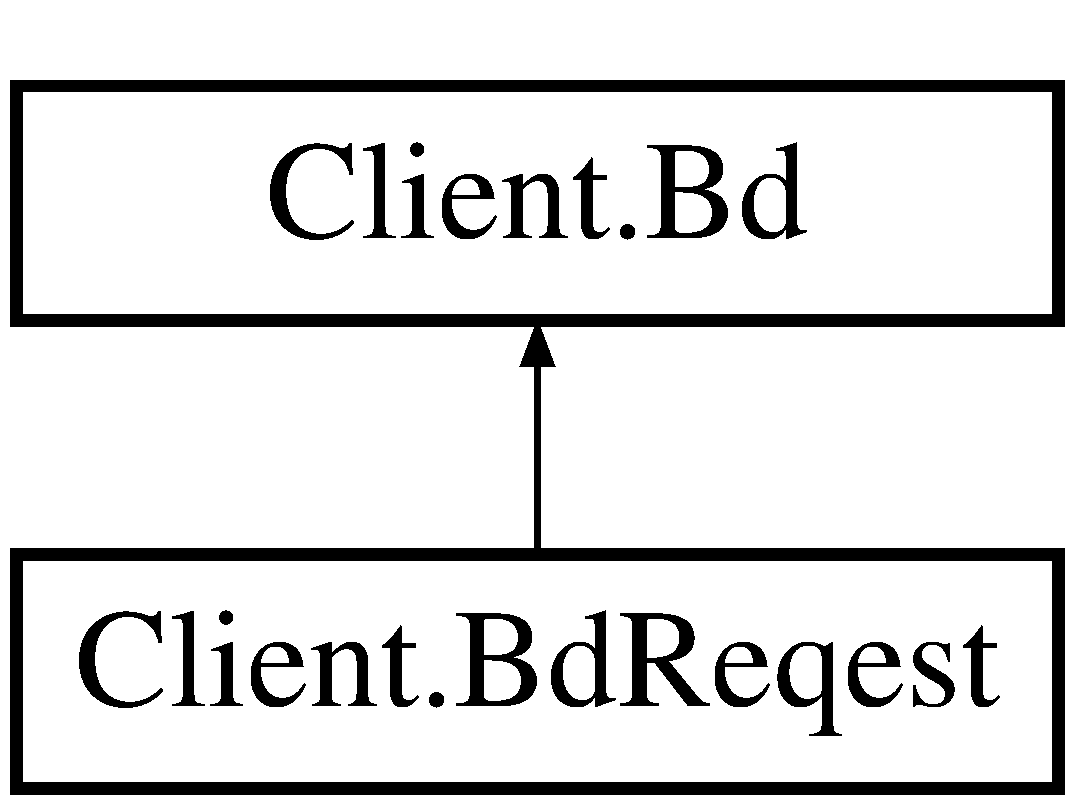
\includegraphics[height=2.000000cm]{class_client_1_1_bd}
\end{center}
\end{figure}
\subsection*{Public Member Functions}
\begin{DoxyCompactItemize}
\item 
\hyperlink{class_client_1_1_bd_a66346f172528dd64f567b7687afb1a33}{Bd} (string \+\_\+patch)
\begin{DoxyCompactList}\small\item\em данные конфигурации \end{DoxyCompactList}\item 
void \hyperlink{class_client_1_1_bd_ad4e3f2477942897e846e3cf247419518}{bd\+Load} (string bd\+Value, int number)
\begin{DoxyCompactList}\small\item\em загрузка в бд \end{DoxyCompactList}\item 
Task \hyperlink{class_client_1_1_bd_a39c09d734ca537c31b51af1f0a3ef84c}{Load\+Data} (string value)
\begin{DoxyCompactList}\small\item\em Метод загрузки данных \end{DoxyCompactList}\item 
string \hyperlink{class_client_1_1_bd_a1127b7b1b53edf9e1b86c4292a1e91cd}{Task\+Connect} (string value)
\begin{DoxyCompactList}\small\item\em Метод загрузки данных + \end{DoxyCompactList}\item 
\hypertarget{class_client_1_1_bd_ad831f343ca4a5ea39a875c6f52eeeb78}{}\label{class_client_1_1_bd_ad831f343ca4a5ea39a875c6f52eeeb78} 
string {\bfseries get\+Patch} ()
\end{DoxyCompactItemize}
\subsection*{Protected Attributes}
\begin{DoxyCompactItemize}
\item 
string \hyperlink{class_client_1_1_bd_a4fff732ae82883ee9238243620430c41}{patch}
\begin{DoxyCompactList}\small\item\em путь \end{DoxyCompactList}\end{DoxyCompactItemize}


\subsection{Detailed Description}
Класс базы данных 



\subsection{Constructor \& Destructor Documentation}
\hypertarget{class_client_1_1_bd_a66346f172528dd64f567b7687afb1a33}{}\label{class_client_1_1_bd_a66346f172528dd64f567b7687afb1a33} 
\index{Client\+::\+Bd@{Client\+::\+Bd}!Bd@{Bd}}
\index{Bd@{Bd}!Client\+::\+Bd@{Client\+::\+Bd}}
\subsubsection{\texorpdfstring{Bd()}{Bd()}}
{\footnotesize\ttfamily Client.\+Bd.\+Bd (\begin{DoxyParamCaption}\item[{string}]{\+\_\+patch }\end{DoxyParamCaption})\hspace{0.3cm}{\ttfamily [inline]}}



данные конфигурации 


\begin{DoxyParams}{Parameters}
{\em \+\_\+patch} & Путь/param$>$ \\
\hline
\end{DoxyParams}


\subsection{Member Function Documentation}
\hypertarget{class_client_1_1_bd_ad4e3f2477942897e846e3cf247419518}{}\label{class_client_1_1_bd_ad4e3f2477942897e846e3cf247419518} 
\index{Client\+::\+Bd@{Client\+::\+Bd}!bd\+Load@{bd\+Load}}
\index{bd\+Load@{bd\+Load}!Client\+::\+Bd@{Client\+::\+Bd}}
\subsubsection{\texorpdfstring{bd\+Load()}{bdLoad()}}
{\footnotesize\ttfamily void Client.\+Bd.\+bd\+Load (\begin{DoxyParamCaption}\item[{string}]{bd\+Value,  }\item[{int}]{number }\end{DoxyParamCaption})\hspace{0.3cm}{\ttfamily [inline]}}



загрузка в бд 


\begin{DoxyParams}{Parameters}
{\em bd\+Value} & Котировка/param$>$ 
\begin{DoxyParams}{Parameters}
{\em number} & Кол-\/во/param$>$ \\
\hline
\end{DoxyParams}
\\
\hline
\end{DoxyParams}
\hypertarget{class_client_1_1_bd_a39c09d734ca537c31b51af1f0a3ef84c}{}\label{class_client_1_1_bd_a39c09d734ca537c31b51af1f0a3ef84c} 
\index{Client\+::\+Bd@{Client\+::\+Bd}!Load\+Data@{Load\+Data}}
\index{Load\+Data@{Load\+Data}!Client\+::\+Bd@{Client\+::\+Bd}}
\subsubsection{\texorpdfstring{Load\+Data()}{LoadData()}}
{\footnotesize\ttfamily Task Client.\+Bd.\+Load\+Data (\begin{DoxyParamCaption}\item[{string}]{value }\end{DoxyParamCaption})\hspace{0.3cm}{\ttfamily [inline]}}



Метод загрузки данных 


\begin{DoxyParams}{Parameters}
{\em Basa\+Dan} & База данных\\
\hline
{\em value} & Котировка\\
\hline
\end{DoxyParams}
\hypertarget{class_client_1_1_bd_a1127b7b1b53edf9e1b86c4292a1e91cd}{}\label{class_client_1_1_bd_a1127b7b1b53edf9e1b86c4292a1e91cd} 
\index{Client\+::\+Bd@{Client\+::\+Bd}!Task\+Connect@{Task\+Connect}}
\index{Task\+Connect@{Task\+Connect}!Client\+::\+Bd@{Client\+::\+Bd}}
\subsubsection{\texorpdfstring{Task\+Connect()}{TaskConnect()}}
{\footnotesize\ttfamily string Client.\+Bd.\+Task\+Connect (\begin{DoxyParamCaption}\item[{string}]{value }\end{DoxyParamCaption})\hspace{0.3cm}{\ttfamily [inline]}}



Метод загрузки данных + 


\begin{DoxyParams}{Parameters}
{\em value} & Котировка\\
\hline
\end{DoxyParams}


\subsection{Member Data Documentation}
\hypertarget{class_client_1_1_bd_a4fff732ae82883ee9238243620430c41}{}\label{class_client_1_1_bd_a4fff732ae82883ee9238243620430c41} 
\index{Client\+::\+Bd@{Client\+::\+Bd}!patch@{patch}}
\index{patch@{patch}!Client\+::\+Bd@{Client\+::\+Bd}}
\subsubsection{\texorpdfstring{patch}{patch}}
{\footnotesize\ttfamily string Client.\+Bd.\+patch\hspace{0.3cm}{\ttfamily [protected]}}



путь 



The documentation for this class was generated from the following file\+:\begin{DoxyCompactItemize}
\item 
C\+:/\+Users/саша/\+Documents/\+Visual Studio 2015/\+Projects/\+Forex2.\+0/\+Client/Bd.\+cs\end{DoxyCompactItemize}

\hypertarget{class_client_1_1_bd_reqest}{}\section{Client.\+Bd\+Reqest Class Reference}
\label{class_client_1_1_bd_reqest}\index{Client.\+Bd\+Reqest@{Client.\+Bd\+Reqest}}


Класс для работы с объектом база данных  


Inheritance diagram for Client.\+Bd\+Reqest\+:\begin{figure}[H]
\begin{center}
\leavevmode
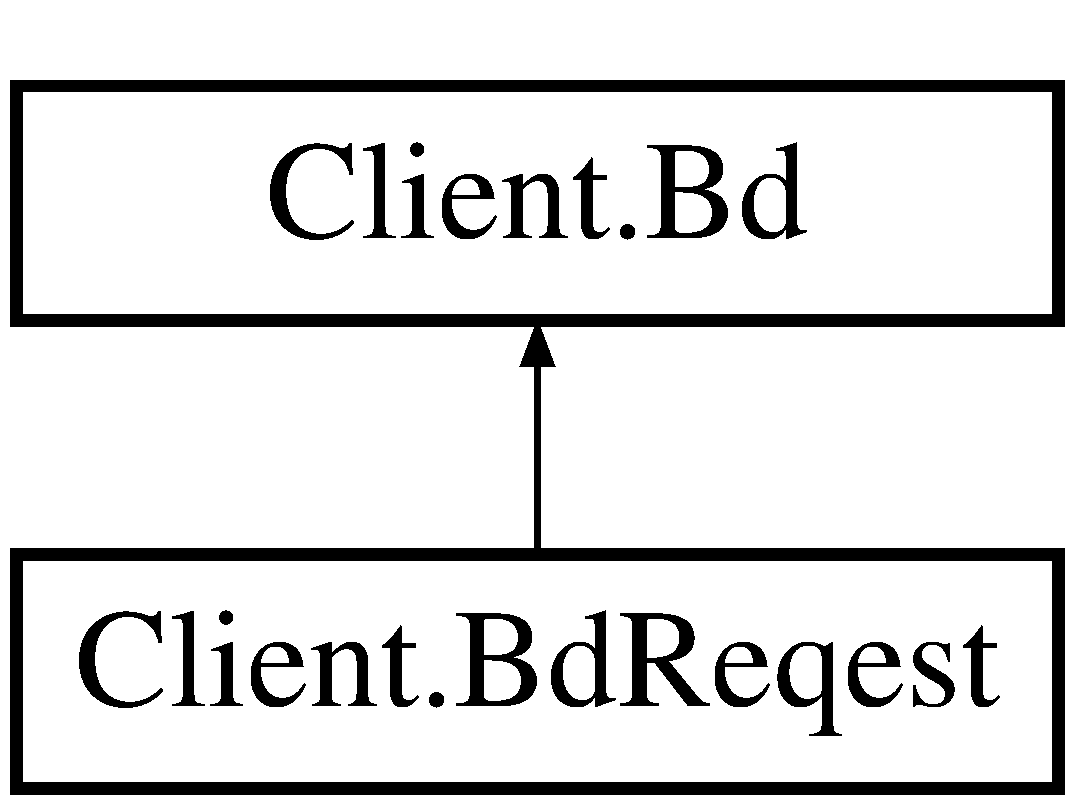
\includegraphics[height=2.000000cm]{class_client_1_1_bd_reqest}
\end{center}
\end{figure}
\subsection*{Public Member Functions}
\begin{DoxyCompactItemize}
\item 
\hyperlink{class_client_1_1_bd_reqest_a782e678c91671039896a90ac999b8966}{Bd\+Reqest} (string \+\_\+patch)
\begin{DoxyCompactList}\small\item\em Конструктор запросов для объекта БД \end{DoxyCompactList}\item 
void \hyperlink{class_client_1_1_bd_reqest_ab782415f646f42b5c4e64b74d68d0bcf}{Command\+Select} (ref List$<$ int $>$ ListT, ref List$<$ double $>$ ListB, ref List$<$ double $>$ ListS, string Value, Sql\+Connection con)
\begin{DoxyCompactList}\small\item\em Запрос на извлечение данных \end{DoxyCompactList}\item 
void \hyperlink{class_client_1_1_bd_reqest_ad9b512bdcefe04563e937ab9edb0864d}{Command\+Select} (ref List$<$ int $>$ ListT, string Value, Sql\+Connection con)
\begin{DoxyCompactList}\small\item\em Запрос последнего времени из бд \end{DoxyCompactList}\item 
int \hyperlink{class_client_1_1_bd_reqest_ac978622ddc77c5198af52e5fccefdcc2}{last\+Time} (string Value, Sql\+Connection con)
\begin{DoxyCompactList}\small\item\em Запрос последнего времени из бд \end{DoxyCompactList}\item 
void \hyperlink{class_client_1_1_bd_reqest_ae9e0d4839d82d8e9573d867d9dfd8755}{Insert} (string Value, List$<$ int $>$ Time, List$<$ double $>$ Buy, List$<$ double $>$ Sell, Sql\+Connection con)
\begin{DoxyCompactList}\small\item\em Запрос на добавлени данных \end{DoxyCompactList}\item 
void \hyperlink{class_client_1_1_bd_reqest_aa429c52005707d06a7df660f3dc6eb62}{form\+Insert} (int Time, double Bid, double Ask, string Value, Sql\+Connection con)
\begin{DoxyCompactList}\small\item\em Запрос на добавлени данных \end{DoxyCompactList}\end{DoxyCompactItemize}
\subsection*{Additional Inherited Members}


\subsection{Detailed Description}
Класс для работы с объектом база данных 



\subsection{Constructor \& Destructor Documentation}
\hypertarget{class_client_1_1_bd_reqest_a782e678c91671039896a90ac999b8966}{}\label{class_client_1_1_bd_reqest_a782e678c91671039896a90ac999b8966} 
\index{Client\+::\+Bd\+Reqest@{Client\+::\+Bd\+Reqest}!Bd\+Reqest@{Bd\+Reqest}}
\index{Bd\+Reqest@{Bd\+Reqest}!Client\+::\+Bd\+Reqest@{Client\+::\+Bd\+Reqest}}
\subsubsection{\texorpdfstring{Bd\+Reqest()}{BdReqest()}}
{\footnotesize\ttfamily Client.\+Bd\+Reqest.\+Bd\+Reqest (\begin{DoxyParamCaption}\item[{string}]{\+\_\+patch }\end{DoxyParamCaption})\hspace{0.3cm}{\ttfamily [inline]}}



Конструктор запросов для объекта БД 


\begin{DoxyParams}{Parameters}
{\em \+\_\+patch} & Путь к БД\\
\hline
\end{DoxyParams}


\subsection{Member Function Documentation}
\hypertarget{class_client_1_1_bd_reqest_ab782415f646f42b5c4e64b74d68d0bcf}{}\label{class_client_1_1_bd_reqest_ab782415f646f42b5c4e64b74d68d0bcf} 
\index{Client\+::\+Bd\+Reqest@{Client\+::\+Bd\+Reqest}!Command\+Select@{Command\+Select}}
\index{Command\+Select@{Command\+Select}!Client\+::\+Bd\+Reqest@{Client\+::\+Bd\+Reqest}}
\subsubsection{\texorpdfstring{Command\+Select()}{CommandSelect()}\hspace{0.1cm}{\footnotesize\ttfamily [1/2]}}
{\footnotesize\ttfamily void Client.\+Bd\+Reqest.\+Command\+Select (\begin{DoxyParamCaption}\item[{ref List$<$ int $>$}]{ListT,  }\item[{ref List$<$ double $>$}]{ListB,  }\item[{ref List$<$ double $>$}]{ListS,  }\item[{string}]{Value,  }\item[{Sql\+Connection}]{con }\end{DoxyParamCaption})\hspace{0.3cm}{\ttfamily [inline]}}



Запрос на извлечение данных 


\begin{DoxyParams}{Parameters}
{\em ListT} & Лист времени\\
\hline
{\em ListB} & Лист покупок\\
\hline
{\em ListS} & Лист продаж\\
\hline
{\em Value} & Наименование котировки\\
\hline
\end{DoxyParams}
\hypertarget{class_client_1_1_bd_reqest_ad9b512bdcefe04563e937ab9edb0864d}{}\label{class_client_1_1_bd_reqest_ad9b512bdcefe04563e937ab9edb0864d} 
\index{Client\+::\+Bd\+Reqest@{Client\+::\+Bd\+Reqest}!Command\+Select@{Command\+Select}}
\index{Command\+Select@{Command\+Select}!Client\+::\+Bd\+Reqest@{Client\+::\+Bd\+Reqest}}
\subsubsection{\texorpdfstring{Command\+Select()}{CommandSelect()}\hspace{0.1cm}{\footnotesize\ttfamily [2/2]}}
{\footnotesize\ttfamily void Client.\+Bd\+Reqest.\+Command\+Select (\begin{DoxyParamCaption}\item[{ref List$<$ int $>$}]{ListT,  }\item[{string}]{Value,  }\item[{Sql\+Connection}]{con }\end{DoxyParamCaption})\hspace{0.3cm}{\ttfamily [inline]}}



Запрос последнего времени из бд 


\begin{DoxyParams}{Parameters}
{\em ListT} & Наименование котировки\\
\hline
{\em Value} & Наименование котировки\\
\hline
\end{DoxyParams}
\hypertarget{class_client_1_1_bd_reqest_aa429c52005707d06a7df660f3dc6eb62}{}\label{class_client_1_1_bd_reqest_aa429c52005707d06a7df660f3dc6eb62} 
\index{Client\+::\+Bd\+Reqest@{Client\+::\+Bd\+Reqest}!form\+Insert@{form\+Insert}}
\index{form\+Insert@{form\+Insert}!Client\+::\+Bd\+Reqest@{Client\+::\+Bd\+Reqest}}
\subsubsection{\texorpdfstring{form\+Insert()}{formInsert()}}
{\footnotesize\ttfamily void Client.\+Bd\+Reqest.\+form\+Insert (\begin{DoxyParamCaption}\item[{int}]{Time,  }\item[{double}]{Bid,  }\item[{double}]{Ask,  }\item[{string}]{Value,  }\item[{Sql\+Connection}]{con }\end{DoxyParamCaption})\hspace{0.3cm}{\ttfamily [inline]}}



Запрос на добавлени данных 


\begin{DoxyParams}{Parameters}
{\em Value} & Наименование котировки\\
\hline
{\em Time} & Время\\
\hline
{\em Buy} & Покупка\\
\hline
{\em Sell} & Продажа\\
\hline
\end{DoxyParams}
\hypertarget{class_client_1_1_bd_reqest_ae9e0d4839d82d8e9573d867d9dfd8755}{}\label{class_client_1_1_bd_reqest_ae9e0d4839d82d8e9573d867d9dfd8755} 
\index{Client\+::\+Bd\+Reqest@{Client\+::\+Bd\+Reqest}!Insert@{Insert}}
\index{Insert@{Insert}!Client\+::\+Bd\+Reqest@{Client\+::\+Bd\+Reqest}}
\subsubsection{\texorpdfstring{Insert()}{Insert()}}
{\footnotesize\ttfamily void Client.\+Bd\+Reqest.\+Insert (\begin{DoxyParamCaption}\item[{string}]{Value,  }\item[{List$<$ int $>$}]{Time,  }\item[{List$<$ double $>$}]{Buy,  }\item[{List$<$ double $>$}]{Sell,  }\item[{Sql\+Connection}]{con }\end{DoxyParamCaption})\hspace{0.3cm}{\ttfamily [inline]}}



Запрос на добавлени данных 


\begin{DoxyParams}{Parameters}
{\em Value} & Наименование котировки\\
\hline
{\em Time} & Время\\
\hline
{\em Buy} & Покупка\\
\hline
{\em Sell} & Продажа\\
\hline
\end{DoxyParams}
\hypertarget{class_client_1_1_bd_reqest_ac978622ddc77c5198af52e5fccefdcc2}{}\label{class_client_1_1_bd_reqest_ac978622ddc77c5198af52e5fccefdcc2} 
\index{Client\+::\+Bd\+Reqest@{Client\+::\+Bd\+Reqest}!last\+Time@{last\+Time}}
\index{last\+Time@{last\+Time}!Client\+::\+Bd\+Reqest@{Client\+::\+Bd\+Reqest}}
\subsubsection{\texorpdfstring{last\+Time()}{lastTime()}}
{\footnotesize\ttfamily int Client.\+Bd\+Reqest.\+last\+Time (\begin{DoxyParamCaption}\item[{string}]{Value,  }\item[{Sql\+Connection}]{con }\end{DoxyParamCaption})\hspace{0.3cm}{\ttfamily [inline]}}



Запрос последнего времени из бд 


\begin{DoxyParams}{Parameters}
{\em Value} & Наименование котировки\\
\hline
\end{DoxyParams}


The documentation for this class was generated from the following file\+:\begin{DoxyCompactItemize}
\item 
C\+:/\+Users/саша/\+Documents/\+Visual Studio 2015/\+Projects/\+Forex2.\+0/\+Client/Bd\+Reqest.\+cs\end{DoxyCompactItemize}

\hypertarget{class_client_1_1button_l}{}\section{Client.\+buttonL Class Reference}
\label{class_client_1_1button_l}\index{Client.\+buttonL@{Client.\+buttonL}}
Inheritance diagram for Client.\+buttonL\+:\begin{figure}[H]
\begin{center}
\leavevmode
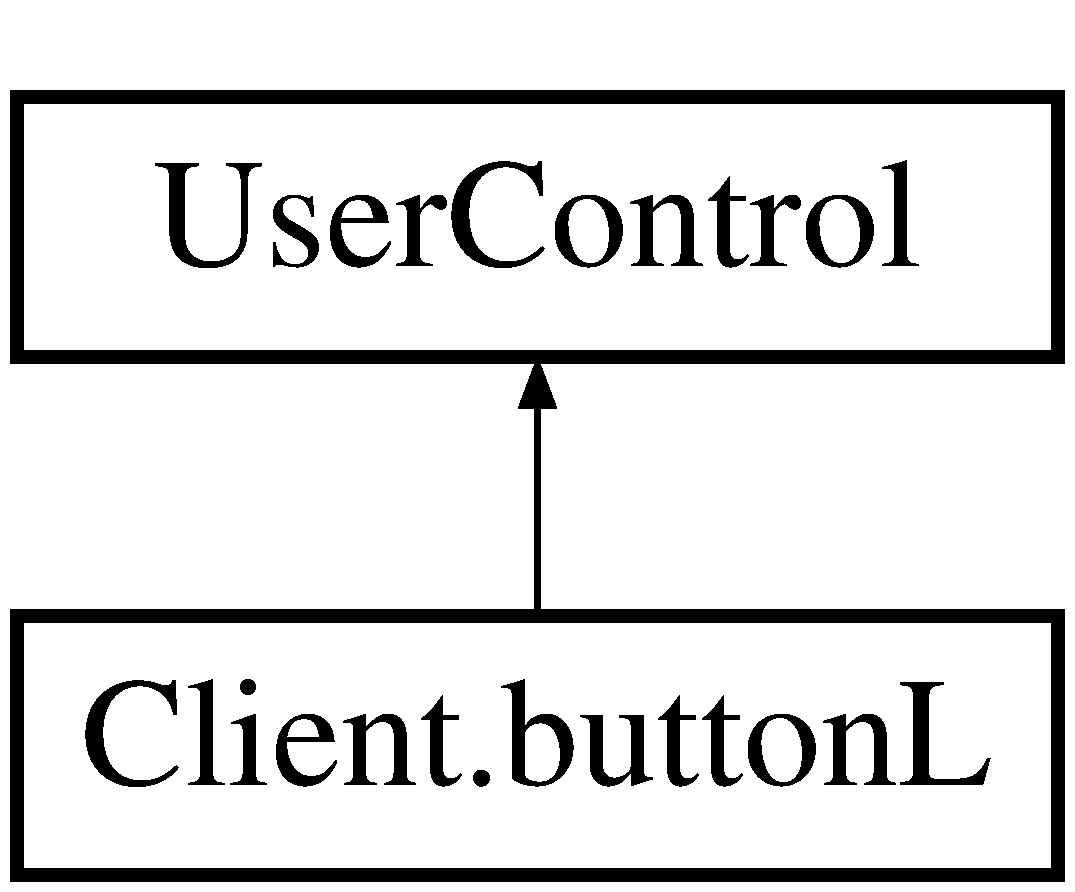
\includegraphics[height=2.000000cm]{class_client_1_1button_l}
\end{center}
\end{figure}
\subsection*{Protected Member Functions}
\begin{DoxyCompactItemize}
\item 
override void \hyperlink{class_client_1_1button_l_ac6fa538126a25fce97996f189914812a}{Dispose} (bool disposing)
\begin{DoxyCompactList}\small\item\em Освободить все используемые ресурсы. \end{DoxyCompactList}\end{DoxyCompactItemize}


\subsection{Member Function Documentation}
\hypertarget{class_client_1_1button_l_ac6fa538126a25fce97996f189914812a}{}\label{class_client_1_1button_l_ac6fa538126a25fce97996f189914812a} 
\index{Client\+::buttonL@{Client\+::buttonL}!Dispose@{Dispose}}
\index{Dispose@{Dispose}!Client\+::buttonL@{Client\+::buttonL}}
\subsubsection{\texorpdfstring{Dispose()}{Dispose()}}
{\footnotesize\ttfamily override void Client.\+button\+L.\+Dispose (\begin{DoxyParamCaption}\item[{bool}]{disposing }\end{DoxyParamCaption})\hspace{0.3cm}{\ttfamily [inline]}, {\ttfamily [protected]}}



Освободить все используемые ресурсы. 


\begin{DoxyParams}{Parameters}
{\em disposing} & истинно, если управляемый ресурс должен быть удален; иначе ложно.\\
\hline
\end{DoxyParams}


The documentation for this class was generated from the following files\+:\begin{DoxyCompactItemize}
\item 
C\+:/\+Users/саша/\+Documents/\+Visual Studio 2015/\+Projects/\+Forex2.\+0/\+Client/button\+L.\+cs\item 
C\+:/\+Users/саша/\+Documents/\+Visual Studio 2015/\+Projects/\+Forex2.\+0/\+Client/button\+L.\+Designer.\+cs\end{DoxyCompactItemize}

\hypertarget{class_client_1_1_chart_q}{}\section{Client.\+ChartQ Class Reference}
\label{class_client_1_1_chart_q}\index{Client.\+ChartQ@{Client.\+ChartQ}}


Класс для изменения чарта и задание линий  


\subsection*{Public Member Functions}
\begin{DoxyCompactItemize}
\item 
Series \hyperlink{class_client_1_1_chart_q_a23b497a1946f947333d86f5987f2321b}{ext\+Series} (string Chart\+Area, Chart\+Value\+Type X\+Value\+Type, Series\+Chart\+Type Line, int Border\+Width)
\begin{DoxyCompactList}\small\item\em Метод задания параметров линии \end{DoxyCompactList}\item 
Chart \hyperlink{class_client_1_1_chart_q_ae25afd3337c1460af47d6e26b69ba2df}{Quote} (Chart graphic, string value)
\begin{DoxyCompactList}\small\item\em Метод задания параметров линии \end{DoxyCompactList}\end{DoxyCompactItemize}


\subsection{Detailed Description}
Класс для изменения чарта и задание линий 



\subsection{Member Function Documentation}
\hypertarget{class_client_1_1_chart_q_a23b497a1946f947333d86f5987f2321b}{}\label{class_client_1_1_chart_q_a23b497a1946f947333d86f5987f2321b} 
\index{Client\+::\+ChartQ@{Client\+::\+ChartQ}!ext\+Series@{ext\+Series}}
\index{ext\+Series@{ext\+Series}!Client\+::\+ChartQ@{Client\+::\+ChartQ}}
\subsubsection{\texorpdfstring{ext\+Series()}{extSeries()}}
{\footnotesize\ttfamily Series Client.\+Chart\+Q.\+ext\+Series (\begin{DoxyParamCaption}\item[{string}]{Chart\+Area,  }\item[{Chart\+Value\+Type}]{X\+Value\+Type,  }\item[{Series\+Chart\+Type}]{Line,  }\item[{int}]{Border\+Width }\end{DoxyParamCaption})\hspace{0.3cm}{\ttfamily [inline]}}



Метод задания параметров линии 


\begin{DoxyParams}{Parameters}
{\em Chart\+Area} & Название чарта к которому привязана линия\\
\hline
{\em X\+Value\+Type} & Тип чарта\\
\hline
{\em Line} & тип линии\\
\hline
{\em Border\+Width} & толщина линии\\
\hline
\end{DoxyParams}
\hypertarget{class_client_1_1_chart_q_ae25afd3337c1460af47d6e26b69ba2df}{}\label{class_client_1_1_chart_q_ae25afd3337c1460af47d6e26b69ba2df} 
\index{Client\+::\+ChartQ@{Client\+::\+ChartQ}!Quote@{Quote}}
\index{Quote@{Quote}!Client\+::\+ChartQ@{Client\+::\+ChartQ}}
\subsubsection{\texorpdfstring{Quote()}{Quote()}}
{\footnotesize\ttfamily Chart Client.\+Chart\+Q.\+Quote (\begin{DoxyParamCaption}\item[{Chart}]{graphic,  }\item[{string}]{value }\end{DoxyParamCaption})\hspace{0.3cm}{\ttfamily [inline]}}



Метод задания параметров линии 



The documentation for this class was generated from the following file\+:\begin{DoxyCompactItemize}
\item 
C\+:/\+Users/саша/\+Documents/\+Visual Studio 2015/\+Projects/\+Forex2.\+0/\+Client/Chat\+Q.\+cs\end{DoxyCompactItemize}

\hypertarget{class_client_1_1_class_s_m_a}{}\section{Client.\+Class\+S\+MA Class Reference}
\label{class_client_1_1_class_s_m_a}\index{Client.\+Class\+S\+MA@{Client.\+Class\+S\+MA}}


Вычисление линии S\+MA +  


\subsection*{Public Member Functions}
\begin{DoxyCompactItemize}
\item 
\hypertarget{class_client_1_1_class_s_m_a_a5834fc0ea86725568c9a153da1a78238}{}\label{class_client_1_1_class_s_m_a_a5834fc0ea86725568c9a153da1a78238} 
void {\bfseries Add} (int Sglag, List$<$ double $>$ point)
\item 
List$<$ double $>$ \hyperlink{class_client_1_1_class_s_m_a_a9155b88e63c8eacb884e05c9bfa64799}{Get\+Sred} ()
\begin{DoxyCompactList}\small\item\em Выдача точек S\+MA + \end{DoxyCompactList}\end{DoxyCompactItemize}


\subsection{Detailed Description}
Вычисление линии S\+MA + 



\subsection{Member Function Documentation}
\hypertarget{class_client_1_1_class_s_m_a_a9155b88e63c8eacb884e05c9bfa64799}{}\label{class_client_1_1_class_s_m_a_a9155b88e63c8eacb884e05c9bfa64799} 
\index{Client\+::\+Class\+S\+MA@{Client\+::\+Class\+S\+MA}!Get\+Sred@{Get\+Sred}}
\index{Get\+Sred@{Get\+Sred}!Client\+::\+Class\+S\+MA@{Client\+::\+Class\+S\+MA}}
\subsubsection{\texorpdfstring{Get\+Sred()}{GetSred()}}
{\footnotesize\ttfamily List$<$double$>$ Client.\+Class\+S\+M\+A.\+Get\+Sred (\begin{DoxyParamCaption}{ }\end{DoxyParamCaption})\hspace{0.3cm}{\ttfamily [inline]}}



Выдача точек S\+MA + 



The documentation for this class was generated from the following file\+:\begin{DoxyCompactItemize}
\item 
C\+:/\+Users/саша/\+Documents/\+Visual Studio 2015/\+Projects/\+Forex2.\+0/\+Client/S\+M\+A.\+cs\end{DoxyCompactItemize}

\hypertarget{class_client_1_1_close_deal}{}\section{Client.\+Close\+Deal Class Reference}
\label{class_client_1_1_close_deal}\index{Client.\+Close\+Deal@{Client.\+Close\+Deal}}


Класс по закрытию сделки  


Inheritance diagram for Client.\+Close\+Deal\+:\begin{figure}[H]
\begin{center}
\leavevmode
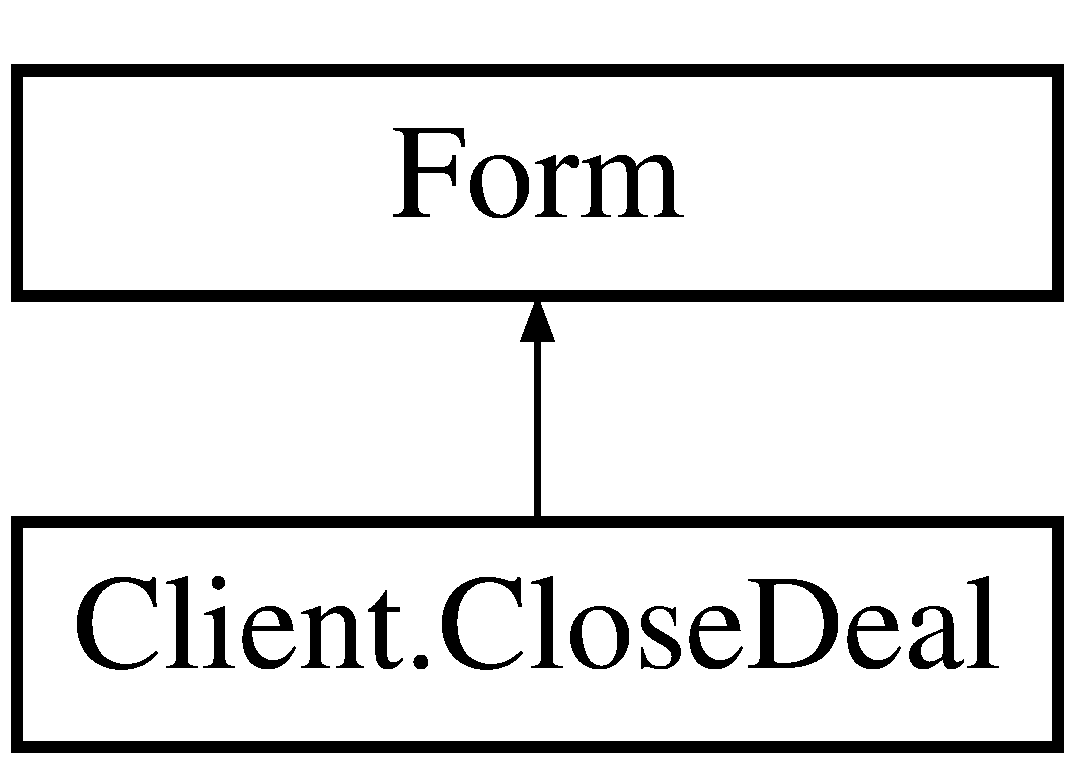
\includegraphics[height=2.000000cm]{class_client_1_1_close_deal}
\end{center}
\end{figure}
\subsection*{Public Member Functions}
\begin{DoxyCompactItemize}
\item 
\hyperlink{class_client_1_1_close_deal_a405298882ae55f600ca25b00898159f3}{Close\+Deal} ()
\begin{DoxyCompactList}\small\item\em Инициализация компонентов \end{DoxyCompactList}\item 
void \hyperlink{class_client_1_1_close_deal_a2693cd775d06cfc1a31b68523eac5b86}{Close\+Deal\+\_\+\+Load} (object sender, Event\+Args e)
\begin{DoxyCompactList}\small\item\em Закрытие сделки 
\begin{DoxyParams}{Parameters}
{\em sender} & Объект события\\
\hline
{\em e} & ТСобытие\\
\hline
\end{DoxyParams}
\end{DoxyCompactList}\item 
void \hyperlink{class_client_1_1_close_deal_a540ae3b166b32a9957fc86d27f39dbd1}{List\+Form} (string Rus, string Eng, List$<$ \hyperlink{class_client_1_1_deal}{Deal} $>$ S\+E\+LL)
\begin{DoxyCompactList}\small\item\em Добавление сделок в лист формы 
\begin{DoxyParams}{Parameters}
{\em Rus} & русский язык\\
\hline
{\em Eng} & английский\\
\hline
{\em S\+E\+LL} & Продажа\\
\hline
\end{DoxyParams}
\end{DoxyCompactList}\item 
\hypertarget{class_client_1_1_close_deal_a1a032066cdeea7795714a3dea0271805}{}\label{class_client_1_1_close_deal_a1a032066cdeea7795714a3dea0271805} 
double {\bfseries Profit} (double chislo, double profit, string Value)
\item 
void \hyperlink{class_client_1_1_close_deal_a99ff7b19b66fefbcc3ea5b45bf02a88d}{Close} (double chislo, double profit, string Value, Date\+Time Date, List$<$ double $>$ iter\+Data, int d\+Time)
\begin{DoxyCompactList}\small\item\em Выбор и закрытие ордера 
\begin{DoxyParams}{Parameters}
{\em chislo} & Значение выбранной сделки\\
\hline
{\em profit} & Прибыль\\
\hline
{\em Value} & Значение + операция над ней\\
\hline
{\em Date} & Время сделки\\
\hline
{\em iter\+Data} & Контейнер\\
\hline
{\em d\+Time} & Время в формате Unix\+Time\\
\hline
\end{DoxyParams}
\end{DoxyCompactList}\end{DoxyCompactItemize}
\subsection*{Public Attributes}
\begin{DoxyCompactItemize}
\item 
\hypertarget{class_client_1_1_close_deal_ad68485ab502db5b884eff7a204a32c1b}{}\label{class_client_1_1_close_deal_ad68485ab502db5b884eff7a204a32c1b} 
double {\bfseries Spred}
\end{DoxyCompactItemize}
\subsection*{Protected Member Functions}
\begin{DoxyCompactItemize}
\item 
override void \hyperlink{class_client_1_1_close_deal_ac72c1f7f73882a1af7d84ec19ad56bc8}{Dispose} (bool disposing)
\begin{DoxyCompactList}\small\item\em Clean up any resources being used. \end{DoxyCompactList}\end{DoxyCompactItemize}


\subsection{Detailed Description}
Класс по закрытию сделки 



\subsection{Constructor \& Destructor Documentation}
\hypertarget{class_client_1_1_close_deal_a405298882ae55f600ca25b00898159f3}{}\label{class_client_1_1_close_deal_a405298882ae55f600ca25b00898159f3} 
\index{Client\+::\+Close\+Deal@{Client\+::\+Close\+Deal}!Close\+Deal@{Close\+Deal}}
\index{Close\+Deal@{Close\+Deal}!Client\+::\+Close\+Deal@{Client\+::\+Close\+Deal}}
\subsubsection{\texorpdfstring{Close\+Deal()}{CloseDeal()}}
{\footnotesize\ttfamily Client.\+Close\+Deal.\+Close\+Deal (\begin{DoxyParamCaption}{ }\end{DoxyParamCaption})\hspace{0.3cm}{\ttfamily [inline]}}



Инициализация компонентов 



\subsection{Member Function Documentation}
\hypertarget{class_client_1_1_close_deal_a99ff7b19b66fefbcc3ea5b45bf02a88d}{}\label{class_client_1_1_close_deal_a99ff7b19b66fefbcc3ea5b45bf02a88d} 
\index{Client\+::\+Close\+Deal@{Client\+::\+Close\+Deal}!Close@{Close}}
\index{Close@{Close}!Client\+::\+Close\+Deal@{Client\+::\+Close\+Deal}}
\subsubsection{\texorpdfstring{Close()}{Close()}}
{\footnotesize\ttfamily void Client.\+Close\+Deal.\+Close (\begin{DoxyParamCaption}\item[{double}]{chislo,  }\item[{double}]{profit,  }\item[{string}]{Value,  }\item[{Date\+Time}]{Date,  }\item[{List$<$ double $>$}]{iter\+Data,  }\item[{int}]{d\+Time }\end{DoxyParamCaption})\hspace{0.3cm}{\ttfamily [inline]}}



Выбор и закрытие ордера 
\begin{DoxyParams}{Parameters}
{\em chislo} & Значение выбранной сделки\\
\hline
{\em profit} & Прибыль\\
\hline
{\em Value} & Значение + операция над ней\\
\hline
{\em Date} & Время сделки\\
\hline
{\em iter\+Data} & Контейнер\\
\hline
{\em d\+Time} & Время в формате Unix\+Time\\
\hline
\end{DoxyParams}


\hypertarget{class_client_1_1_close_deal_a2693cd775d06cfc1a31b68523eac5b86}{}\label{class_client_1_1_close_deal_a2693cd775d06cfc1a31b68523eac5b86} 
\index{Client\+::\+Close\+Deal@{Client\+::\+Close\+Deal}!Close\+Deal\+\_\+\+Load@{Close\+Deal\+\_\+\+Load}}
\index{Close\+Deal\+\_\+\+Load@{Close\+Deal\+\_\+\+Load}!Client\+::\+Close\+Deal@{Client\+::\+Close\+Deal}}
\subsubsection{\texorpdfstring{Close\+Deal\+\_\+\+Load()}{CloseDeal\_Load()}}
{\footnotesize\ttfamily void Client.\+Close\+Deal.\+Close\+Deal\+\_\+\+Load (\begin{DoxyParamCaption}\item[{object}]{sender,  }\item[{Event\+Args}]{e }\end{DoxyParamCaption})\hspace{0.3cm}{\ttfamily [inline]}}



Закрытие сделки 
\begin{DoxyParams}{Parameters}
{\em sender} & Объект события\\
\hline
{\em e} & ТСобытие\\
\hline
\end{DoxyParams}


\hypertarget{class_client_1_1_close_deal_ac72c1f7f73882a1af7d84ec19ad56bc8}{}\label{class_client_1_1_close_deal_ac72c1f7f73882a1af7d84ec19ad56bc8} 
\index{Client\+::\+Close\+Deal@{Client\+::\+Close\+Deal}!Dispose@{Dispose}}
\index{Dispose@{Dispose}!Client\+::\+Close\+Deal@{Client\+::\+Close\+Deal}}
\subsubsection{\texorpdfstring{Dispose()}{Dispose()}}
{\footnotesize\ttfamily override void Client.\+Close\+Deal.\+Dispose (\begin{DoxyParamCaption}\item[{bool}]{disposing }\end{DoxyParamCaption})\hspace{0.3cm}{\ttfamily [inline]}, {\ttfamily [protected]}}



Clean up any resources being used. 


\begin{DoxyParams}{Parameters}
{\em disposing} & true if managed resources should be disposed; otherwise, false.\\
\hline
\end{DoxyParams}
\hypertarget{class_client_1_1_close_deal_a540ae3b166b32a9957fc86d27f39dbd1}{}\label{class_client_1_1_close_deal_a540ae3b166b32a9957fc86d27f39dbd1} 
\index{Client\+::\+Close\+Deal@{Client\+::\+Close\+Deal}!List\+Form@{List\+Form}}
\index{List\+Form@{List\+Form}!Client\+::\+Close\+Deal@{Client\+::\+Close\+Deal}}
\subsubsection{\texorpdfstring{List\+Form()}{ListForm()}}
{\footnotesize\ttfamily void Client.\+Close\+Deal.\+List\+Form (\begin{DoxyParamCaption}\item[{string}]{Rus,  }\item[{string}]{Eng,  }\item[{List$<$ \hyperlink{class_client_1_1_deal}{Deal} $>$}]{S\+E\+LL }\end{DoxyParamCaption})\hspace{0.3cm}{\ttfamily [inline]}}



Добавление сделок в лист формы 
\begin{DoxyParams}{Parameters}
{\em Rus} & русский язык\\
\hline
{\em Eng} & английский\\
\hline
{\em S\+E\+LL} & Продажа\\
\hline
\end{DoxyParams}




The documentation for this class was generated from the following files\+:\begin{DoxyCompactItemize}
\item 
C\+:/\+Users/саша/\+Documents/\+Visual Studio 2015/\+Projects/\+Forex2.\+0/\+Client/Close\+Deal.\+cs\item 
C\+:/\+Users/саша/\+Documents/\+Visual Studio 2015/\+Projects/\+Forex2.\+0/\+Client/Close\+Deal.\+Designer.\+cs\end{DoxyCompactItemize}

\hypertarget{class_client_1_1_deal}{}\section{Client.\+Deal Class Reference}
\label{class_client_1_1_deal}\index{Client.\+Deal@{Client.\+Deal}}


Класс сохраняющий сделки  


\subsection*{Public Member Functions}
\begin{DoxyCompactItemize}
\item 
\hyperlink{class_client_1_1_deal_ac0c16b651799c774f86eaaf1cbe608b2}{Deal} (bool type\+Deal, List$<$ double $>$ Array\+Inet\+Quotes, int tic)
\begin{DoxyCompactList}\small\item\em Constructor deal + \end{DoxyCompactList}\item 
void \hyperlink{class_client_1_1_deal_a18be29256aca8a79b8da771d9c139ecb}{Trade} ()
\begin{DoxyCompactList}\small\item\em Метод запоминание совершенных покупок и продаж \end{DoxyCompactList}\item 
double \hyperlink{class_client_1_1_deal_a6719991014f189438bffe5e5d01f1767}{Value} ()
\begin{DoxyCompactList}\small\item\em Мето возвращение значения \end{DoxyCompactList}\end{DoxyCompactItemize}


\subsection{Detailed Description}
Класс сохраняющий сделки 



\subsection{Constructor \& Destructor Documentation}
\hypertarget{class_client_1_1_deal_ac0c16b651799c774f86eaaf1cbe608b2}{}\label{class_client_1_1_deal_ac0c16b651799c774f86eaaf1cbe608b2} 
\index{Client\+::\+Deal@{Client\+::\+Deal}!Deal@{Deal}}
\index{Deal@{Deal}!Client\+::\+Deal@{Client\+::\+Deal}}
\subsubsection{\texorpdfstring{Deal()}{Deal()}}
{\footnotesize\ttfamily Client.\+Deal.\+Deal (\begin{DoxyParamCaption}\item[{bool}]{type\+Deal,  }\item[{List$<$ double $>$}]{Array\+Inet\+Quotes,  }\item[{int}]{tic }\end{DoxyParamCaption})\hspace{0.3cm}{\ttfamily [inline]}}



Constructor deal + 


\begin{DoxyParams}{Parameters}
{\em type\+Deal} & Тип сделки true покупка false продажа\\
\hline
{\em Array\+Inet\+Quotes} & Массив котировок после подключения\\
\hline
{\em tic} & текущее время от начала торгов\\
\hline
\end{DoxyParams}


\subsection{Member Function Documentation}
\hypertarget{class_client_1_1_deal_a18be29256aca8a79b8da771d9c139ecb}{}\label{class_client_1_1_deal_a18be29256aca8a79b8da771d9c139ecb} 
\index{Client\+::\+Deal@{Client\+::\+Deal}!Trade@{Trade}}
\index{Trade@{Trade}!Client\+::\+Deal@{Client\+::\+Deal}}
\subsubsection{\texorpdfstring{Trade()}{Trade()}}
{\footnotesize\ttfamily void Client.\+Deal.\+Trade (\begin{DoxyParamCaption}{ }\end{DoxyParamCaption})\hspace{0.3cm}{\ttfamily [inline]}}



Метод запоминание совершенных покупок и продаж 


\begin{DoxyParams}{Parameters}
{\em buy} & \\
\hline
{\em bufferS} & Массив покупки\\
\hline
{\em tic} & текущее время отначала торгов\\
\hline
\end{DoxyParams}
\hypertarget{class_client_1_1_deal_a6719991014f189438bffe5e5d01f1767}{}\label{class_client_1_1_deal_a6719991014f189438bffe5e5d01f1767} 
\index{Client\+::\+Deal@{Client\+::\+Deal}!Value@{Value}}
\index{Value@{Value}!Client\+::\+Deal@{Client\+::\+Deal}}
\subsubsection{\texorpdfstring{Value()}{Value()}}
{\footnotesize\ttfamily double Client.\+Deal.\+Value (\begin{DoxyParamCaption}{ }\end{DoxyParamCaption})\hspace{0.3cm}{\ttfamily [inline]}}



Мето возвращение значения 



The documentation for this class was generated from the following file\+:\begin{DoxyCompactItemize}
\item 
C\+:/\+Users/саша/\+Documents/\+Visual Studio 2015/\+Projects/\+Forex2.\+0/\+Client/deal.\+cs\end{DoxyCompactItemize}

\hypertarget{class_client_1_1_directory_work}{}\section{Client.\+Directory\+Work Class Reference}
\label{class_client_1_1_directory_work}\index{Client.\+Directory\+Work@{Client.\+Directory\+Work}}


Класс для работы с директорией  


\subsection*{Static Public Member Functions}
\begin{DoxyCompactItemize}
\item 
static void \hyperlink{class_client_1_1_directory_work_a42fbcc188b41ea61bdb1cc67397b2c69}{Set} (string path\+Directory)
\begin{DoxyCompactList}\small\item\em Проверка существования директории с уведомлением \end{DoxyCompactList}\end{DoxyCompactItemize}


\subsection{Detailed Description}
Класс для работы с директорией 



\subsection{Member Function Documentation}
\hypertarget{class_client_1_1_directory_work_a42fbcc188b41ea61bdb1cc67397b2c69}{}\label{class_client_1_1_directory_work_a42fbcc188b41ea61bdb1cc67397b2c69} 
\index{Client\+::\+Directory\+Work@{Client\+::\+Directory\+Work}!Set@{Set}}
\index{Set@{Set}!Client\+::\+Directory\+Work@{Client\+::\+Directory\+Work}}
\subsubsection{\texorpdfstring{Set()}{Set()}}
{\footnotesize\ttfamily static void Client.\+Directory\+Work.\+Set (\begin{DoxyParamCaption}\item[{string}]{path\+Directory }\end{DoxyParamCaption})\hspace{0.3cm}{\ttfamily [inline]}, {\ttfamily [static]}}



Проверка существования директории с уведомлением 


\begin{DoxyParams}{Parameters}
{\em path\+Directory} & путь к директории\\
\hline
\end{DoxyParams}


The documentation for this class was generated from the following file\+:\begin{DoxyCompactItemize}
\item 
C\+:/\+Users/саша/\+Documents/\+Visual Studio 2015/\+Projects/\+Forex2.\+0/\+Client/Directory\+Insspection.\+cs\end{DoxyCompactItemize}

\hypertarget{class_client_1_1_display}{}\section{Client.\+Display Class Reference}
\label{class_client_1_1_display}\index{Client.\+Display@{Client.\+Display}}


Класс для адаптации размеров окон под размеры экрана  


\subsection*{Static Public Member Functions}
\begin{DoxyCompactItemize}
\item 
static Point \hyperlink{class_client_1_1_display_a205e226e42ca66974f905c8d3c4a0d1c}{customized\+Point} (int xc, int yc)
\begin{DoxyCompactList}\small\item\em Преобразование окон под различные экраны компьютера \end{DoxyCompactList}\end{DoxyCompactItemize}


\subsection{Detailed Description}
Класс для адаптации размеров окон под размеры экрана 



\subsection{Member Function Documentation}
\hypertarget{class_client_1_1_display_a205e226e42ca66974f905c8d3c4a0d1c}{}\label{class_client_1_1_display_a205e226e42ca66974f905c8d3c4a0d1c} 
\index{Client\+::\+Display@{Client\+::\+Display}!customized\+Point@{customized\+Point}}
\index{customized\+Point@{customized\+Point}!Client\+::\+Display@{Client\+::\+Display}}
\subsubsection{\texorpdfstring{customized\+Point()}{customizedPoint()}}
{\footnotesize\ttfamily static Point Client.\+Display.\+customized\+Point (\begin{DoxyParamCaption}\item[{int}]{xc,  }\item[{int}]{yc }\end{DoxyParamCaption})\hspace{0.3cm}{\ttfamily [inline]}, {\ttfamily [static]}}



Преобразование окон под различные экраны компьютера 


\begin{DoxyParams}{Parameters}
{\em xc} & координат по x\\
\hline
{\em yc} & координаты по y\\
\hline
\end{DoxyParams}


The documentation for this class was generated from the following file\+:\begin{DoxyCompactItemize}
\item 
C\+:/\+Users/саша/\+Documents/\+Visual Studio 2015/\+Projects/\+Forex2.\+0/\+Client/Display.\+cs\end{DoxyCompactItemize}

\hypertarget{class_client_1_1_event}{}\section{Client.\+Event Class Reference}
\label{class_client_1_1_event}\index{Client.\+Event@{Client.\+Event}}


Событие  




\subsection{Detailed Description}
Событие 



The documentation for this class was generated from the following file\+:\begin{DoxyCompactItemize}
\item 
C\+:/\+Users/саша/\+Documents/\+Visual Studio 2015/\+Projects/\+Forex2.\+0/\+Client/Event.\+cs\end{DoxyCompactItemize}

\hypertarget{class_client_1_1_exel}{}\section{Client.\+Exel Class Reference}
\label{class_client_1_1_exel}\index{Client.\+Exel@{Client.\+Exel}}


Класс отвечающий за работу с \hyperlink{class_client_1_1_exel}{Exel}  


\subsection*{Public Member Functions}
\begin{DoxyCompactItemize}
\item 
\hypertarget{class_client_1_1_exel_a6b7582eff5018df59b27dcff7665bed5}{}\label{class_client_1_1_exel_a6b7582eff5018df59b27dcff7665bed5} 
void {\bfseries E\+Save} (Data\+Grid\+View data\+Grid\+View1)
\item 
\hypertarget{class_client_1_1_exel_aad4f1e39cc59aaf42bf4bd78799f4619}{}\label{class_client_1_1_exel_aad4f1e39cc59aaf42bf4bd78799f4619} 
void {\bfseries E\+Load} (Data\+Grid\+View data\+Grid\+View1)
\item 
\hypertarget{class_client_1_1_exel_accd3e811c70509ef58988c273575b8b4}{}\label{class_client_1_1_exel_accd3e811c70509ef58988c273575b8b4} 
List$<$ List$<$ string $>$ $>$ {\bfseries E\+Save\+Up} (Data\+Grid\+View data\+Grid\+View1)
\end{DoxyCompactItemize}


\subsection{Detailed Description}
Класс отвечающий за работу с \hyperlink{class_client_1_1_exel}{Exel} 



The documentation for this class was generated from the following file\+:\begin{DoxyCompactItemize}
\item 
C\+:/\+Users/саша/\+Documents/\+Visual Studio 2015/\+Projects/\+Forex2.\+0/\+Client/Exel.\+cs\end{DoxyCompactItemize}

\hypertarget{class_client_1_1_extend_button}{}\section{Client.\+Extend\+Button Class Reference}
\label{class_client_1_1_extend_button}\index{Client.\+Extend\+Button@{Client.\+Extend\+Button}}


Класс расширяюший базовые возможности кнопки  


Inheritance diagram for Client.\+Extend\+Button\+:\begin{figure}[H]
\begin{center}
\leavevmode
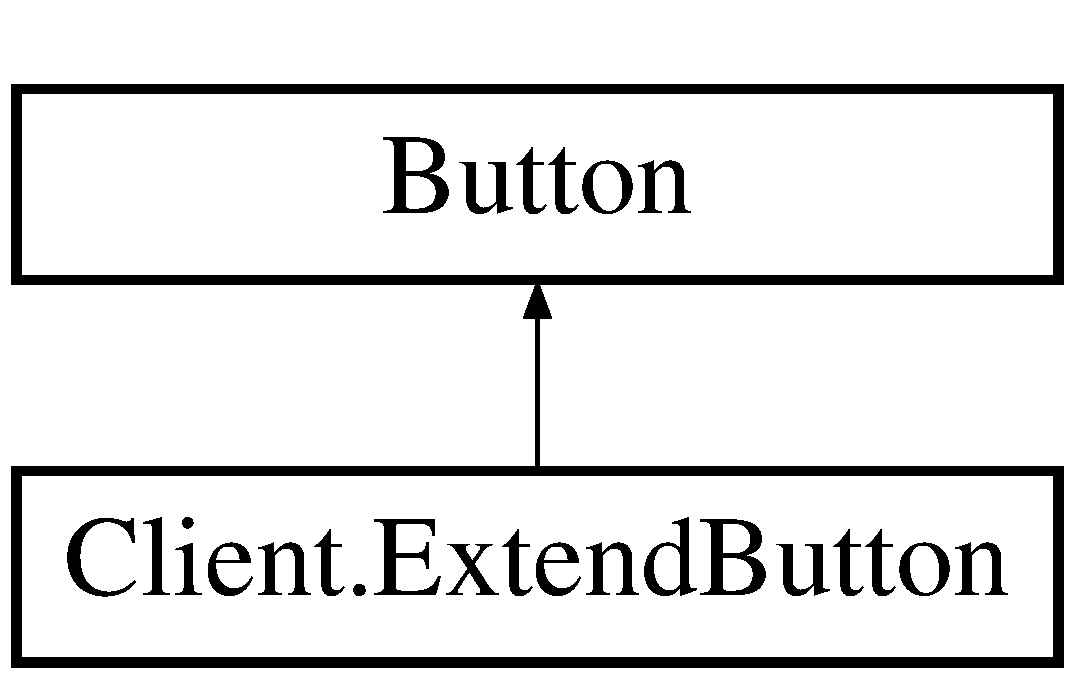
\includegraphics[height=2.000000cm]{class_client_1_1_extend_button}
\end{center}
\end{figure}
\subsection*{Public Member Functions}
\begin{DoxyCompactItemize}
\item 
\hypertarget{class_client_1_1_extend_button_aab2bbc128bf0463f40c1572372711ed4}{}\label{class_client_1_1_extend_button_aab2bbc128bf0463f40c1572372711ed4} 
void {\bfseries Translate} (string name1)
\end{DoxyCompactItemize}
\subsection*{Public Attributes}
\begin{DoxyCompactItemize}
\item 
string \hyperlink{class_client_1_1_extend_button_a980571f04f44336a1fb9f662a79f760f}{rus\+Lan}
\begin{DoxyCompactList}\small\item\em Наименование на русском \end{DoxyCompactList}\item 
string \hyperlink{class_client_1_1_extend_button_aaa4299e5b2843a9fddaced18352c44a4}{eng\+Lan}
\begin{DoxyCompactList}\small\item\em Наименование на английском \end{DoxyCompactList}\end{DoxyCompactItemize}


\subsection{Detailed Description}
Класс расширяюший базовые возможности кнопки 



\subsection{Member Data Documentation}
\hypertarget{class_client_1_1_extend_button_aaa4299e5b2843a9fddaced18352c44a4}{}\label{class_client_1_1_extend_button_aaa4299e5b2843a9fddaced18352c44a4} 
\index{Client\+::\+Extend\+Button@{Client\+::\+Extend\+Button}!eng\+Lan@{eng\+Lan}}
\index{eng\+Lan@{eng\+Lan}!Client\+::\+Extend\+Button@{Client\+::\+Extend\+Button}}
\subsubsection{\texorpdfstring{eng\+Lan}{engLan}}
{\footnotesize\ttfamily string Client.\+Extend\+Button.\+eng\+Lan}



Наименование на английском 

\hypertarget{class_client_1_1_extend_button_a980571f04f44336a1fb9f662a79f760f}{}\label{class_client_1_1_extend_button_a980571f04f44336a1fb9f662a79f760f} 
\index{Client\+::\+Extend\+Button@{Client\+::\+Extend\+Button}!rus\+Lan@{rus\+Lan}}
\index{rus\+Lan@{rus\+Lan}!Client\+::\+Extend\+Button@{Client\+::\+Extend\+Button}}
\subsubsection{\texorpdfstring{rus\+Lan}{rusLan}}
{\footnotesize\ttfamily string Client.\+Extend\+Button.\+rus\+Lan}



Наименование на русском 



The documentation for this class was generated from the following file\+:\begin{DoxyCompactItemize}
\item 
C\+:/\+Users/саша/\+Documents/\+Visual Studio 2015/\+Projects/\+Forex2.\+0/\+Client/Extend\+Button.\+cs\end{DoxyCompactItemize}

\hypertarget{class_client_1_1_extend_checkbox}{}\section{Client.\+Extend\+Checkbox Class Reference}
\label{class_client_1_1_extend_checkbox}\index{Client.\+Extend\+Checkbox@{Client.\+Extend\+Checkbox}}


Класс расширяюший базовые возможности чекбокс  


Inheritance diagram for Client.\+Extend\+Checkbox\+:\begin{figure}[H]
\begin{center}
\leavevmode
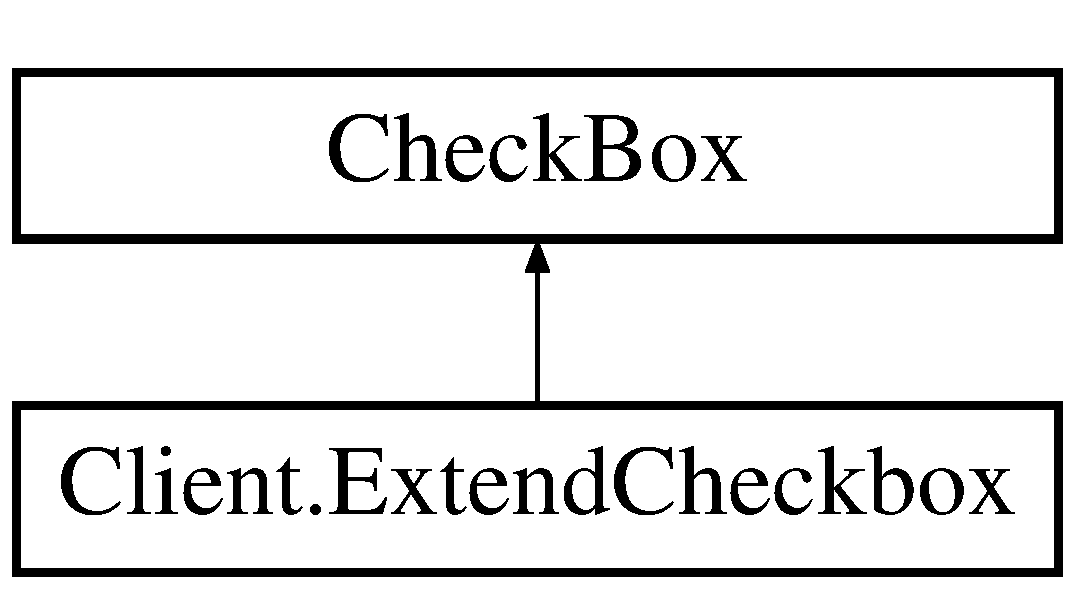
\includegraphics[height=2.000000cm]{class_client_1_1_extend_checkbox}
\end{center}
\end{figure}
\subsection*{Public Member Functions}
\begin{DoxyCompactItemize}
\item 
\hypertarget{class_client_1_1_extend_checkbox_af93d9c763cced54baaed7741f3003e57}{}\label{class_client_1_1_extend_checkbox_af93d9c763cced54baaed7741f3003e57} 
void {\bfseries Translate} (string name1)
\end{DoxyCompactItemize}
\subsection*{Public Attributes}
\begin{DoxyCompactItemize}
\item 
string \hyperlink{class_client_1_1_extend_checkbox_a89930618ff403ae6714aaf3b6983bf81}{rus\+Lan}
\begin{DoxyCompactList}\small\item\em Наименование на русском \end{DoxyCompactList}\item 
string \hyperlink{class_client_1_1_extend_checkbox_ae2b4e37f89f3ead5c2f873d014f62cb7}{eng\+Lan}
\begin{DoxyCompactList}\small\item\em Наименование на английском \end{DoxyCompactList}\end{DoxyCompactItemize}


\subsection{Detailed Description}
Класс расширяюший базовые возможности чекбокс 



\subsection{Member Data Documentation}
\hypertarget{class_client_1_1_extend_checkbox_ae2b4e37f89f3ead5c2f873d014f62cb7}{}\label{class_client_1_1_extend_checkbox_ae2b4e37f89f3ead5c2f873d014f62cb7} 
\index{Client\+::\+Extend\+Checkbox@{Client\+::\+Extend\+Checkbox}!eng\+Lan@{eng\+Lan}}
\index{eng\+Lan@{eng\+Lan}!Client\+::\+Extend\+Checkbox@{Client\+::\+Extend\+Checkbox}}
\subsubsection{\texorpdfstring{eng\+Lan}{engLan}}
{\footnotesize\ttfamily string Client.\+Extend\+Checkbox.\+eng\+Lan}



Наименование на английском 

\hypertarget{class_client_1_1_extend_checkbox_a89930618ff403ae6714aaf3b6983bf81}{}\label{class_client_1_1_extend_checkbox_a89930618ff403ae6714aaf3b6983bf81} 
\index{Client\+::\+Extend\+Checkbox@{Client\+::\+Extend\+Checkbox}!rus\+Lan@{rus\+Lan}}
\index{rus\+Lan@{rus\+Lan}!Client\+::\+Extend\+Checkbox@{Client\+::\+Extend\+Checkbox}}
\subsubsection{\texorpdfstring{rus\+Lan}{rusLan}}
{\footnotesize\ttfamily string Client.\+Extend\+Checkbox.\+rus\+Lan}



Наименование на русском 



The documentation for this class was generated from the following file\+:\begin{DoxyCompactItemize}
\item 
C\+:/\+Users/саша/\+Documents/\+Visual Studio 2015/\+Projects/\+Forex2.\+0/\+Client/Extend\+Checkbox.\+cs\end{DoxyCompactItemize}

\hypertarget{class_client_1_1_extend_label}{}\section{Client.\+Extend\+Label Class Reference}
\label{class_client_1_1_extend_label}\index{Client.\+Extend\+Label@{Client.\+Extend\+Label}}


Класс расширяюший базовые возможности лабел  


Inheritance diagram for Client.\+Extend\+Label\+:\begin{figure}[H]
\begin{center}
\leavevmode
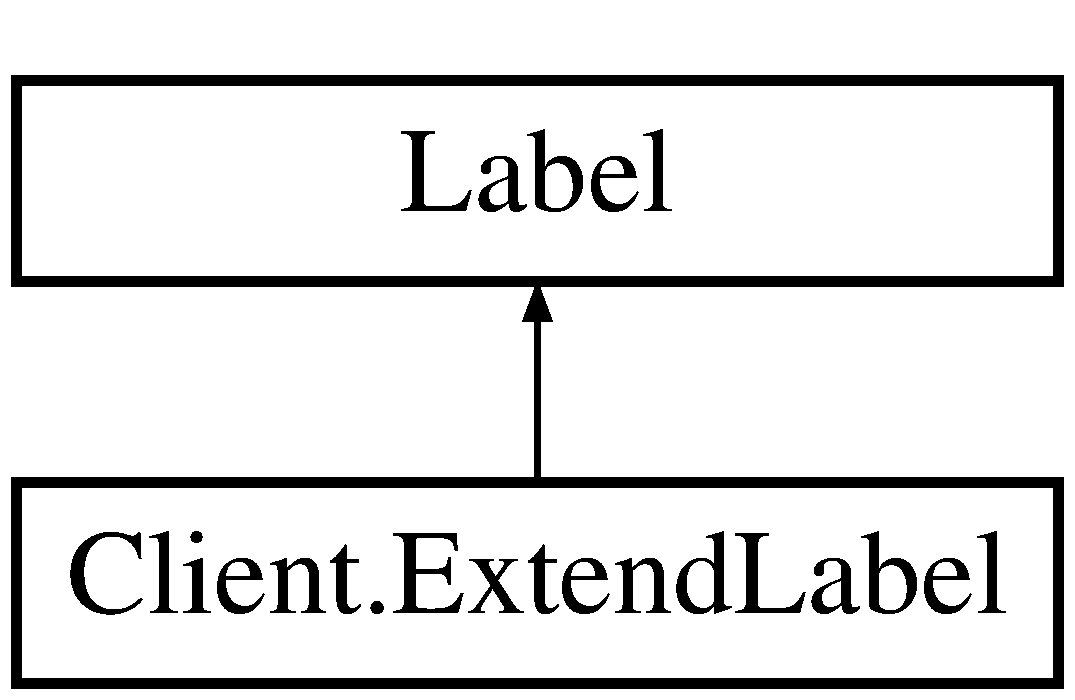
\includegraphics[height=2.000000cm]{class_client_1_1_extend_label}
\end{center}
\end{figure}
\subsection*{Public Member Functions}
\begin{DoxyCompactItemize}
\item 
\hypertarget{class_client_1_1_extend_label_abdbb5351d8f1e8e5a0a3901dfc67044b}{}\label{class_client_1_1_extend_label_abdbb5351d8f1e8e5a0a3901dfc67044b} 
void {\bfseries Translate} (string name1)
\end{DoxyCompactItemize}
\subsection*{Public Attributes}
\begin{DoxyCompactItemize}
\item 
string \hyperlink{class_client_1_1_extend_label_a77d9ce34371d09953d0fd6423abbc6c6}{rus\+Lan}
\begin{DoxyCompactList}\small\item\em Наименование на русском \end{DoxyCompactList}\item 
string \hyperlink{class_client_1_1_extend_label_a75adae5701c1a1a81f6dca5928d171c2}{eng\+Lan}
\begin{DoxyCompactList}\small\item\em Наименование на английском \end{DoxyCompactList}\end{DoxyCompactItemize}


\subsection{Detailed Description}
Класс расширяюший базовые возможности лабел 



\subsection{Member Data Documentation}
\hypertarget{class_client_1_1_extend_label_a75adae5701c1a1a81f6dca5928d171c2}{}\label{class_client_1_1_extend_label_a75adae5701c1a1a81f6dca5928d171c2} 
\index{Client\+::\+Extend\+Label@{Client\+::\+Extend\+Label}!eng\+Lan@{eng\+Lan}}
\index{eng\+Lan@{eng\+Lan}!Client\+::\+Extend\+Label@{Client\+::\+Extend\+Label}}
\subsubsection{\texorpdfstring{eng\+Lan}{engLan}}
{\footnotesize\ttfamily string Client.\+Extend\+Label.\+eng\+Lan}



Наименование на английском 

\hypertarget{class_client_1_1_extend_label_a77d9ce34371d09953d0fd6423abbc6c6}{}\label{class_client_1_1_extend_label_a77d9ce34371d09953d0fd6423abbc6c6} 
\index{Client\+::\+Extend\+Label@{Client\+::\+Extend\+Label}!rus\+Lan@{rus\+Lan}}
\index{rus\+Lan@{rus\+Lan}!Client\+::\+Extend\+Label@{Client\+::\+Extend\+Label}}
\subsubsection{\texorpdfstring{rus\+Lan}{rusLan}}
{\footnotesize\ttfamily string Client.\+Extend\+Label.\+rus\+Lan}



Наименование на русском 



The documentation for this class was generated from the following file\+:\begin{DoxyCompactItemize}
\item 
C\+:/\+Users/саша/\+Documents/\+Visual Studio 2015/\+Projects/\+Forex2.\+0/\+Client/Extend\+Label.\+cs\end{DoxyCompactItemize}

\hypertarget{class_client_1_1_extend_tool_strip_menu_item}{}\section{Client.\+Extend\+Tool\+Strip\+Menu\+Item Class Reference}
\label{class_client_1_1_extend_tool_strip_menu_item}\index{Client.\+Extend\+Tool\+Strip\+Menu\+Item@{Client.\+Extend\+Tool\+Strip\+Menu\+Item}}


Класс расширяюший базовые возможности меню  


Inheritance diagram for Client.\+Extend\+Tool\+Strip\+Menu\+Item\+:\begin{figure}[H]
\begin{center}
\leavevmode
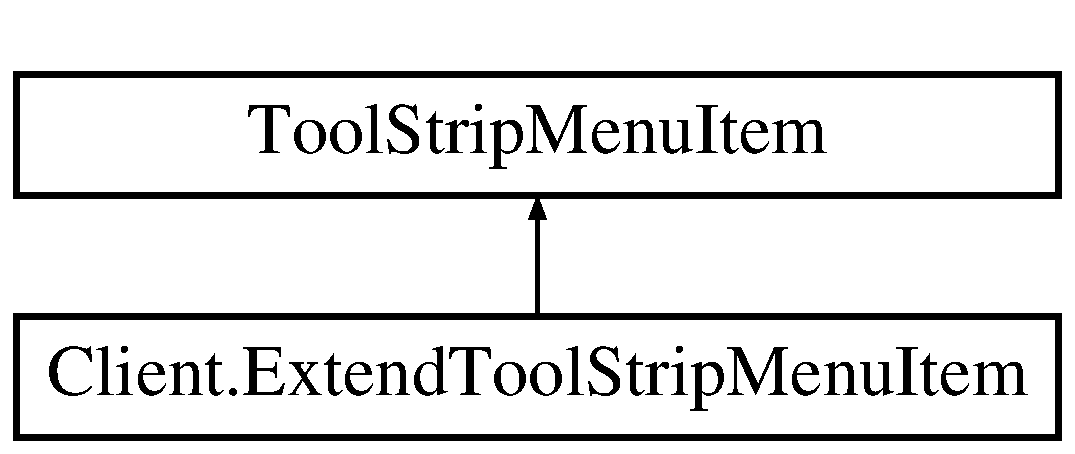
\includegraphics[height=2.000000cm]{class_client_1_1_extend_tool_strip_menu_item}
\end{center}
\end{figure}
\subsection*{Public Member Functions}
\begin{DoxyCompactItemize}
\item 
\hypertarget{class_client_1_1_extend_tool_strip_menu_item_a148e298d46585db26cc44a47ad50292f}{}\label{class_client_1_1_extend_tool_strip_menu_item_a148e298d46585db26cc44a47ad50292f} 
void {\bfseries Translate} (string name1)
\end{DoxyCompactItemize}
\subsection*{Public Attributes}
\begin{DoxyCompactItemize}
\item 
string \hyperlink{class_client_1_1_extend_tool_strip_menu_item_abae1637b49f6f25f2a08eaa0a1e60fdc}{rus\+Lan}
\begin{DoxyCompactList}\small\item\em Наименование на русском \end{DoxyCompactList}\item 
string \hyperlink{class_client_1_1_extend_tool_strip_menu_item_a71d1d698ca4315da70a0c2553c017c5f}{eng\+Lan}
\begin{DoxyCompactList}\small\item\em Наименование на английском \end{DoxyCompactList}\end{DoxyCompactItemize}


\subsection{Detailed Description}
Класс расширяюший базовые возможности меню 



\subsection{Member Data Documentation}
\hypertarget{class_client_1_1_extend_tool_strip_menu_item_a71d1d698ca4315da70a0c2553c017c5f}{}\label{class_client_1_1_extend_tool_strip_menu_item_a71d1d698ca4315da70a0c2553c017c5f} 
\index{Client\+::\+Extend\+Tool\+Strip\+Menu\+Item@{Client\+::\+Extend\+Tool\+Strip\+Menu\+Item}!eng\+Lan@{eng\+Lan}}
\index{eng\+Lan@{eng\+Lan}!Client\+::\+Extend\+Tool\+Strip\+Menu\+Item@{Client\+::\+Extend\+Tool\+Strip\+Menu\+Item}}
\subsubsection{\texorpdfstring{eng\+Lan}{engLan}}
{\footnotesize\ttfamily string Client.\+Extend\+Tool\+Strip\+Menu\+Item.\+eng\+Lan}



Наименование на английском 

\hypertarget{class_client_1_1_extend_tool_strip_menu_item_abae1637b49f6f25f2a08eaa0a1e60fdc}{}\label{class_client_1_1_extend_tool_strip_menu_item_abae1637b49f6f25f2a08eaa0a1e60fdc} 
\index{Client\+::\+Extend\+Tool\+Strip\+Menu\+Item@{Client\+::\+Extend\+Tool\+Strip\+Menu\+Item}!rus\+Lan@{rus\+Lan}}
\index{rus\+Lan@{rus\+Lan}!Client\+::\+Extend\+Tool\+Strip\+Menu\+Item@{Client\+::\+Extend\+Tool\+Strip\+Menu\+Item}}
\subsubsection{\texorpdfstring{rus\+Lan}{rusLan}}
{\footnotesize\ttfamily string Client.\+Extend\+Tool\+Strip\+Menu\+Item.\+rus\+Lan}



Наименование на русском 



The documentation for this class was generated from the following file\+:\begin{DoxyCompactItemize}
\item 
C\+:/\+Users/саша/\+Documents/\+Visual Studio 2015/\+Projects/\+Forex2.\+0/\+Client/Extend\+Tool\+Strip\+Menu\+Item.\+cs\end{DoxyCompactItemize}

\hypertarget{class_client_1_1_file_inspection}{}\section{Client.\+File\+Inspection Class Reference}
\label{class_client_1_1_file_inspection}\index{Client.\+File\+Inspection@{Client.\+File\+Inspection}}


Классд для проверки существования файла  


Inheritance diagram for Client.\+File\+Inspection\+:\begin{figure}[H]
\begin{center}
\leavevmode
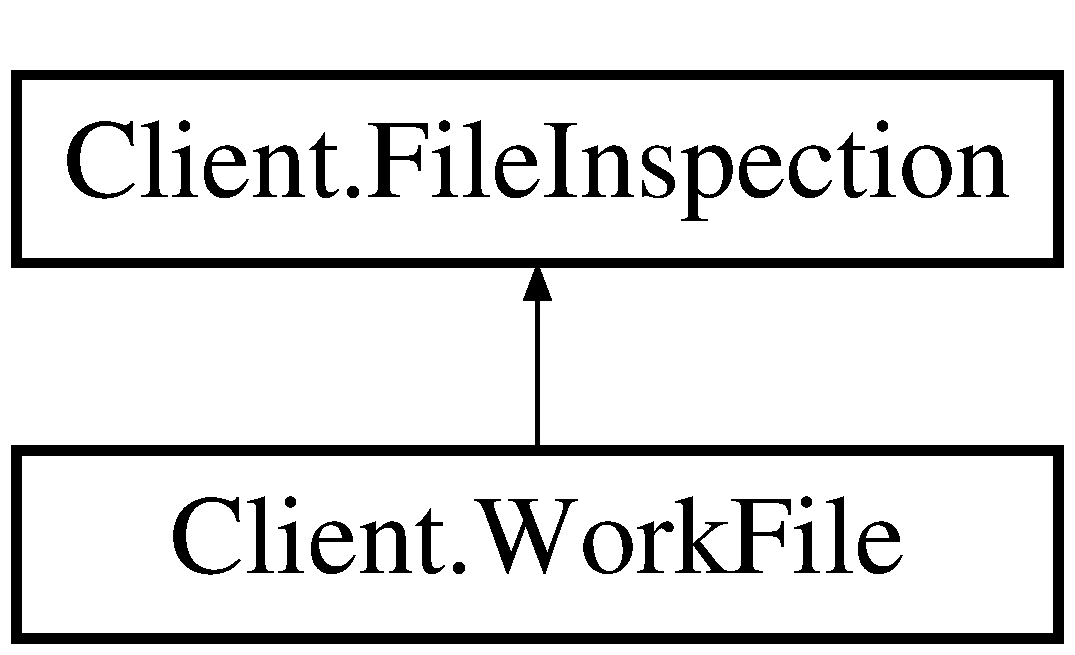
\includegraphics[height=2.000000cm]{class_client_1_1_file_inspection}
\end{center}
\end{figure}
\subsection*{Static Public Member Functions}
\begin{DoxyCompactItemize}
\item 
static void \hyperlink{class_client_1_1_file_inspection_a10b45d302a1a339e008f14b66f071889}{Set} (string path\+File)
\begin{DoxyCompactList}\small\item\em Приветствие нового пользователя \end{DoxyCompactList}\end{DoxyCompactItemize}


\subsection{Detailed Description}
Классд для проверки существования файла 



\subsection{Member Function Documentation}
\hypertarget{class_client_1_1_file_inspection_a10b45d302a1a339e008f14b66f071889}{}\label{class_client_1_1_file_inspection_a10b45d302a1a339e008f14b66f071889} 
\index{Client\+::\+File\+Inspection@{Client\+::\+File\+Inspection}!Set@{Set}}
\index{Set@{Set}!Client\+::\+File\+Inspection@{Client\+::\+File\+Inspection}}
\subsubsection{\texorpdfstring{Set()}{Set()}}
{\footnotesize\ttfamily static void Client.\+File\+Inspection.\+Set (\begin{DoxyParamCaption}\item[{string}]{path\+File }\end{DoxyParamCaption})\hspace{0.3cm}{\ttfamily [inline]}, {\ttfamily [static]}}



Приветствие нового пользователя 


\begin{DoxyParams}{Parameters}
{\em path\+File} & Путь к файлу \\
\hline
\end{DoxyParams}


The documentation for this class was generated from the following file\+:\begin{DoxyCompactItemize}
\item 
C\+:/\+Users/саша/\+Documents/\+Visual Studio 2015/\+Projects/\+Forex2.\+0/\+Client/File\+Inspection.\+cs\end{DoxyCompactItemize}

\hypertarget{class_client_1_1_graph_y}{}\section{Client.\+GraphY Class Reference}
\label{class_client_1_1_graph_y}\index{Client.\+GraphY@{Client.\+GraphY}}


класс отвечающий за диапазон графика  


\subsection*{Public Member Functions}
\begin{DoxyCompactItemize}
\item 
void \hyperlink{class_client_1_1_graph_y_ad6d507d05b33972eeeda5c3fe8f4354a}{scopeY} (Chart chart1, double Nowcurency)
\begin{DoxyCompactList}\small\item\em Метод отвечающий за диапазон графика \end{DoxyCompactList}\end{DoxyCompactItemize}


\subsection{Detailed Description}
класс отвечающий за диапазон графика 



\subsection{Member Function Documentation}
\hypertarget{class_client_1_1_graph_y_ad6d507d05b33972eeeda5c3fe8f4354a}{}\label{class_client_1_1_graph_y_ad6d507d05b33972eeeda5c3fe8f4354a} 
\index{Client\+::\+GraphY@{Client\+::\+GraphY}!scopeY@{scopeY}}
\index{scopeY@{scopeY}!Client\+::\+GraphY@{Client\+::\+GraphY}}
\subsubsection{\texorpdfstring{scope\+Y()}{scopeY()}}
{\footnotesize\ttfamily void Client.\+Graph\+Y.\+scopeY (\begin{DoxyParamCaption}\item[{Chart}]{chart1,  }\item[{double}]{Nowcurency }\end{DoxyParamCaption})\hspace{0.3cm}{\ttfamily [inline]}}



Метод отвечающий за диапазон графика 


\begin{DoxyParams}{Parameters}
{\em char1} & График\\
\hline
{\em Nowcurency} & текущее значение котировки\\
\hline
\end{DoxyParams}


The documentation for this class was generated from the following file\+:\begin{DoxyCompactItemize}
\item 
C\+:/\+Users/саша/\+Documents/\+Visual Studio 2015/\+Projects/\+Forex2.\+0/\+Client/Graph\+Y.\+cs\end{DoxyCompactItemize}

\hypertarget{class_client_1_1_help}{}\section{Client.\+Help Class Reference}
\label{class_client_1_1_help}\index{Client.\+Help@{Client.\+Help}}


Класс отвечающий за окно \hyperlink{class_client_1_1_help}{Help}  


Inheritance diagram for Client.\+Help\+:\begin{figure}[H]
\begin{center}
\leavevmode
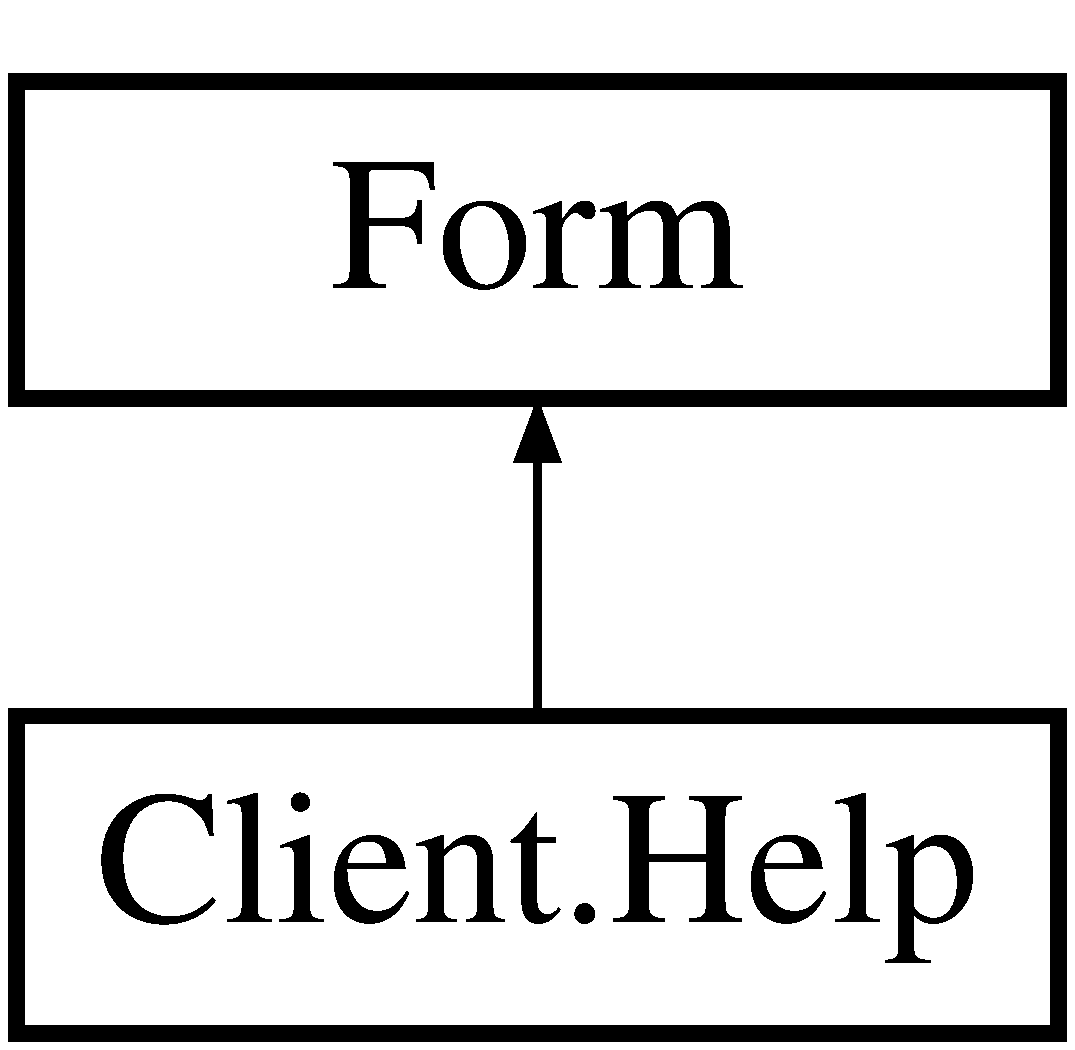
\includegraphics[height=2.000000cm]{class_client_1_1_help}
\end{center}
\end{figure}
\subsection*{Protected Member Functions}
\begin{DoxyCompactItemize}
\item 
override void \hyperlink{class_client_1_1_help_a9cab13fd059101ccbbd6e25e0157fe27}{Dispose} (bool disposing)
\begin{DoxyCompactList}\small\item\em Clean up any resources being used. \end{DoxyCompactList}\end{DoxyCompactItemize}


\subsection{Detailed Description}
Класс отвечающий за окно \hyperlink{class_client_1_1_help}{Help} 



\subsection{Member Function Documentation}
\hypertarget{class_client_1_1_help_a9cab13fd059101ccbbd6e25e0157fe27}{}\label{class_client_1_1_help_a9cab13fd059101ccbbd6e25e0157fe27} 
\index{Client\+::\+Help@{Client\+::\+Help}!Dispose@{Dispose}}
\index{Dispose@{Dispose}!Client\+::\+Help@{Client\+::\+Help}}
\subsubsection{\texorpdfstring{Dispose()}{Dispose()}}
{\footnotesize\ttfamily override void Client.\+Help.\+Dispose (\begin{DoxyParamCaption}\item[{bool}]{disposing }\end{DoxyParamCaption})\hspace{0.3cm}{\ttfamily [inline]}, {\ttfamily [protected]}}



Clean up any resources being used. 


\begin{DoxyParams}{Parameters}
{\em disposing} & true if managed resources should be disposed; otherwise, false.\\
\hline
\end{DoxyParams}


The documentation for this class was generated from the following files\+:\begin{DoxyCompactItemize}
\item 
C\+:/\+Users/саша/\+Documents/\+Visual Studio 2015/\+Projects/\+Forex2.\+0/\+Client/Help.\+cs\item 
C\+:/\+Users/саша/\+Documents/\+Visual Studio 2015/\+Projects/\+Forex2.\+0/\+Client/Help.\+Designer.\+cs\end{DoxyCompactItemize}

\hypertarget{interface_client_1_1_interface}{}\section{Client.\+Interface Interface Reference}
\label{interface_client_1_1_interface}\index{Client.\+Interface@{Client.\+Interface}}


Интерфейс  


\subsection*{Public Member Functions}
\begin{DoxyCompactItemize}
\item 
\hypertarget{interface_client_1_1_interface_ad1c4a8a9032601195bfcbd3fbae45cb2}{}\label{interface_client_1_1_interface_ad1c4a8a9032601195bfcbd3fbae45cb2} 
void {\bfseries get\+Data} ()
\item 
\hypertarget{interface_client_1_1_interface_a20f90fb1316acffc0184159261657dc7}{}\label{interface_client_1_1_interface_a20f90fb1316acffc0184159261657dc7} 
void {\bfseries set\+Data} ()
\end{DoxyCompactItemize}


\subsection{Detailed Description}
Интерфейс 



The documentation for this interface was generated from the following file\+:\begin{DoxyCompactItemize}
\item 
C\+:/\+Users/саша/\+Documents/\+Visual Studio 2015/\+Projects/\+Forex2.\+0/\+Client/Interface.\+cs\end{DoxyCompactItemize}

\hypertarget{class_client_1_1_internet}{}\section{Client.\+Internet Class Reference}
\label{class_client_1_1_internet}\index{Client.\+Internet@{Client.\+Internet}}


Класс отечающий за работу с интернетом  


Inheritance diagram for Client.\+Internet\+:\begin{figure}[H]
\begin{center}
\leavevmode
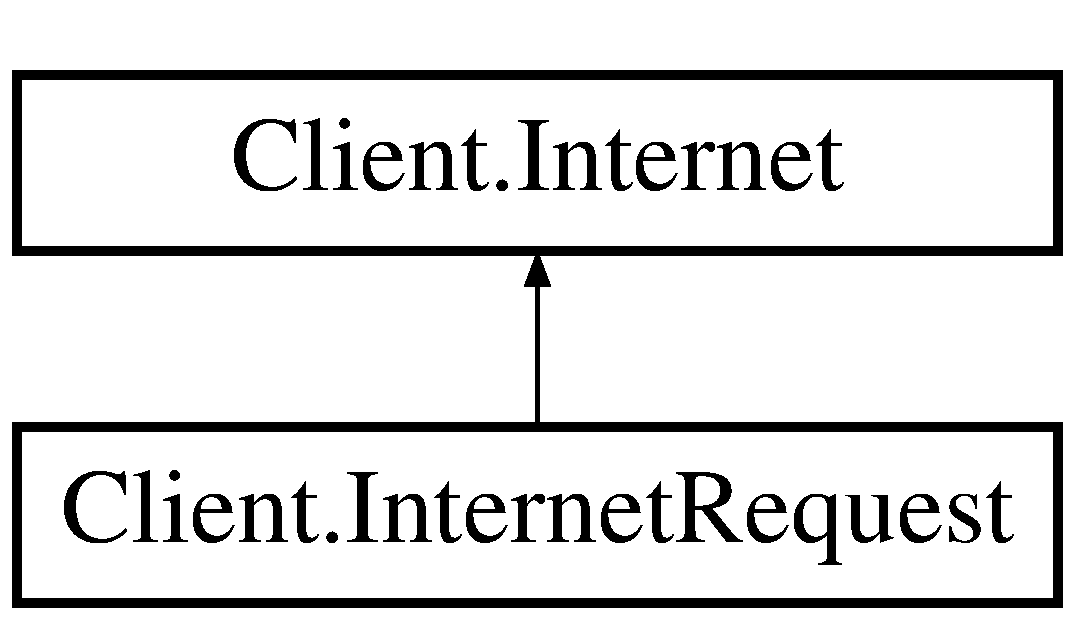
\includegraphics[height=2.000000cm]{class_client_1_1_internet}
\end{center}
\end{figure}
\subsection*{Public Member Functions}
\begin{DoxyCompactItemize}
\item 
bool \hyperlink{class_client_1_1_internet_a9dd75df149ccd3f37a7808371734df6e}{Try\+Con} (string value, object sync, bool internet\+Action\+Finished)
\begin{DoxyCompactList}\small\item\em Этот метод проверяет интернет соединение и переводит программу в автономный режим в случае его отсутсвия + \end{DoxyCompactList}\item 
bool \hyperlink{class_client_1_1_internet_ac5dffd376bcb63c31d30e676c42ea16b}{Reqest\+Inet} (string value, bool internet\+Action\+Finished)
\begin{DoxyCompactList}\small\item\em Этот метод проверяет интернет соединение и переводит программу в автономный режим в случае его отсутсвия + \end{DoxyCompactList}\item 
string \hyperlink{class_client_1_1_internet_acb1ebd5d0e24109a5bf17ffc40d3b4d9}{First\+Connect\+BD} (string value, string path\+File, int number, string patch)
\begin{DoxyCompactList}\small\item\em Этот метод находит из базы данных последнее время котировки и делает запрос на сайт и сохраняет в БД \end{DoxyCompactList}\item 
void \hyperlink{class_client_1_1_internet_a7264aa476ec385c1cb78e21e6c011f18}{First\+Connect} (string value, string path\+File)
\begin{DoxyCompactList}\small\item\em Этот метод находит из файла последнее время котировки и делает запрос на сайт сохраняя в тот же файл \end{DoxyCompactList}\item 
string \hyperlink{class_client_1_1_internet_afeff19924124e7ca32b7509d4b055610}{Connect\+I\+BD} (int posl\+Time, int limit, string value)
\item 
void \hyperlink{class_client_1_1_internet_a1cd19828884f2508d44f8af4a2975ace}{ConnectI} (int posl\+Time, int limit, string path\+File, string value)
\begin{DoxyCompactList}\small\item\em Этот метод получает последнее время сохраненное в файле, путь и валюту для запроса на сервер за данными и их сохранение в локальный файл \end{DoxyCompactList}\item 
Stream\+Reader \hyperlink{class_client_1_1_internet_a670f0e1e3b71b1c88f6895adf7eefe97}{Conection} (int limit, double poslT, string value)
\begin{DoxyCompactList}\small\item\em Метод отвечающий за запрос за данными + \end{DoxyCompactList}\item 
string \hyperlink{class_client_1_1_internet_a17349606c7aad5494e14ec2f216b6b3b}{Task\+Connect} (string value)
\begin{DoxyCompactList}\small\item\em Метод загрузки данных + \end{DoxyCompactList}\end{DoxyCompactItemize}


\subsection{Detailed Description}
Класс отечающий за работу с интернетом 



\subsection{Member Function Documentation}
\hypertarget{class_client_1_1_internet_a670f0e1e3b71b1c88f6895adf7eefe97}{}\label{class_client_1_1_internet_a670f0e1e3b71b1c88f6895adf7eefe97} 
\index{Client\+::\+Internet@{Client\+::\+Internet}!Conection@{Conection}}
\index{Conection@{Conection}!Client\+::\+Internet@{Client\+::\+Internet}}
\subsubsection{\texorpdfstring{Conection()}{Conection()}}
{\footnotesize\ttfamily Stream\+Reader Client.\+Internet.\+Conection (\begin{DoxyParamCaption}\item[{int}]{limit,  }\item[{double}]{poslT,  }\item[{string}]{value }\end{DoxyParamCaption})\hspace{0.3cm}{\ttfamily [inline]}}



Метод отвечающий за запрос за данными + 


\begin{DoxyParams}{Parameters}
{\em limit} & Предел кол-\/ва записей с сервера\\
\hline
{\em value} & Выбранная котировка\\
\hline
{\em poslT} & Последнее время\\
\hline
\end{DoxyParams}
\begin{DoxyReturn}{Returns}
Возвращает полученные записи из интернета
\end{DoxyReturn}
\hypertarget{class_client_1_1_internet_a1cd19828884f2508d44f8af4a2975ace}{}\label{class_client_1_1_internet_a1cd19828884f2508d44f8af4a2975ace} 
\index{Client\+::\+Internet@{Client\+::\+Internet}!ConnectI@{ConnectI}}
\index{ConnectI@{ConnectI}!Client\+::\+Internet@{Client\+::\+Internet}}
\subsubsection{\texorpdfstring{Connect\+I()}{ConnectI()}}
{\footnotesize\ttfamily void Client.\+Internet.\+ConnectI (\begin{DoxyParamCaption}\item[{int}]{posl\+Time,  }\item[{int}]{limit,  }\item[{string}]{path\+File,  }\item[{string}]{value }\end{DoxyParamCaption})\hspace{0.3cm}{\ttfamily [inline]}}



Этот метод получает последнее время сохраненное в файле, путь и валюту для запроса на сервер за данными и их сохранение в локальный файл 


\begin{DoxyParams}{Parameters}
{\em posl\+Time} & Последнее сохранившиеся время\\
\hline
{\em limit} & Предел кол-\/ва записей с сервера\\
\hline
{\em path\+File} & Путь к файлу\\
\hline
{\em value} & Выбранная котировка\\
\hline
\end{DoxyParams}
\hypertarget{class_client_1_1_internet_afeff19924124e7ca32b7509d4b055610}{}\label{class_client_1_1_internet_afeff19924124e7ca32b7509d4b055610} 
\index{Client\+::\+Internet@{Client\+::\+Internet}!Connect\+I\+BD@{Connect\+I\+BD}}
\index{Connect\+I\+BD@{Connect\+I\+BD}!Client\+::\+Internet@{Client\+::\+Internet}}
\subsubsection{\texorpdfstring{Connect\+I\+B\+D()}{ConnectIBD()}}
{\footnotesize\ttfamily string Client.\+Internet.\+Connect\+I\+BD (\begin{DoxyParamCaption}\item[{int}]{posl\+Time,  }\item[{int}]{limit,  }\item[{string}]{value }\end{DoxyParamCaption})\hspace{0.3cm}{\ttfamily [inline]}}





Этот метод получает последнее время сохраненное в файле, путь и валюту для запроса на сервер за данными и их сохранение в локальный файл 


\begin{DoxyParams}{Parameters}
{\em posl\+Time} & Последнее сохранившиеся время\\
\hline
{\em limit} & Предел кол-\/ва записей с сервера\\
\hline
{\em value} & Выбранная котировка\\
\hline
\end{DoxyParams}
\hypertarget{class_client_1_1_internet_a7264aa476ec385c1cb78e21e6c011f18}{}\label{class_client_1_1_internet_a7264aa476ec385c1cb78e21e6c011f18} 
\index{Client\+::\+Internet@{Client\+::\+Internet}!First\+Connect@{First\+Connect}}
\index{First\+Connect@{First\+Connect}!Client\+::\+Internet@{Client\+::\+Internet}}
\subsubsection{\texorpdfstring{First\+Connect()}{FirstConnect()}}
{\footnotesize\ttfamily void Client.\+Internet.\+First\+Connect (\begin{DoxyParamCaption}\item[{string}]{value,  }\item[{string}]{path\+File }\end{DoxyParamCaption})\hspace{0.3cm}{\ttfamily [inline]}}



Этот метод находит из файла последнее время котировки и делает запрос на сайт сохраняя в тот же файл 


\begin{DoxyParams}{Parameters}
{\em path\+File} & Путь к файлу\\
\hline
{\em value} & Выбранная котировка\\
\hline
\end{DoxyParams}
\hypertarget{class_client_1_1_internet_acb1ebd5d0e24109a5bf17ffc40d3b4d9}{}\label{class_client_1_1_internet_acb1ebd5d0e24109a5bf17ffc40d3b4d9} 
\index{Client\+::\+Internet@{Client\+::\+Internet}!First\+Connect\+BD@{First\+Connect\+BD}}
\index{First\+Connect\+BD@{First\+Connect\+BD}!Client\+::\+Internet@{Client\+::\+Internet}}
\subsubsection{\texorpdfstring{First\+Connect\+B\+D()}{FirstConnectBD()}}
{\footnotesize\ttfamily string Client.\+Internet.\+First\+Connect\+BD (\begin{DoxyParamCaption}\item[{string}]{value,  }\item[{string}]{path\+File,  }\item[{int}]{number,  }\item[{string}]{patch }\end{DoxyParamCaption})\hspace{0.3cm}{\ttfamily [inline]}}



Этот метод находит из базы данных последнее время котировки и делает запрос на сайт и сохраняет в БД 


\begin{DoxyParams}{Parameters}
{\em path\+File} & Путь к файлу\\
\hline
{\em value} & Выбранная котировка\\
\hline
{\em number} & кол-\/во чисел\\
\hline
\end{DoxyParams}
\hypertarget{class_client_1_1_internet_ac5dffd376bcb63c31d30e676c42ea16b}{}\label{class_client_1_1_internet_ac5dffd376bcb63c31d30e676c42ea16b} 
\index{Client\+::\+Internet@{Client\+::\+Internet}!Reqest\+Inet@{Reqest\+Inet}}
\index{Reqest\+Inet@{Reqest\+Inet}!Client\+::\+Internet@{Client\+::\+Internet}}
\subsubsection{\texorpdfstring{Reqest\+Inet()}{ReqestInet()}}
{\footnotesize\ttfamily bool Client.\+Internet.\+Reqest\+Inet (\begin{DoxyParamCaption}\item[{string}]{value,  }\item[{bool}]{internet\+Action\+Finished }\end{DoxyParamCaption})\hspace{0.3cm}{\ttfamily [inline]}}



Этот метод проверяет интернет соединение и переводит программу в автономный режим в случае его отсутсвия + 


\begin{DoxyParams}{Parameters}
{\em value} & Название котировки\\
\hline
{\em internet\+Action\+Finished} & оповещении о Окончание запроса \\
\hline
\end{DoxyParams}
\hypertarget{class_client_1_1_internet_a17349606c7aad5494e14ec2f216b6b3b}{}\label{class_client_1_1_internet_a17349606c7aad5494e14ec2f216b6b3b} 
\index{Client\+::\+Internet@{Client\+::\+Internet}!Task\+Connect@{Task\+Connect}}
\index{Task\+Connect@{Task\+Connect}!Client\+::\+Internet@{Client\+::\+Internet}}
\subsubsection{\texorpdfstring{Task\+Connect()}{TaskConnect()}}
{\footnotesize\ttfamily string Client.\+Internet.\+Task\+Connect (\begin{DoxyParamCaption}\item[{string}]{value }\end{DoxyParamCaption})\hspace{0.3cm}{\ttfamily [inline]}}



Метод загрузки данных + 


\begin{DoxyParams}{Parameters}
{\em value} & Котировка\\
\hline
\end{DoxyParams}
\hypertarget{class_client_1_1_internet_a9dd75df149ccd3f37a7808371734df6e}{}\label{class_client_1_1_internet_a9dd75df149ccd3f37a7808371734df6e} 
\index{Client\+::\+Internet@{Client\+::\+Internet}!Try\+Con@{Try\+Con}}
\index{Try\+Con@{Try\+Con}!Client\+::\+Internet@{Client\+::\+Internet}}
\subsubsection{\texorpdfstring{Try\+Con()}{TryCon()}}
{\footnotesize\ttfamily bool Client.\+Internet.\+Try\+Con (\begin{DoxyParamCaption}\item[{string}]{value,  }\item[{object}]{sync,  }\item[{bool}]{internet\+Action\+Finished }\end{DoxyParamCaption})\hspace{0.3cm}{\ttfamily [inline]}}



Этот метод проверяет интернет соединение и переводит программу в автономный режим в случае его отсутсвия + 


\begin{DoxyParams}{Parameters}
{\em value} & Название котировки\\
\hline
{\em object} & \\
\hline
{\em internet\+Action\+Finished} & оповещении о Окончание запроса \\
\hline
\end{DoxyParams}


The documentation for this class was generated from the following file\+:\begin{DoxyCompactItemize}
\item 
C\+:/\+Users/саша/\+Documents/\+Visual Studio 2015/\+Projects/\+Forex2.\+0/\+Client/Internet.\+cs\end{DoxyCompactItemize}

\hypertarget{class_client_1_1_internet_request}{}\section{Client.\+Internet\+Request Class Reference}
\label{class_client_1_1_internet_request}\index{Client.\+Internet\+Request@{Client.\+Internet\+Request}}


Класс интернет запрос  


Inheritance diagram for Client.\+Internet\+Request\+:\begin{figure}[H]
\begin{center}
\leavevmode
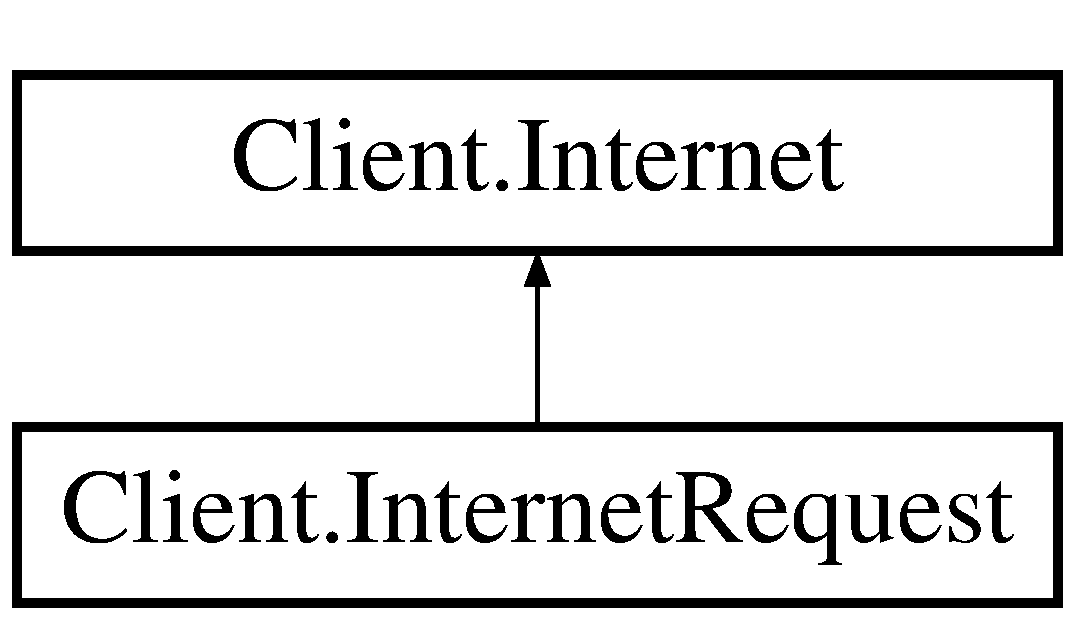
\includegraphics[height=2.000000cm]{class_client_1_1_internet_request}
\end{center}
\end{figure}
\subsection*{Public Member Functions}
\begin{DoxyCompactItemize}
\item 
\hyperlink{class_client_1_1_internet_request_a954431ce4c7f20d28a05158ab3238714}{Internet\+Request} (int Now\+Time, int limit, string sign)
\begin{DoxyCompactList}\small\item\em Строка запросов для получения котировок \end{DoxyCompactList}\item 
Match\+Collection \hyperlink{class_client_1_1_internet_request_aba2389a5a186697ed6eb3ed23edac309}{Internet\+Data} ()
\begin{DoxyCompactList}\small\item\em Парсинг и запрос данных на сервер \end{DoxyCompactList}\end{DoxyCompactItemize}


\subsection{Detailed Description}
Класс интернет запрос 



\subsection{Constructor \& Destructor Documentation}
\hypertarget{class_client_1_1_internet_request_a954431ce4c7f20d28a05158ab3238714}{}\label{class_client_1_1_internet_request_a954431ce4c7f20d28a05158ab3238714} 
\index{Client\+::\+Internet\+Request@{Client\+::\+Internet\+Request}!Internet\+Request@{Internet\+Request}}
\index{Internet\+Request@{Internet\+Request}!Client\+::\+Internet\+Request@{Client\+::\+Internet\+Request}}
\subsubsection{\texorpdfstring{Internet\+Request()}{InternetRequest()}}
{\footnotesize\ttfamily Client.\+Internet\+Request.\+Internet\+Request (\begin{DoxyParamCaption}\item[{int}]{Now\+Time,  }\item[{int}]{limit,  }\item[{string}]{sign }\end{DoxyParamCaption})\hspace{0.3cm}{\ttfamily [inline]}}



Строка запросов для получения котировок 


\begin{DoxyParams}{Parameters}
{\em Now\+Time;} & Текущее время\\
\hline
{\em limit;} & Количество \\
\hline
{\em sign} & Валюта\\
\hline
\end{DoxyParams}


\subsection{Member Function Documentation}
\hypertarget{class_client_1_1_internet_request_aba2389a5a186697ed6eb3ed23edac309}{}\label{class_client_1_1_internet_request_aba2389a5a186697ed6eb3ed23edac309} 
\index{Client\+::\+Internet\+Request@{Client\+::\+Internet\+Request}!Internet\+Data@{Internet\+Data}}
\index{Internet\+Data@{Internet\+Data}!Client\+::\+Internet\+Request@{Client\+::\+Internet\+Request}}
\subsubsection{\texorpdfstring{Internet\+Data()}{InternetData()}}
{\footnotesize\ttfamily Match\+Collection Client.\+Internet\+Request.\+Internet\+Data (\begin{DoxyParamCaption}{ }\end{DoxyParamCaption})\hspace{0.3cm}{\ttfamily [inline]}}



Парсинг и запрос данных на сервер 



The documentation for this class was generated from the following file\+:\begin{DoxyCompactItemize}
\item 
C\+:/\+Users/саша/\+Documents/\+Visual Studio 2015/\+Projects/\+Forex2.\+0/\+Client/Internet\+Request.\+cs\end{DoxyCompactItemize}

\hypertarget{class_client_1_1_interval_resistance}{}\section{Client.\+Interval\+Resistance Class Reference}
\label{class_client_1_1_interval_resistance}\index{Client.\+Interval\+Resistance@{Client.\+Interval\+Resistance}}


Класс формирующий интервалы линии сопротивления  


\subsection*{Public Member Functions}
\begin{DoxyCompactItemize}
\item 
\hyperlink{class_client_1_1_interval_resistance_a106fc4512710179f67ae06bb59dd1082}{Interval\+Resistance} (int tic, List$<$ double $>$ Buffer, double Now\+Time)
\begin{DoxyCompactList}\small\item\em Подавать интервал + \end{DoxyCompactList}\end{DoxyCompactItemize}
\subsection*{Public Attributes}
\begin{DoxyCompactItemize}
\item 
\hypertarget{class_client_1_1_interval_resistance_a951beb2736070f6f01825b07f2c56b60}{}\label{class_client_1_1_interval_resistance_a951beb2736070f6f01825b07f2c56b60} 
int {\bfseries danoe} = 0
\item 
\hypertarget{class_client_1_1_interval_resistance_aa5785984b2dafd978672ac294d5e3add}{}\label{class_client_1_1_interval_resistance_aa5785984b2dafd978672ac294d5e3add} 
List$<$ List$<$ double $>$ $>$ {\bfseries poin} = new List$<$List$<$double$>$$>$()
\end{DoxyCompactItemize}


\subsection{Detailed Description}
Класс формирующий интервалы линии сопротивления 



\subsection{Constructor \& Destructor Documentation}
\hypertarget{class_client_1_1_interval_resistance_a106fc4512710179f67ae06bb59dd1082}{}\label{class_client_1_1_interval_resistance_a106fc4512710179f67ae06bb59dd1082} 
\index{Client\+::\+Interval\+Resistance@{Client\+::\+Interval\+Resistance}!Interval\+Resistance@{Interval\+Resistance}}
\index{Interval\+Resistance@{Interval\+Resistance}!Client\+::\+Interval\+Resistance@{Client\+::\+Interval\+Resistance}}
\subsubsection{\texorpdfstring{Interval\+Resistance()}{IntervalResistance()}}
{\footnotesize\ttfamily Client.\+Interval\+Resistance.\+Interval\+Resistance (\begin{DoxyParamCaption}\item[{int}]{tic,  }\item[{List$<$ double $>$}]{Buffer,  }\item[{double}]{Now\+Time }\end{DoxyParamCaption})\hspace{0.3cm}{\ttfamily [inline]}}



Подавать интервал + 


\begin{DoxyParams}{Parameters}
{\em tic} & время прошедшее с запуска\\
\hline
{\em Buff} & ???\\
\hline
{\em Now\+Time} & Текущее время\\
\hline
\end{DoxyParams}


The documentation for this class was generated from the following file\+:\begin{DoxyCompactItemize}
\item 
C\+:/\+Users/саша/\+Documents/\+Visual Studio 2015/\+Projects/\+Forex2.\+0/\+Client/Interval\+Resistence.\+cs\end{DoxyCompactItemize}

\hypertarget{class_client_1_1_line_coord}{}\section{Client.\+Line\+Coord Class Reference}
\label{class_client_1_1_line_coord}\index{Client.\+Line\+Coord@{Client.\+Line\+Coord}}


Класс отвечающий за координатные линии  


\subsection*{Public Member Functions}
\begin{DoxyCompactItemize}
\item 
\hyperlink{class_client_1_1_line_coord_a0cbce126477bfbcd61f7f717bdc0f5fd}{Line\+Coord} (int x, int y, double fX, double fy, Label lab\+\_\+\+Cur, Label label\+\_\+Y, Label label\+\_\+X, ref Chart graphic)
\begin{DoxyCompactList}\small\item\em Конструктор для линий и лабел + \end{DoxyCompactList}\item 
void \hyperlink{class_client_1_1_line_coord_a4009afb548e23a911cae4238935d8f07}{Ob\+Linecoord} (Label lab\+\_\+\+Cur, Label label\+\_\+Y, Label label\+\_\+X, ref Chart graphic)
\begin{DoxyCompactList}\small\item\em Присвоение лабел и чарт + \end{DoxyCompactList}\item 
void \hyperlink{class_client_1_1_line_coord_a5fdd32f8f5936850de0e1a0836914468}{size\+Line\+Coord} (int x, int y, double fX, double fy)
\begin{DoxyCompactList}\small\item\em Подстраивание размеров под экран + \end{DoxyCompactList}\item 
void \hyperlink{class_client_1_1_line_coord_a8092ccedc304ed8cecfb386016efe877}{Show} (Check\+Box check\+Box\+Line\+Coord)
\begin{DoxyCompactList}\small\item\em Проверка активации чек бокса и отображение линий + \end{DoxyCompactList}\item 
void \hyperlink{class_client_1_1_line_coord_a525dfa0064c415a6317312e7fcfae88f}{chart1\+\_\+\+Mouse\+Move} (object sender, Mouse\+Event\+Args e)
\begin{DoxyCompactList}\small\item\em Событие отвечающие за наведение мыши с помощью линий \end{DoxyCompactList}\end{DoxyCompactItemize}
\subsection*{Properties}
\begin{DoxyCompactItemize}
\item 
double \hyperlink{class_client_1_1_line_coord_a8008869c1c2c60c6d1236f80200c383e}{Svoistvo\+\_\+xS}\hspace{0.3cm}{\ttfamily  \mbox{[}get, set\mbox{]}}
\begin{DoxyCompactList}\small\item\em свойство размеры экрана по икс x \end{DoxyCompactList}\item 
double \hyperlink{class_client_1_1_line_coord_a71bf6f4176e9f7becd572f44f1d4948f}{Svoistvo\+\_\+yS}\hspace{0.3cm}{\ttfamily  \mbox{[}get, set\mbox{]}}
\begin{DoxyCompactList}\small\item\em свойство размеры экрана по икс y \end{DoxyCompactList}\item 
\hypertarget{class_client_1_1_line_coord_a3c39c4ced2b59ddbe0ab9960a456bf72}{}\label{class_client_1_1_line_coord_a3c39c4ced2b59ddbe0ab9960a456bf72} 
double {\bfseries Svoistvo\+\_\+fX}\hspace{0.3cm}{\ttfamily  \mbox{[}get, set\mbox{]}}
\item 
\hypertarget{class_client_1_1_line_coord_a830f017bd6a6606bc5efd1515cf3fc97}{}\label{class_client_1_1_line_coord_a830f017bd6a6606bc5efd1515cf3fc97} 
double {\bfseries Svoistvo\+\_\+fY}\hspace{0.3cm}{\ttfamily  \mbox{[}get, set\mbox{]}}
\item 
Label \hyperlink{class_client_1_1_line_coord_ab896e31d73c3bd32bbec4c389b075f19}{Svoistvo\+\_\+label\+\_\+X}\hspace{0.3cm}{\ttfamily  \mbox{[}get, set\mbox{]}}
\begin{DoxyCompactList}\small\item\em свойство линии по x \end{DoxyCompactList}\item 
Label \hyperlink{class_client_1_1_line_coord_a78a8315868d88677c9780a1025bfc604}{Svoistvo\+\_\+label\+\_\+Y}\hspace{0.3cm}{\ttfamily  \mbox{[}get, set\mbox{]}}
\begin{DoxyCompactList}\small\item\em свойство линии по y \end{DoxyCompactList}\item 
Label \hyperlink{class_client_1_1_line_coord_a419f0d51c6a6ab8755f5313acf10edd7}{Svoistvo\+\_\+lab\+\_\+\+Cur}\hspace{0.3cm}{\ttfamily  \mbox{[}get, set\mbox{]}}
\begin{DoxyCompactList}\small\item\em свойство линии отображающей данные \end{DoxyCompactList}\item 
Chart \hyperlink{class_client_1_1_line_coord_ade37bc49a7a9e2daaec818e4dd3a275f}{Svoistvo\+\_\+graphic}\hspace{0.3cm}{\ttfamily  \mbox{[}get, set\mbox{]}}
\begin{DoxyCompactList}\small\item\em свойство график \end{DoxyCompactList}\end{DoxyCompactItemize}


\subsection{Detailed Description}
Класс отвечающий за координатные линии 



\subsection{Constructor \& Destructor Documentation}
\hypertarget{class_client_1_1_line_coord_a0cbce126477bfbcd61f7f717bdc0f5fd}{}\label{class_client_1_1_line_coord_a0cbce126477bfbcd61f7f717bdc0f5fd} 
\index{Client\+::\+Line\+Coord@{Client\+::\+Line\+Coord}!Line\+Coord@{Line\+Coord}}
\index{Line\+Coord@{Line\+Coord}!Client\+::\+Line\+Coord@{Client\+::\+Line\+Coord}}
\subsubsection{\texorpdfstring{Line\+Coord()}{LineCoord()}}
{\footnotesize\ttfamily Client.\+Line\+Coord.\+Line\+Coord (\begin{DoxyParamCaption}\item[{int}]{x,  }\item[{int}]{y,  }\item[{double}]{fX,  }\item[{double}]{fy,  }\item[{Label}]{lab\+\_\+\+Cur,  }\item[{Label}]{label\+\_\+Y,  }\item[{Label}]{label\+\_\+X,  }\item[{ref Chart}]{graphic }\end{DoxyParamCaption})\hspace{0.3cm}{\ttfamily [inline]}}



Конструктор для линий и лабел + 


\begin{DoxyParams}{Parameters}
{\em x} & размеры экрана по икс\\
\hline
{\em y} & размеры экрана по игрик\\
\hline
{\em fy} & \\
\hline
{\em fx} & \\
\hline
{\em lab\+\_\+\+Cur} & Курс в точке\\
\hline
{\em label\+\_\+Y} & Линия по Y\\
\hline
{\em label\+\_\+X} & Линия по X\\
\hline
{\em graphic} & Chart\\
\hline
\end{DoxyParams}


\subsection{Member Function Documentation}
\hypertarget{class_client_1_1_line_coord_a525dfa0064c415a6317312e7fcfae88f}{}\label{class_client_1_1_line_coord_a525dfa0064c415a6317312e7fcfae88f} 
\index{Client\+::\+Line\+Coord@{Client\+::\+Line\+Coord}!chart1\+\_\+\+Mouse\+Move@{chart1\+\_\+\+Mouse\+Move}}
\index{chart1\+\_\+\+Mouse\+Move@{chart1\+\_\+\+Mouse\+Move}!Client\+::\+Line\+Coord@{Client\+::\+Line\+Coord}}
\subsubsection{\texorpdfstring{chart1\+\_\+\+Mouse\+Move()}{chart1\_MouseMove()}}
{\footnotesize\ttfamily void Client.\+Line\+Coord.\+chart1\+\_\+\+Mouse\+Move (\begin{DoxyParamCaption}\item[{object}]{sender,  }\item[{Mouse\+Event\+Args}]{e }\end{DoxyParamCaption})\hspace{0.3cm}{\ttfamily [inline]}}



Событие отвечающие за наведение мыши с помощью линий 


\begin{DoxyParams}{Parameters}
{\em e} & чек бокс отвечающий за активацию линий\\
\hline
{\em sender} & чек бокс отвечающий за активацию линий\\
\hline
\end{DoxyParams}
\hypertarget{class_client_1_1_line_coord_a4009afb548e23a911cae4238935d8f07}{}\label{class_client_1_1_line_coord_a4009afb548e23a911cae4238935d8f07} 
\index{Client\+::\+Line\+Coord@{Client\+::\+Line\+Coord}!Ob\+Linecoord@{Ob\+Linecoord}}
\index{Ob\+Linecoord@{Ob\+Linecoord}!Client\+::\+Line\+Coord@{Client\+::\+Line\+Coord}}
\subsubsection{\texorpdfstring{Ob\+Linecoord()}{ObLinecoord()}}
{\footnotesize\ttfamily void Client.\+Line\+Coord.\+Ob\+Linecoord (\begin{DoxyParamCaption}\item[{Label}]{lab\+\_\+\+Cur,  }\item[{Label}]{label\+\_\+Y,  }\item[{Label}]{label\+\_\+X,  }\item[{ref Chart}]{graphic }\end{DoxyParamCaption})\hspace{0.3cm}{\ttfamily [inline]}}



Присвоение лабел и чарт + 


\begin{DoxyParams}{Parameters}
{\em lab\+\_\+\+Cur} & Курс в точке\\
\hline
{\em label\+\_\+Y} & Линия по Y\\
\hline
{\em label\+\_\+X} & Линия по X\\
\hline
{\em graphic} & Chart\\
\hline
\end{DoxyParams}
\hypertarget{class_client_1_1_line_coord_a8092ccedc304ed8cecfb386016efe877}{}\label{class_client_1_1_line_coord_a8092ccedc304ed8cecfb386016efe877} 
\index{Client\+::\+Line\+Coord@{Client\+::\+Line\+Coord}!Show@{Show}}
\index{Show@{Show}!Client\+::\+Line\+Coord@{Client\+::\+Line\+Coord}}
\subsubsection{\texorpdfstring{Show()}{Show()}}
{\footnotesize\ttfamily void Client.\+Line\+Coord.\+Show (\begin{DoxyParamCaption}\item[{Check\+Box}]{check\+Box\+Line\+Coord }\end{DoxyParamCaption})\hspace{0.3cm}{\ttfamily [inline]}}



Проверка активации чек бокса и отображение линий + 


\begin{DoxyParams}{Parameters}
{\em check\+Box\+Line\+Coord} & чек бокс отвечающий за активацию линий\\
\hline
\end{DoxyParams}
\hypertarget{class_client_1_1_line_coord_a5fdd32f8f5936850de0e1a0836914468}{}\label{class_client_1_1_line_coord_a5fdd32f8f5936850de0e1a0836914468} 
\index{Client\+::\+Line\+Coord@{Client\+::\+Line\+Coord}!size\+Line\+Coord@{size\+Line\+Coord}}
\index{size\+Line\+Coord@{size\+Line\+Coord}!Client\+::\+Line\+Coord@{Client\+::\+Line\+Coord}}
\subsubsection{\texorpdfstring{size\+Line\+Coord()}{sizeLineCoord()}}
{\footnotesize\ttfamily void Client.\+Line\+Coord.\+size\+Line\+Coord (\begin{DoxyParamCaption}\item[{int}]{x,  }\item[{int}]{y,  }\item[{double}]{fX,  }\item[{double}]{fy }\end{DoxyParamCaption})\hspace{0.3cm}{\ttfamily [inline]}}



Подстраивание размеров под экран + 


\begin{DoxyParams}{Parameters}
{\em x} & размеры экрана по икс\\
\hline
{\em y} & размеры экрана по игрик\\
\hline
{\em fy} & \\
\hline
{\em fx} & \\
\hline
\end{DoxyParams}


\subsection{Property Documentation}
\hypertarget{class_client_1_1_line_coord_ade37bc49a7a9e2daaec818e4dd3a275f}{}\label{class_client_1_1_line_coord_ade37bc49a7a9e2daaec818e4dd3a275f} 
\index{Client\+::\+Line\+Coord@{Client\+::\+Line\+Coord}!Svoistvo\+\_\+graphic@{Svoistvo\+\_\+graphic}}
\index{Svoistvo\+\_\+graphic@{Svoistvo\+\_\+graphic}!Client\+::\+Line\+Coord@{Client\+::\+Line\+Coord}}
\subsubsection{\texorpdfstring{Svoistvo\+\_\+graphic}{Svoistvo\_graphic}}
{\footnotesize\ttfamily Chart Client.\+Line\+Coord.\+Svoistvo\+\_\+graphic\hspace{0.3cm}{\ttfamily [get]}, {\ttfamily [set]}}



свойство график 

\hypertarget{class_client_1_1_line_coord_a419f0d51c6a6ab8755f5313acf10edd7}{}\label{class_client_1_1_line_coord_a419f0d51c6a6ab8755f5313acf10edd7} 
\index{Client\+::\+Line\+Coord@{Client\+::\+Line\+Coord}!Svoistvo\+\_\+lab\+\_\+\+Cur@{Svoistvo\+\_\+lab\+\_\+\+Cur}}
\index{Svoistvo\+\_\+lab\+\_\+\+Cur@{Svoistvo\+\_\+lab\+\_\+\+Cur}!Client\+::\+Line\+Coord@{Client\+::\+Line\+Coord}}
\subsubsection{\texorpdfstring{Svoistvo\+\_\+lab\+\_\+\+Cur}{Svoistvo\_lab\_Cur}}
{\footnotesize\ttfamily Label Client.\+Line\+Coord.\+Svoistvo\+\_\+lab\+\_\+\+Cur\hspace{0.3cm}{\ttfamily [get]}, {\ttfamily [set]}}



свойство линии отображающей данные 

\hypertarget{class_client_1_1_line_coord_ab896e31d73c3bd32bbec4c389b075f19}{}\label{class_client_1_1_line_coord_ab896e31d73c3bd32bbec4c389b075f19} 
\index{Client\+::\+Line\+Coord@{Client\+::\+Line\+Coord}!Svoistvo\+\_\+label\+\_\+X@{Svoistvo\+\_\+label\+\_\+X}}
\index{Svoistvo\+\_\+label\+\_\+X@{Svoistvo\+\_\+label\+\_\+X}!Client\+::\+Line\+Coord@{Client\+::\+Line\+Coord}}
\subsubsection{\texorpdfstring{Svoistvo\+\_\+label\+\_\+X}{Svoistvo\_label\_X}}
{\footnotesize\ttfamily Label Client.\+Line\+Coord.\+Svoistvo\+\_\+label\+\_\+X\hspace{0.3cm}{\ttfamily [get]}, {\ttfamily [set]}}



свойство линии по x 

\hypertarget{class_client_1_1_line_coord_a78a8315868d88677c9780a1025bfc604}{}\label{class_client_1_1_line_coord_a78a8315868d88677c9780a1025bfc604} 
\index{Client\+::\+Line\+Coord@{Client\+::\+Line\+Coord}!Svoistvo\+\_\+label\+\_\+Y@{Svoistvo\+\_\+label\+\_\+Y}}
\index{Svoistvo\+\_\+label\+\_\+Y@{Svoistvo\+\_\+label\+\_\+Y}!Client\+::\+Line\+Coord@{Client\+::\+Line\+Coord}}
\subsubsection{\texorpdfstring{Svoistvo\+\_\+label\+\_\+Y}{Svoistvo\_label\_Y}}
{\footnotesize\ttfamily Label Client.\+Line\+Coord.\+Svoistvo\+\_\+label\+\_\+Y\hspace{0.3cm}{\ttfamily [get]}, {\ttfamily [set]}}



свойство линии по y 

\hypertarget{class_client_1_1_line_coord_a8008869c1c2c60c6d1236f80200c383e}{}\label{class_client_1_1_line_coord_a8008869c1c2c60c6d1236f80200c383e} 
\index{Client\+::\+Line\+Coord@{Client\+::\+Line\+Coord}!Svoistvo\+\_\+xS@{Svoistvo\+\_\+xS}}
\index{Svoistvo\+\_\+xS@{Svoistvo\+\_\+xS}!Client\+::\+Line\+Coord@{Client\+::\+Line\+Coord}}
\subsubsection{\texorpdfstring{Svoistvo\+\_\+xS}{Svoistvo\_xS}}
{\footnotesize\ttfamily double Client.\+Line\+Coord.\+Svoistvo\+\_\+xS\hspace{0.3cm}{\ttfamily [get]}, {\ttfamily [set]}}



свойство размеры экрана по икс x 

\hypertarget{class_client_1_1_line_coord_a71bf6f4176e9f7becd572f44f1d4948f}{}\label{class_client_1_1_line_coord_a71bf6f4176e9f7becd572f44f1d4948f} 
\index{Client\+::\+Line\+Coord@{Client\+::\+Line\+Coord}!Svoistvo\+\_\+yS@{Svoistvo\+\_\+yS}}
\index{Svoistvo\+\_\+yS@{Svoistvo\+\_\+yS}!Client\+::\+Line\+Coord@{Client\+::\+Line\+Coord}}
\subsubsection{\texorpdfstring{Svoistvo\+\_\+yS}{Svoistvo\_yS}}
{\footnotesize\ttfamily double Client.\+Line\+Coord.\+Svoistvo\+\_\+yS\hspace{0.3cm}{\ttfamily [get]}, {\ttfamily [set]}}



свойство размеры экрана по икс y 



The documentation for this class was generated from the following file\+:\begin{DoxyCompactItemize}
\item 
C\+:/\+Users/саша/\+Documents/\+Visual Studio 2015/\+Projects/\+Forex2.\+0/\+Client/Line\+Coord.\+cs\end{DoxyCompactItemize}

\hypertarget{class_client_1_1_main_form}{}\section{Client.\+Main\+Form Class Reference}
\label{class_client_1_1_main_form}\index{Client.\+Main\+Form@{Client.\+Main\+Form}}


Стартовое окно  


Inheritance diagram for Client.\+Main\+Form\+:\begin{figure}[H]
\begin{center}
\leavevmode
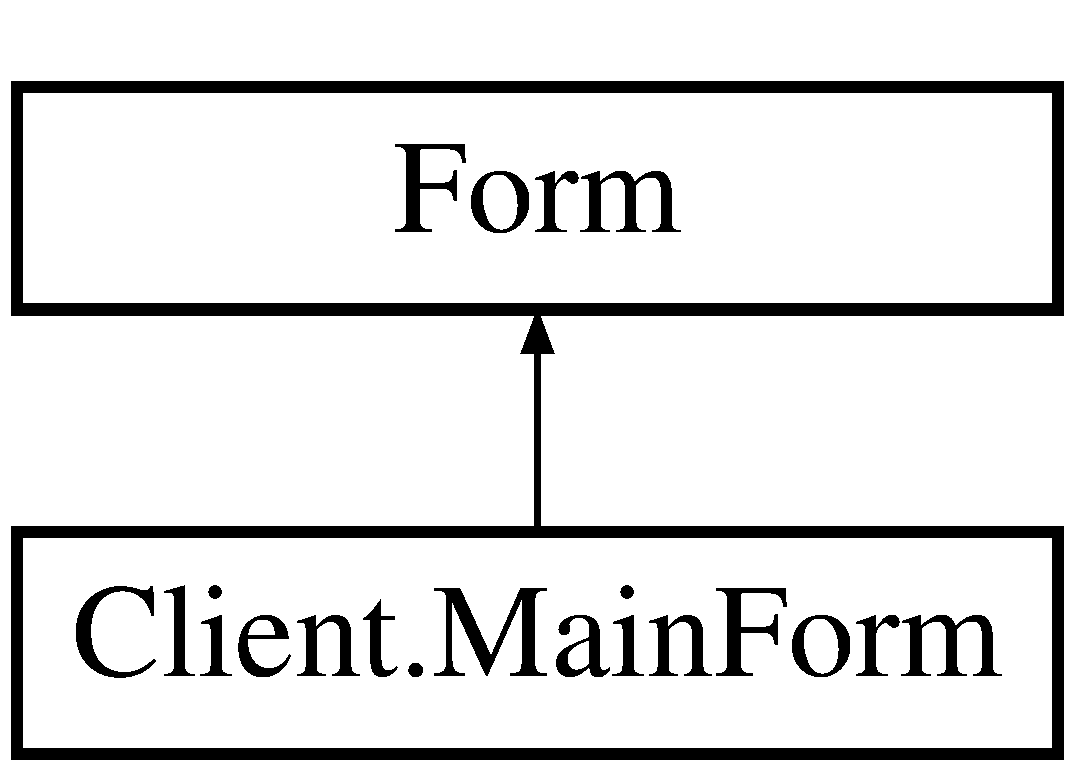
\includegraphics[height=2.000000cm]{class_client_1_1_main_form}
\end{center}
\end{figure}
\subsection*{Public Member Functions}
\begin{DoxyCompactItemize}
\item 
\hyperlink{class_client_1_1_main_form_a67c808fc65fba26e70e1e36dc083d131}{Main\+Form} (int x, int y)
\begin{DoxyCompactList}\small\item\em Конструктор стартового состояния окна \end{DoxyCompactList}\item 
void \hyperlink{class_client_1_1_main_form_a3200a9b853b787c11bc1fa2e974e472b}{write\+File} (string path\+File)
\begin{DoxyCompactList}\small\item\em Конструктор стартового состояния окна \end{DoxyCompactList}\item 
void \hyperlink{class_client_1_1_main_form_a736b03fd5ca2af0171db525573891553}{E\+U\+R\+U\+S\+D\+Tool\+Strip\+Menu\+Item\+\_\+\+Click} (object sender, Event\+Args e)
\begin{DoxyCompactList}\small\item\em Cоздание окна \end{DoxyCompactList}\item 
void \hyperlink{class_client_1_1_main_form_ae422739b1b0042a9b697ea2c446ac7c5}{U\+S\+D\+J\+P\+Y\+Tool\+Strip\+Menu\+Item\+\_\+\+Click} (object sender, Event\+Args e)
\begin{DoxyCompactList}\small\item\em Cоздание окна \end{DoxyCompactList}\item 
bool \hyperlink{class_client_1_1_main_form_acdcf3f02f06d2f0256c0d93411c6d4b1}{create\+Window} (Task T\+Qoute, bool close\+Window, string value)
\begin{DoxyCompactList}\small\item\em Метод для создания окна котировок \end{DoxyCompactList}\item 
bool \hyperlink{class_client_1_1_main_form_a48f67f872cf157e9be746823e1cba8e8}{Tasks} (Task t\+Connect, Task t\+Loadquotes)
\begin{DoxyCompactList}\small\item\em Ожидание загрузки данных \end{DoxyCompactList}\item 
void \hyperlink{class_client_1_1_main_form_a9356e4f0bb6127a253382090bdca5707}{Window\+Size\+Location} (\hyperlink{class_client_1_1_windowd}{Windowd} quotes\+Window, int sizeX, int sizeY)
\begin{DoxyCompactList}\small\item\em Метод для установки окну параметра Mdi\+Parent, скрытия контейнера, показ окна, и сохранение в хранилище окон \end{DoxyCompactList}\item 
void \hyperlink{class_client_1_1_main_form_a1c104c0cc622e2a763915c5d7500a515}{Window\+Tool\+Strip\+Menu\+Item\+\_\+\+Click} (object sender, Event\+Args e)
\begin{DoxyCompactList}\small\item\em Создание окна \hyperlink{class_client_1_1_s_window}{S\+Window} \end{DoxyCompactList}\item 
void \hyperlink{class_client_1_1_main_form_ae2d7d0d2a2ce5e8495d2e17e162e5506}{Help\+Tool\+Strip\+Menu\+Item\+\_\+\+Click} (object sender, Event\+Args e)
\begin{DoxyCompactList}\small\item\em Создание окна Help\+Closing \end{DoxyCompactList}\item 
void \hyperlink{class_client_1_1_main_form_a0d8831ab5fe970a2196b2ee35bf6508a}{Change\+Text\+Language} ()
\begin{DoxyCompactList}\small\item\em Метод смены языка \end{DoxyCompactList}\item 
\hypertarget{class_client_1_1_main_form_a5c23c1a74e8fc0090620434ee71ff10c}{}\label{class_client_1_1_main_form_a5c23c1a74e8fc0090620434ee71ff10c} 
void {\bfseries Edit\+Interface} (string settings\+Tool\+Strip\+Menu, string window\+Tool\+Strip\+Menu, string chart\+Tool\+Strip\+Menu, string About\+Tool\+Strip\+Menu, string Tool\+Strip\+Menu, string help\+Tool\+Strip\+Menu, string currency\+Pairs\+Tool\+Strip\+Menu, string e\+U\+R\+U\+S\+D\+Tool\+Strip\+Menu, string U\+S\+D\+J\+P\+Y\+Tool\+Strip\+Menu, string lang\+Tool\+Strip\+Menu, string label\+Select)
\end{DoxyCompactItemize}
\subsection*{Public Attributes}
\begin{DoxyCompactItemize}
\item 
\hypertarget{class_client_1_1_main_form_af9bb38bbfa2d759792f533061cf7d17a}{}\label{class_client_1_1_main_form_af9bb38bbfa2d759792f533061cf7d17a} 
List$<$ string $>$ {\bfseries valueP} = new List$<$string$>$()
\item 
List$<$ \hyperlink{class_client_1_1_windowd}{Windowd} $>$ \hyperlink{class_client_1_1_main_form_a3e3dca9d63d0282147f521d7f209444f}{windows} = new List$<$\hyperlink{class_client_1_1_windowd}{Windowd}$>$()
\begin{DoxyCompactList}\small\item\em реализация окна валюты \end{DoxyCompactList}\end{DoxyCompactItemize}
\subsection*{Static Public Attributes}
\begin{DoxyCompactItemize}
\item 
static bool \hyperlink{class_client_1_1_main_form_af46e70fe2775cc145de943ab8b152075}{Help\+Closing} = true
\begin{DoxyCompactList}\small\item\em поле отвечающая за закрытое окной \hyperlink{class_client_1_1_help}{Help} \end{DoxyCompactList}\item 
static bool \hyperlink{class_client_1_1_main_form_a623ae96ca11ba63ec5ecb191edf2fab0}{S\+Window\+Closing} = true
\begin{DoxyCompactList}\small\item\em поле отвечающая за закрытое окной \hyperlink{class_client_1_1_s_window}{S\+Window} \end{DoxyCompactList}\item 
static bool \hyperlink{class_client_1_1_main_form_af628f3dc899c945ef7347506f4c5612f}{Window\+Closing\+E\+U\+R\+U\+SD} = true
\begin{DoxyCompactList}\small\item\em поле отвечающая за закрытое окной Window \end{DoxyCompactList}\item 
static bool \hyperlink{class_client_1_1_main_form_a803bcf3080d58c8bcabb930e01193d09}{Window\+Closing\+U\+S\+D\+J\+PY} = true
\begin{DoxyCompactList}\small\item\em поле отвечающая за закрытое окной U\+S\+D\+J\+PY \end{DoxyCompactList}\item 
static bool \hyperlink{class_client_1_1_main_form_aa9598c4369dac295d4c45455ca7133f4}{S\+Chart\+Closing} = true
\begin{DoxyCompactList}\small\item\em поле отвечающая за закрытое окной S\+Char \end{DoxyCompactList}\end{DoxyCompactItemize}
\subsection*{Protected Member Functions}
\begin{DoxyCompactItemize}
\item 
override void \hyperlink{class_client_1_1_main_form_a50155117b57f40079e26d88695114488}{Dispose} (bool disposing)
\begin{DoxyCompactList}\small\item\em Освободить все используемые ресурсы. \end{DoxyCompactList}\end{DoxyCompactItemize}


\subsection{Detailed Description}
Стартовое окно 



\subsection{Constructor \& Destructor Documentation}
\hypertarget{class_client_1_1_main_form_a67c808fc65fba26e70e1e36dc083d131}{}\label{class_client_1_1_main_form_a67c808fc65fba26e70e1e36dc083d131} 
\index{Client\+::\+Main\+Form@{Client\+::\+Main\+Form}!Main\+Form@{Main\+Form}}
\index{Main\+Form@{Main\+Form}!Client\+::\+Main\+Form@{Client\+::\+Main\+Form}}
\subsubsection{\texorpdfstring{Main\+Form()}{MainForm()}}
{\footnotesize\ttfamily Client.\+Main\+Form.\+Main\+Form (\begin{DoxyParamCaption}\item[{int}]{x,  }\item[{int}]{y }\end{DoxyParamCaption})\hspace{0.3cm}{\ttfamily [inline]}}



Конструктор стартового состояния окна 


\begin{DoxyParams}{Parameters}
{\em x} & размер по оси x\\
\hline
{\em y} & размер по оси y\\
\hline
\end{DoxyParams}


\subsection{Member Function Documentation}
\hypertarget{class_client_1_1_main_form_a0d8831ab5fe970a2196b2ee35bf6508a}{}\label{class_client_1_1_main_form_a0d8831ab5fe970a2196b2ee35bf6508a} 
\index{Client\+::\+Main\+Form@{Client\+::\+Main\+Form}!Change\+Text\+Language@{Change\+Text\+Language}}
\index{Change\+Text\+Language@{Change\+Text\+Language}!Client\+::\+Main\+Form@{Client\+::\+Main\+Form}}
\subsubsection{\texorpdfstring{Change\+Text\+Language()}{ChangeTextLanguage()}}
{\footnotesize\ttfamily void Client.\+Main\+Form.\+Change\+Text\+Language (\begin{DoxyParamCaption}{ }\end{DoxyParamCaption})\hspace{0.3cm}{\ttfamily [inline]}}



Метод смены языка 

\hypertarget{class_client_1_1_main_form_acdcf3f02f06d2f0256c0d93411c6d4b1}{}\label{class_client_1_1_main_form_acdcf3f02f06d2f0256c0d93411c6d4b1} 
\index{Client\+::\+Main\+Form@{Client\+::\+Main\+Form}!create\+Window@{create\+Window}}
\index{create\+Window@{create\+Window}!Client\+::\+Main\+Form@{Client\+::\+Main\+Form}}
\subsubsection{\texorpdfstring{create\+Window()}{createWindow()}}
{\footnotesize\ttfamily bool Client.\+Main\+Form.\+create\+Window (\begin{DoxyParamCaption}\item[{Task}]{T\+Qoute,  }\item[{bool}]{close\+Window,  }\item[{string}]{value }\end{DoxyParamCaption})\hspace{0.3cm}{\ttfamily [inline]}}



Метод для создания окна котировок 


\begin{DoxyParams}{Parameters}
{\em t\+Connect} & Таск подключения\\
\hline
{\em t\+Loadquotes} & Таск погрузки данных\\
\hline
{\em close\+Window} & \\
\hline
\end{DoxyParams}
param name=\char`\"{}value\char`\"{}$>$наименование котировки\hypertarget{class_client_1_1_main_form_a50155117b57f40079e26d88695114488}{}\label{class_client_1_1_main_form_a50155117b57f40079e26d88695114488} 
\index{Client\+::\+Main\+Form@{Client\+::\+Main\+Form}!Dispose@{Dispose}}
\index{Dispose@{Dispose}!Client\+::\+Main\+Form@{Client\+::\+Main\+Form}}
\subsubsection{\texorpdfstring{Dispose()}{Dispose()}}
{\footnotesize\ttfamily override void Client.\+Main\+Form.\+Dispose (\begin{DoxyParamCaption}\item[{bool}]{disposing }\end{DoxyParamCaption})\hspace{0.3cm}{\ttfamily [inline]}, {\ttfamily [protected]}}



Освободить все используемые ресурсы. 


\begin{DoxyParams}{Parameters}
{\em disposing} & истинно, если управляемый ресурс должен быть удален; иначе ложно.\\
\hline
\end{DoxyParams}
\hypertarget{class_client_1_1_main_form_a736b03fd5ca2af0171db525573891553}{}\label{class_client_1_1_main_form_a736b03fd5ca2af0171db525573891553} 
\index{Client\+::\+Main\+Form@{Client\+::\+Main\+Form}!E\+U\+R\+U\+S\+D\+Tool\+Strip\+Menu\+Item\+\_\+\+Click@{E\+U\+R\+U\+S\+D\+Tool\+Strip\+Menu\+Item\+\_\+\+Click}}
\index{E\+U\+R\+U\+S\+D\+Tool\+Strip\+Menu\+Item\+\_\+\+Click@{E\+U\+R\+U\+S\+D\+Tool\+Strip\+Menu\+Item\+\_\+\+Click}!Client\+::\+Main\+Form@{Client\+::\+Main\+Form}}
\subsubsection{\texorpdfstring{E\+U\+R\+U\+S\+D\+Tool\+Strip\+Menu\+Item\+\_\+\+Click()}{EURUSDToolStripMenuItem\_Click()}}
{\footnotesize\ttfamily void Client.\+Main\+Form.\+E\+U\+R\+U\+S\+D\+Tool\+Strip\+Menu\+Item\+\_\+\+Click (\begin{DoxyParamCaption}\item[{object}]{sender,  }\item[{Event\+Args}]{e }\end{DoxyParamCaption})\hspace{0.3cm}{\ttfamily [inline]}}



Cоздание окна 


\begin{DoxyParams}{Parameters}
{\em sender} & object\\
\hline
{\em e} & Event\+Args\\
\hline
\end{DoxyParams}
\hypertarget{class_client_1_1_main_form_ae2d7d0d2a2ce5e8495d2e17e162e5506}{}\label{class_client_1_1_main_form_ae2d7d0d2a2ce5e8495d2e17e162e5506} 
\index{Client\+::\+Main\+Form@{Client\+::\+Main\+Form}!Help\+Tool\+Strip\+Menu\+Item\+\_\+\+Click@{Help\+Tool\+Strip\+Menu\+Item\+\_\+\+Click}}
\index{Help\+Tool\+Strip\+Menu\+Item\+\_\+\+Click@{Help\+Tool\+Strip\+Menu\+Item\+\_\+\+Click}!Client\+::\+Main\+Form@{Client\+::\+Main\+Form}}
\subsubsection{\texorpdfstring{Help\+Tool\+Strip\+Menu\+Item\+\_\+\+Click()}{HelpToolStripMenuItem\_Click()}}
{\footnotesize\ttfamily void Client.\+Main\+Form.\+Help\+Tool\+Strip\+Menu\+Item\+\_\+\+Click (\begin{DoxyParamCaption}\item[{object}]{sender,  }\item[{Event\+Args}]{e }\end{DoxyParamCaption})\hspace{0.3cm}{\ttfamily [inline]}}



Создание окна Help\+Closing 


\begin{DoxyParams}{Parameters}
{\em sender} & object\\
\hline
{\em e} & Event\+Args\\
\hline
\end{DoxyParams}
\hypertarget{class_client_1_1_main_form_a48f67f872cf157e9be746823e1cba8e8}{}\label{class_client_1_1_main_form_a48f67f872cf157e9be746823e1cba8e8} 
\index{Client\+::\+Main\+Form@{Client\+::\+Main\+Form}!Tasks@{Tasks}}
\index{Tasks@{Tasks}!Client\+::\+Main\+Form@{Client\+::\+Main\+Form}}
\subsubsection{\texorpdfstring{Tasks()}{Tasks()}}
{\footnotesize\ttfamily bool Client.\+Main\+Form.\+Tasks (\begin{DoxyParamCaption}\item[{Task}]{t\+Connect,  }\item[{Task}]{t\+Loadquotes }\end{DoxyParamCaption})\hspace{0.3cm}{\ttfamily [inline]}}



Ожидание загрузки данных 


\begin{DoxyParams}{Parameters}
{\em t\+Connect} & Таск подключения\\
\hline
{\em t\+Loadquotes} & Таск погрузки данных\\
\hline
\end{DoxyParams}
\hypertarget{class_client_1_1_main_form_ae422739b1b0042a9b697ea2c446ac7c5}{}\label{class_client_1_1_main_form_ae422739b1b0042a9b697ea2c446ac7c5} 
\index{Client\+::\+Main\+Form@{Client\+::\+Main\+Form}!U\+S\+D\+J\+P\+Y\+Tool\+Strip\+Menu\+Item\+\_\+\+Click@{U\+S\+D\+J\+P\+Y\+Tool\+Strip\+Menu\+Item\+\_\+\+Click}}
\index{U\+S\+D\+J\+P\+Y\+Tool\+Strip\+Menu\+Item\+\_\+\+Click@{U\+S\+D\+J\+P\+Y\+Tool\+Strip\+Menu\+Item\+\_\+\+Click}!Client\+::\+Main\+Form@{Client\+::\+Main\+Form}}
\subsubsection{\texorpdfstring{U\+S\+D\+J\+P\+Y\+Tool\+Strip\+Menu\+Item\+\_\+\+Click()}{USDJPYToolStripMenuItem\_Click()}}
{\footnotesize\ttfamily void Client.\+Main\+Form.\+U\+S\+D\+J\+P\+Y\+Tool\+Strip\+Menu\+Item\+\_\+\+Click (\begin{DoxyParamCaption}\item[{object}]{sender,  }\item[{Event\+Args}]{e }\end{DoxyParamCaption})\hspace{0.3cm}{\ttfamily [inline]}}



Cоздание окна 


\begin{DoxyParams}{Parameters}
{\em sender} & object\\
\hline
{\em e} & Event\+Args\\
\hline
\end{DoxyParams}
\hypertarget{class_client_1_1_main_form_a9356e4f0bb6127a253382090bdca5707}{}\label{class_client_1_1_main_form_a9356e4f0bb6127a253382090bdca5707} 
\index{Client\+::\+Main\+Form@{Client\+::\+Main\+Form}!Window\+Size\+Location@{Window\+Size\+Location}}
\index{Window\+Size\+Location@{Window\+Size\+Location}!Client\+::\+Main\+Form@{Client\+::\+Main\+Form}}
\subsubsection{\texorpdfstring{Window\+Size\+Location()}{WindowSizeLocation()}}
{\footnotesize\ttfamily void Client.\+Main\+Form.\+Window\+Size\+Location (\begin{DoxyParamCaption}\item[{\hyperlink{class_client_1_1_windowd}{Windowd}}]{quotes\+Window,  }\item[{int}]{sizeX,  }\item[{int}]{sizeY }\end{DoxyParamCaption})\hspace{0.3cm}{\ttfamily [inline]}}



Метод для установки окну параметра Mdi\+Parent, скрытия контейнера, показ окна, и сохранение в хранилище окон 


\begin{DoxyParams}{Parameters}
{\em quotes\+Window} & окно котировок\\
\hline
{\em sizeX} & размеры по X\\
\hline
{\em sizeY} & размеры по Y\\
\hline
\end{DoxyParams}
\hypertarget{class_client_1_1_main_form_a1c104c0cc622e2a763915c5d7500a515}{}\label{class_client_1_1_main_form_a1c104c0cc622e2a763915c5d7500a515} 
\index{Client\+::\+Main\+Form@{Client\+::\+Main\+Form}!Window\+Tool\+Strip\+Menu\+Item\+\_\+\+Click@{Window\+Tool\+Strip\+Menu\+Item\+\_\+\+Click}}
\index{Window\+Tool\+Strip\+Menu\+Item\+\_\+\+Click@{Window\+Tool\+Strip\+Menu\+Item\+\_\+\+Click}!Client\+::\+Main\+Form@{Client\+::\+Main\+Form}}
\subsubsection{\texorpdfstring{Window\+Tool\+Strip\+Menu\+Item\+\_\+\+Click()}{WindowToolStripMenuItem\_Click()}}
{\footnotesize\ttfamily void Client.\+Main\+Form.\+Window\+Tool\+Strip\+Menu\+Item\+\_\+\+Click (\begin{DoxyParamCaption}\item[{object}]{sender,  }\item[{Event\+Args}]{e }\end{DoxyParamCaption})\hspace{0.3cm}{\ttfamily [inline]}}



Создание окна \hyperlink{class_client_1_1_s_window}{S\+Window} 


\begin{DoxyParams}{Parameters}
{\em sender} & object\\
\hline
{\em e} & Event\+Args\\
\hline
\end{DoxyParams}
\hypertarget{class_client_1_1_main_form_a3200a9b853b787c11bc1fa2e974e472b}{}\label{class_client_1_1_main_form_a3200a9b853b787c11bc1fa2e974e472b} 
\index{Client\+::\+Main\+Form@{Client\+::\+Main\+Form}!write\+File@{write\+File}}
\index{write\+File@{write\+File}!Client\+::\+Main\+Form@{Client\+::\+Main\+Form}}
\subsubsection{\texorpdfstring{write\+File()}{writeFile()}}
{\footnotesize\ttfamily void Client.\+Main\+Form.\+write\+File (\begin{DoxyParamCaption}\item[{string}]{path\+File }\end{DoxyParamCaption})\hspace{0.3cm}{\ttfamily [inline]}}



Конструктор стартового состояния окна 


\begin{DoxyParams}{Parameters}
{\em path\+File} & Путь в файл\\
\hline
\end{DoxyParams}


\subsection{Member Data Documentation}
\hypertarget{class_client_1_1_main_form_af46e70fe2775cc145de943ab8b152075}{}\label{class_client_1_1_main_form_af46e70fe2775cc145de943ab8b152075} 
\index{Client\+::\+Main\+Form@{Client\+::\+Main\+Form}!Help\+Closing@{Help\+Closing}}
\index{Help\+Closing@{Help\+Closing}!Client\+::\+Main\+Form@{Client\+::\+Main\+Form}}
\subsubsection{\texorpdfstring{Help\+Closing}{HelpClosing}}
{\footnotesize\ttfamily bool Client.\+Main\+Form.\+Help\+Closing = true\hspace{0.3cm}{\ttfamily [static]}}



поле отвечающая за закрытое окной \hyperlink{class_client_1_1_help}{Help} 

\hypertarget{class_client_1_1_main_form_aa9598c4369dac295d4c45455ca7133f4}{}\label{class_client_1_1_main_form_aa9598c4369dac295d4c45455ca7133f4} 
\index{Client\+::\+Main\+Form@{Client\+::\+Main\+Form}!S\+Chart\+Closing@{S\+Chart\+Closing}}
\index{S\+Chart\+Closing@{S\+Chart\+Closing}!Client\+::\+Main\+Form@{Client\+::\+Main\+Form}}
\subsubsection{\texorpdfstring{S\+Chart\+Closing}{SChartClosing}}
{\footnotesize\ttfamily bool Client.\+Main\+Form.\+S\+Chart\+Closing = true\hspace{0.3cm}{\ttfamily [static]}}



поле отвечающая за закрытое окной S\+Char 

\hypertarget{class_client_1_1_main_form_a623ae96ca11ba63ec5ecb191edf2fab0}{}\label{class_client_1_1_main_form_a623ae96ca11ba63ec5ecb191edf2fab0} 
\index{Client\+::\+Main\+Form@{Client\+::\+Main\+Form}!S\+Window\+Closing@{S\+Window\+Closing}}
\index{S\+Window\+Closing@{S\+Window\+Closing}!Client\+::\+Main\+Form@{Client\+::\+Main\+Form}}
\subsubsection{\texorpdfstring{S\+Window\+Closing}{SWindowClosing}}
{\footnotesize\ttfamily bool Client.\+Main\+Form.\+S\+Window\+Closing = true\hspace{0.3cm}{\ttfamily [static]}}



поле отвечающая за закрытое окной \hyperlink{class_client_1_1_s_window}{S\+Window} 

\hypertarget{class_client_1_1_main_form_af628f3dc899c945ef7347506f4c5612f}{}\label{class_client_1_1_main_form_af628f3dc899c945ef7347506f4c5612f} 
\index{Client\+::\+Main\+Form@{Client\+::\+Main\+Form}!Window\+Closing\+E\+U\+R\+U\+SD@{Window\+Closing\+E\+U\+R\+U\+SD}}
\index{Window\+Closing\+E\+U\+R\+U\+SD@{Window\+Closing\+E\+U\+R\+U\+SD}!Client\+::\+Main\+Form@{Client\+::\+Main\+Form}}
\subsubsection{\texorpdfstring{Window\+Closing\+E\+U\+R\+U\+SD}{WindowClosingEURUSD}}
{\footnotesize\ttfamily bool Client.\+Main\+Form.\+Window\+Closing\+E\+U\+R\+U\+SD = true\hspace{0.3cm}{\ttfamily [static]}}



поле отвечающая за закрытое окной Window 

\hypertarget{class_client_1_1_main_form_a803bcf3080d58c8bcabb930e01193d09}{}\label{class_client_1_1_main_form_a803bcf3080d58c8bcabb930e01193d09} 
\index{Client\+::\+Main\+Form@{Client\+::\+Main\+Form}!Window\+Closing\+U\+S\+D\+J\+PY@{Window\+Closing\+U\+S\+D\+J\+PY}}
\index{Window\+Closing\+U\+S\+D\+J\+PY@{Window\+Closing\+U\+S\+D\+J\+PY}!Client\+::\+Main\+Form@{Client\+::\+Main\+Form}}
\subsubsection{\texorpdfstring{Window\+Closing\+U\+S\+D\+J\+PY}{WindowClosingUSDJPY}}
{\footnotesize\ttfamily bool Client.\+Main\+Form.\+Window\+Closing\+U\+S\+D\+J\+PY = true\hspace{0.3cm}{\ttfamily [static]}}



поле отвечающая за закрытое окной U\+S\+D\+J\+PY 

\hypertarget{class_client_1_1_main_form_a3e3dca9d63d0282147f521d7f209444f}{}\label{class_client_1_1_main_form_a3e3dca9d63d0282147f521d7f209444f} 
\index{Client\+::\+Main\+Form@{Client\+::\+Main\+Form}!windows@{windows}}
\index{windows@{windows}!Client\+::\+Main\+Form@{Client\+::\+Main\+Form}}
\subsubsection{\texorpdfstring{windows}{windows}}
{\footnotesize\ttfamily List$<$\hyperlink{class_client_1_1_windowd}{Windowd}$>$ Client.\+Main\+Form.\+windows = new List$<$\hyperlink{class_client_1_1_windowd}{Windowd}$>$()}



реализация окна валюты 



The documentation for this class was generated from the following files\+:\begin{DoxyCompactItemize}
\item 
C\+:/\+Users/саша/\+Documents/\+Visual Studio 2015/\+Projects/\+Forex2.\+0/\+Client/Main\+Form.\+cs\item 
C\+:/\+Users/саша/\+Documents/\+Visual Studio 2015/\+Projects/\+Forex2.\+0/\+Client/Main\+Form.\+Designer.\+cs\end{DoxyCompactItemize}

\hypertarget{class_client_1_1_methods}{}\section{Client.\+Methods Class Reference}
\label{class_client_1_1_methods}\index{Client.\+Methods@{Client.\+Methods}}


Class \hyperlink{class_client_1_1_methods}{Methods}  


\subsection*{Public Member Functions}
\begin{DoxyCompactItemize}
\item 
List$<$ Date\+Time $>$ \hyperlink{class_client_1_1_methods_a5bdb0a3755830f6d0563350628363822}{ConvertD} (List$<$ int $>$ a)
\begin{DoxyCompactList}\small\item\em Convert Unix\+Time in Date\+Time + \end{DoxyCompactList}\item 
List$<$ int $>$ \hyperlink{class_client_1_1_methods_a39cfc9c9e1cdcc9f69ce35948dc2c040}{ConvertU} (List$<$ Date\+Time $>$ a)
\begin{DoxyCompactList}\small\item\em Convert Date\+Time in Unix\+Time + \end{DoxyCompactList}\item 
List$<$ double $>$ \hyperlink{class_client_1_1_methods_a9c48f83ba6d1f2f7b06b33238ab303ee}{Zoom\+Numver} (int zoom, List$<$ double $>$ time, double now\+Time)
\begin{DoxyCompactList}\small\item\em different Zoom \end{DoxyCompactList}\item 
string \hyperlink{class_client_1_1_methods_abfda303aca077764dcc2f835566a40b5}{Trade\+Stop} (Date\+Time now\+Date)
\begin{DoxyCompactList}\small\item\em Method the selection day of the week \end{DoxyCompactList}\end{DoxyCompactItemize}


\subsection{Detailed Description}
Class \hyperlink{class_client_1_1_methods}{Methods} 



\subsection{Member Function Documentation}
\hypertarget{class_client_1_1_methods_a5bdb0a3755830f6d0563350628363822}{}\label{class_client_1_1_methods_a5bdb0a3755830f6d0563350628363822} 
\index{Client\+::\+Methods@{Client\+::\+Methods}!ConvertD@{ConvertD}}
\index{ConvertD@{ConvertD}!Client\+::\+Methods@{Client\+::\+Methods}}
\subsubsection{\texorpdfstring{Convert\+D()}{ConvertD()}}
{\footnotesize\ttfamily List$<$Date\+Time$>$ Client.\+Methods.\+ConvertD (\begin{DoxyParamCaption}\item[{List$<$ int $>$}]{a }\end{DoxyParamCaption})\hspace{0.3cm}{\ttfamily [inline]}}



Convert Unix\+Time in Date\+Time + 


\begin{DoxyParams}{Parameters}
{\em a} & List seconds\\
\hline
{\em dinet} & List date\\
\hline
\end{DoxyParams}
\begin{DoxyReturn}{Returns}
new dinet 
\end{DoxyReturn}
\hypertarget{class_client_1_1_methods_a39cfc9c9e1cdcc9f69ce35948dc2c040}{}\label{class_client_1_1_methods_a39cfc9c9e1cdcc9f69ce35948dc2c040} 
\index{Client\+::\+Methods@{Client\+::\+Methods}!ConvertU@{ConvertU}}
\index{ConvertU@{ConvertU}!Client\+::\+Methods@{Client\+::\+Methods}}
\subsubsection{\texorpdfstring{Convert\+U()}{ConvertU()}}
{\footnotesize\ttfamily List$<$int$>$ Client.\+Methods.\+ConvertU (\begin{DoxyParamCaption}\item[{List$<$ Date\+Time $>$}]{a }\end{DoxyParamCaption})\hspace{0.3cm}{\ttfamily [inline]}}



Convert Date\+Time in Unix\+Time + 


\begin{DoxyParams}{Parameters}
{\em a} & List Date\\
\hline
{\em dinet} & List seconds\\
\hline
\end{DoxyParams}
\begin{DoxyReturn}{Returns}
new dinet 
\end{DoxyReturn}
\hypertarget{class_client_1_1_methods_abfda303aca077764dcc2f835566a40b5}{}\label{class_client_1_1_methods_abfda303aca077764dcc2f835566a40b5} 
\index{Client\+::\+Methods@{Client\+::\+Methods}!Trade\+Stop@{Trade\+Stop}}
\index{Trade\+Stop@{Trade\+Stop}!Client\+::\+Methods@{Client\+::\+Methods}}
\subsubsection{\texorpdfstring{Trade\+Stop()}{TradeStop()}}
{\footnotesize\ttfamily string Client.\+Methods.\+Trade\+Stop (\begin{DoxyParamCaption}\item[{Date\+Time}]{now\+Date }\end{DoxyParamCaption})\hspace{0.3cm}{\ttfamily [inline]}}



Method the selection day of the week 


\begin{DoxyParams}{Parameters}
{\em now\+Date} & now Time\\
\hline
\end{DoxyParams}
\begin{DoxyReturn}{Returns}
Day of the week
\end{DoxyReturn}
\hypertarget{class_client_1_1_methods_a9c48f83ba6d1f2f7b06b33238ab303ee}{}\label{class_client_1_1_methods_a9c48f83ba6d1f2f7b06b33238ab303ee} 
\index{Client\+::\+Methods@{Client\+::\+Methods}!Zoom\+Numver@{Zoom\+Numver}}
\index{Zoom\+Numver@{Zoom\+Numver}!Client\+::\+Methods@{Client\+::\+Methods}}
\subsubsection{\texorpdfstring{Zoom\+Numver()}{ZoomNumver()}}
{\footnotesize\ttfamily List$<$double$>$ Client.\+Methods.\+Zoom\+Numver (\begin{DoxyParamCaption}\item[{int}]{zoom,  }\item[{List$<$ double $>$}]{time,  }\item[{double}]{now\+Time }\end{DoxyParamCaption})\hspace{0.3cm}{\ttfamily [inline]}}



different Zoom 


\begin{DoxyParams}{Parameters}
{\em zoom} & Needed increase\\
\hline
{\em time} & begin time\\
\hline
{\em now\+Time} & now time\\
\hline
\end{DoxyParams}
\begin{DoxyReturn}{Returns}
Zoom
\end{DoxyReturn}


The documentation for this class was generated from the following file\+:\begin{DoxyCompactItemize}
\item 
C\+:/\+Users/саша/\+Documents/\+Visual Studio 2015/\+Projects/\+Forex2.\+0/\+Client/Methods.\+cs\end{DoxyCompactItemize}

\hypertarget{class_client_1_1_min_max}{}\section{Client.\+Min\+Max Class Reference}
\label{class_client_1_1_min_max}\index{Client.\+Min\+Max@{Client.\+Min\+Max}}


Класс минимум максимум  


\subsection*{Public Member Functions}
\begin{DoxyCompactItemize}
\item 
void \hyperlink{class_client_1_1_min_max_a934226500c94c8d23994e2e346064517}{Add\+Min\+Max} (List$<$ double $>$ MainV, List$<$ Date\+Time $>$ MainT, int danoe)
\begin{DoxyCompactList}\small\item\em Метод для добавления новых значений котировок + \end{DoxyCompactList}\end{DoxyCompactItemize}
\subsection*{Properties}
\begin{DoxyCompactItemize}
\item 
\hypertarget{class_client_1_1_min_max_a65fe5bc2479a2e72abcff93d9c1da080}{}\label{class_client_1_1_min_max_a65fe5bc2479a2e72abcff93d9c1da080} 
List$<$ List$<$ double $>$ $>$ {\bfseries Svoistvo\+\_\+poin}\hspace{0.3cm}{\ttfamily  \mbox{[}get\mbox{]}}
\item 
List$<$ double $>$ \hyperlink{class_client_1_1_min_max_a4e646297b322a42a8ccf70187a6ed257}{Svoistvo\+\_\+koord\+Point}\hspace{0.3cm}{\ttfamily  \mbox{[}get\mbox{]}}
\begin{DoxyCompactList}\small\item\em Свойство для выдачи одной точки + \end{DoxyCompactList}\end{DoxyCompactItemize}


\subsection{Detailed Description}
Класс минимум максимум 



\subsection{Member Function Documentation}
\hypertarget{class_client_1_1_min_max_a934226500c94c8d23994e2e346064517}{}\label{class_client_1_1_min_max_a934226500c94c8d23994e2e346064517} 
\index{Client\+::\+Min\+Max@{Client\+::\+Min\+Max}!Add\+Min\+Max@{Add\+Min\+Max}}
\index{Add\+Min\+Max@{Add\+Min\+Max}!Client\+::\+Min\+Max@{Client\+::\+Min\+Max}}
\subsubsection{\texorpdfstring{Add\+Min\+Max()}{AddMinMax()}}
{\footnotesize\ttfamily void Client.\+Min\+Max.\+Add\+Min\+Max (\begin{DoxyParamCaption}\item[{List$<$ double $>$}]{MainV,  }\item[{List$<$ Date\+Time $>$}]{MainT,  }\item[{int}]{danoe }\end{DoxyParamCaption})\hspace{0.3cm}{\ttfamily [inline]}}



Метод для добавления новых значений котировок + 


\begin{DoxyParams}{Parameters}
{\em MainV} & лист значений\\
\hline
{\em \+\_\+koord\+Point} & лист времени\\
\hline
{\em \+\_\+koord\+Point} & начальное значение\\
\hline
\end{DoxyParams}


\subsection{Property Documentation}
\hypertarget{class_client_1_1_min_max_a4e646297b322a42a8ccf70187a6ed257}{}\label{class_client_1_1_min_max_a4e646297b322a42a8ccf70187a6ed257} 
\index{Client\+::\+Min\+Max@{Client\+::\+Min\+Max}!Svoistvo\+\_\+koord\+Point@{Svoistvo\+\_\+koord\+Point}}
\index{Svoistvo\+\_\+koord\+Point@{Svoistvo\+\_\+koord\+Point}!Client\+::\+Min\+Max@{Client\+::\+Min\+Max}}
\subsubsection{\texorpdfstring{Svoistvo\+\_\+koord\+Point}{Svoistvo\_koordPoint}}
{\footnotesize\ttfamily List$<$double$>$ Client.\+Min\+Max.\+Svoistvo\+\_\+koord\+Point\hspace{0.3cm}{\ttfamily [get]}}



Свойство для выдачи одной точки + 



The documentation for this class was generated from the following file\+:\begin{DoxyCompactItemize}
\item 
C\+:/\+Users/саша/\+Documents/\+Visual Studio 2015/\+Projects/\+Forex2.\+0/\+Client/Min\+Max.\+cs\end{DoxyCompactItemize}

\hypertarget{class_client_1_1_parser}{}\section{Client.\+Parser Class Reference}
\label{class_client_1_1_parser}\index{Client.\+Parser@{Client.\+Parser}}


Парсер данных  


\subsection*{Public Member Functions}
\begin{DoxyCompactItemize}
\item 
\hyperlink{class_client_1_1_parser_af6b4d5ec3ebb707244c7dbeaed64b480}{Parser} (string text)
\begin{DoxyCompactList}\small\item\em Конструктор получение текста для парсинга + \end{DoxyCompactList}\item 
void \hyperlink{class_client_1_1_parser_aec40f3563432825f9f6ac93c51e35a40}{B\+D\+R\+Eqest} (ref List$<$ int $>$ List\+T\+Buf, ref List$<$ double $>$ B\+List\+B\+Buf, ref List$<$ double $>$ B\+List\+S\+Buf)
\begin{DoxyCompactList}\small\item\em Метод принимающий листы для заполнения данными + \end{DoxyCompactList}\end{DoxyCompactItemize}
\subsection*{Properties}
\begin{DoxyCompactItemize}
\item 
\hypertarget{class_client_1_1_parser_ae94c8a989af8aad6070e35bf9d9eb613}{}\label{class_client_1_1_parser_ae94c8a989af8aad6070e35bf9d9eb613} 
string {\bfseries response\+\_\+property}\hspace{0.3cm}{\ttfamily  \mbox{[}get\mbox{]}}
\end{DoxyCompactItemize}


\subsection{Detailed Description}
Парсер данных 



\subsection{Constructor \& Destructor Documentation}
\hypertarget{class_client_1_1_parser_af6b4d5ec3ebb707244c7dbeaed64b480}{}\label{class_client_1_1_parser_af6b4d5ec3ebb707244c7dbeaed64b480} 
\index{Client\+::\+Parser@{Client\+::\+Parser}!Parser@{Parser}}
\index{Parser@{Parser}!Client\+::\+Parser@{Client\+::\+Parser}}
\subsubsection{\texorpdfstring{Parser()}{Parser()}}
{\footnotesize\ttfamily Client.\+Parser.\+Parser (\begin{DoxyParamCaption}\item[{string}]{text }\end{DoxyParamCaption})\hspace{0.3cm}{\ttfamily [inline]}}



Конструктор получение текста для парсинга + 


\begin{DoxyParams}{Parameters}
{\em text} & текст для парсинга\\
\hline
\end{DoxyParams}


\subsection{Member Function Documentation}
\hypertarget{class_client_1_1_parser_aec40f3563432825f9f6ac93c51e35a40}{}\label{class_client_1_1_parser_aec40f3563432825f9f6ac93c51e35a40} 
\index{Client\+::\+Parser@{Client\+::\+Parser}!B\+D\+R\+Eqest@{B\+D\+R\+Eqest}}
\index{B\+D\+R\+Eqest@{B\+D\+R\+Eqest}!Client\+::\+Parser@{Client\+::\+Parser}}
\subsubsection{\texorpdfstring{B\+D\+R\+Eqest()}{BDREqest()}}
{\footnotesize\ttfamily void Client.\+Parser.\+B\+D\+R\+Eqest (\begin{DoxyParamCaption}\item[{ref List$<$ int $>$}]{List\+T\+Buf,  }\item[{ref List$<$ double $>$}]{B\+List\+B\+Buf,  }\item[{ref List$<$ double $>$}]{B\+List\+S\+Buf }\end{DoxyParamCaption})\hspace{0.3cm}{\ttfamily [inline]}}



Метод принимающий листы для заполнения данными + 


\begin{DoxyParams}{Parameters}
{\em List\+T\+Buf} & Время\\
\hline
{\em B\+List\+B\+Buf} & Лист принимающий значение покупки\\
\hline
{\em B\+List\+S\+Buf} & Лист принимающий значение продажи\\
\hline
\end{DoxyParams}


The documentation for this class was generated from the following file\+:\begin{DoxyCompactItemize}
\item 
C\+:/\+Users/саша/\+Documents/\+Visual Studio 2015/\+Projects/\+Forex2.\+0/\+Client/Parser.\+cs\end{DoxyCompactItemize}

\hypertarget{class_client_1_1_quotes}{}\section{Client.\+Quotes Class Reference}
\label{class_client_1_1_quotes}\index{Client.\+Quotes@{Client.\+Quotes}}


Класс котировка  


\subsection*{Properties}
\begin{DoxyCompactItemize}
\item 
List$<$ int $>$ \hyperlink{class_client_1_1_quotes_a646cfb67c50e4740c690ab25aed48e00}{TimeU}\hspace{0.3cm}{\ttfamily  \mbox{[}get, set\mbox{]}}
\begin{DoxyCompactList}\small\item\em Свойство Unix\+Time времени времени \end{DoxyCompactList}\item 
List$<$ double $>$ \hyperlink{class_client_1_1_quotes_aa463872ba799c9055b58317a67054380}{Buy}\hspace{0.3cm}{\ttfamily  \mbox{[}get, set\mbox{]}}
\begin{DoxyCompactList}\small\item\em Свойство Цена покупки \end{DoxyCompactList}\item 
List$<$ Date\+Time $>$ \hyperlink{class_client_1_1_quotes_ab88e290663293d1f95e03a53092fd3f1}{TimeD}\hspace{0.3cm}{\ttfamily  \mbox{[}get, set\mbox{]}}
\begin{DoxyCompactList}\small\item\em Свойство Date\+Time времени \end{DoxyCompactList}\item 
List$<$ double $>$ \hyperlink{class_client_1_1_quotes_a1698632e2256c00f24b93f2522873543}{Sell}\hspace{0.3cm}{\ttfamily  \mbox{[}get, set\mbox{]}}
\begin{DoxyCompactList}\small\item\em Свойство Цена продажи \end{DoxyCompactList}\end{DoxyCompactItemize}


\subsection{Detailed Description}
Класс котировка 



\subsection{Property Documentation}
\hypertarget{class_client_1_1_quotes_aa463872ba799c9055b58317a67054380}{}\label{class_client_1_1_quotes_aa463872ba799c9055b58317a67054380} 
\index{Client\+::\+Quotes@{Client\+::\+Quotes}!Buy@{Buy}}
\index{Buy@{Buy}!Client\+::\+Quotes@{Client\+::\+Quotes}}
\subsubsection{\texorpdfstring{Buy}{Buy}}
{\footnotesize\ttfamily List$<$double$>$ Client.\+Quotes.\+Buy\hspace{0.3cm}{\ttfamily [get]}, {\ttfamily [set]}}



Свойство Цена покупки 

\hypertarget{class_client_1_1_quotes_a1698632e2256c00f24b93f2522873543}{}\label{class_client_1_1_quotes_a1698632e2256c00f24b93f2522873543} 
\index{Client\+::\+Quotes@{Client\+::\+Quotes}!Sell@{Sell}}
\index{Sell@{Sell}!Client\+::\+Quotes@{Client\+::\+Quotes}}
\subsubsection{\texorpdfstring{Sell}{Sell}}
{\footnotesize\ttfamily List$<$double$>$ Client.\+Quotes.\+Sell\hspace{0.3cm}{\ttfamily [get]}, {\ttfamily [set]}}



Свойство Цена продажи 

\hypertarget{class_client_1_1_quotes_ab88e290663293d1f95e03a53092fd3f1}{}\label{class_client_1_1_quotes_ab88e290663293d1f95e03a53092fd3f1} 
\index{Client\+::\+Quotes@{Client\+::\+Quotes}!TimeD@{TimeD}}
\index{TimeD@{TimeD}!Client\+::\+Quotes@{Client\+::\+Quotes}}
\subsubsection{\texorpdfstring{TimeD}{TimeD}}
{\footnotesize\ttfamily List$<$Date\+Time$>$ Client.\+Quotes.\+TimeD\hspace{0.3cm}{\ttfamily [get]}, {\ttfamily [set]}}



Свойство Date\+Time времени 

\hypertarget{class_client_1_1_quotes_a646cfb67c50e4740c690ab25aed48e00}{}\label{class_client_1_1_quotes_a646cfb67c50e4740c690ab25aed48e00} 
\index{Client\+::\+Quotes@{Client\+::\+Quotes}!TimeU@{TimeU}}
\index{TimeU@{TimeU}!Client\+::\+Quotes@{Client\+::\+Quotes}}
\subsubsection{\texorpdfstring{TimeU}{TimeU}}
{\footnotesize\ttfamily List$<$int$>$ Client.\+Quotes.\+TimeU\hspace{0.3cm}{\ttfamily [get]}, {\ttfamily [set]}}



Свойство Unix\+Time времени времени 



The documentation for this class was generated from the following file\+:\begin{DoxyCompactItemize}
\item 
C\+:/\+Users/саша/\+Documents/\+Visual Studio 2015/\+Projects/\+Forex2.\+0/\+Client/Quotes.\+cs\end{DoxyCompactItemize}

\hypertarget{class_client_1_1_report}{}\section{Client.\+Report Class Reference}
\label{class_client_1_1_report}\index{Client.\+Report@{Client.\+Report}}


Класс отвечающий за формирование отчета  


Inheritance diagram for Client.\+Report\+:\begin{figure}[H]
\begin{center}
\leavevmode
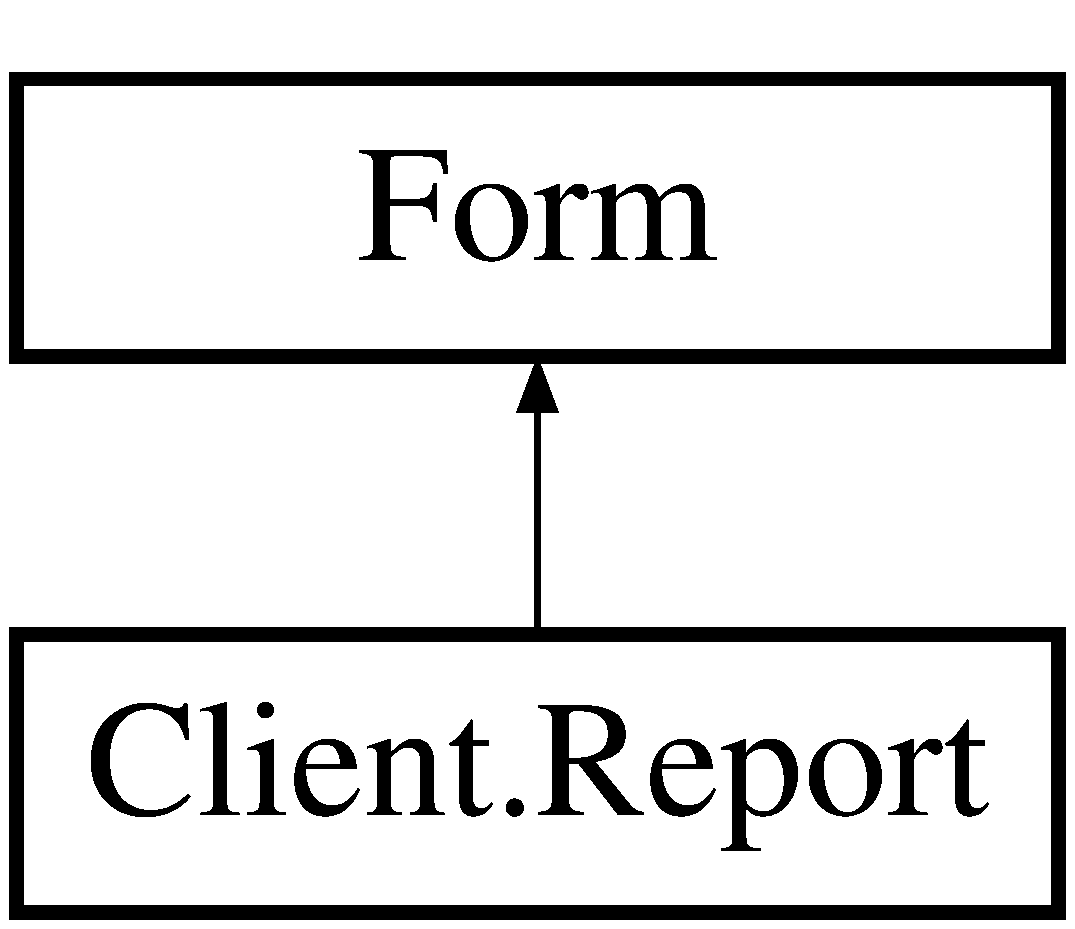
\includegraphics[height=2.000000cm]{class_client_1_1_report}
\end{center}
\end{figure}
\subsection*{Public Member Functions}
\begin{DoxyCompactItemize}
\item 
\hyperlink{class_client_1_1_report_a5982d06a4b2fb26073d40133ebf9deb0}{Report} ()
\begin{DoxyCompactList}\small\item\em Конструктор класс отчет \end{DoxyCompactList}\end{DoxyCompactItemize}
\subsection*{Protected Member Functions}
\begin{DoxyCompactItemize}
\item 
override void \hyperlink{class_client_1_1_report_a83e48fbf05f481d9cbb66f4700131ff6}{Dispose} (bool disposing)
\begin{DoxyCompactList}\small\item\em Clean up any resources being used. \end{DoxyCompactList}\end{DoxyCompactItemize}


\subsection{Detailed Description}
Класс отвечающий за формирование отчета 



\subsection{Constructor \& Destructor Documentation}
\hypertarget{class_client_1_1_report_a5982d06a4b2fb26073d40133ebf9deb0}{}\label{class_client_1_1_report_a5982d06a4b2fb26073d40133ebf9deb0} 
\index{Client\+::\+Report@{Client\+::\+Report}!Report@{Report}}
\index{Report@{Report}!Client\+::\+Report@{Client\+::\+Report}}
\subsubsection{\texorpdfstring{Report()}{Report()}}
{\footnotesize\ttfamily Client.\+Report.\+Report (\begin{DoxyParamCaption}{ }\end{DoxyParamCaption})\hspace{0.3cm}{\ttfamily [inline]}}



Конструктор класс отчет 



\subsection{Member Function Documentation}
\hypertarget{class_client_1_1_report_a83e48fbf05f481d9cbb66f4700131ff6}{}\label{class_client_1_1_report_a83e48fbf05f481d9cbb66f4700131ff6} 
\index{Client\+::\+Report@{Client\+::\+Report}!Dispose@{Dispose}}
\index{Dispose@{Dispose}!Client\+::\+Report@{Client\+::\+Report}}
\subsubsection{\texorpdfstring{Dispose()}{Dispose()}}
{\footnotesize\ttfamily override void Client.\+Report.\+Dispose (\begin{DoxyParamCaption}\item[{bool}]{disposing }\end{DoxyParamCaption})\hspace{0.3cm}{\ttfamily [inline]}, {\ttfamily [protected]}}



Clean up any resources being used. 


\begin{DoxyParams}{Parameters}
{\em disposing} & true if managed resources should be disposed; otherwise, false.\\
\hline
\end{DoxyParams}


The documentation for this class was generated from the following files\+:\begin{DoxyCompactItemize}
\item 
C\+:/\+Users/саша/\+Documents/\+Visual Studio 2015/\+Projects/\+Forex2.\+0/\+Client/Report.\+cs\item 
C\+:/\+Users/саша/\+Documents/\+Visual Studio 2015/\+Projects/\+Forex2.\+0/\+Client/Report.\+Designer.\+cs\end{DoxyCompactItemize}

\hypertarget{class_client_1_1_resistance}{}\section{Client.\+Resistance Class Reference}
\label{class_client_1_1_resistance}\index{Client.\+Resistance@{Client.\+Resistance}}


Класс отвечающий за сущность линии сопротивления  


\subsection*{Public Member Functions}
\begin{DoxyCompactItemize}
\item 
\hyperlink{class_client_1_1_resistance_a8bac71f5502f2fd1f5fa666839bbb4b4}{Resistance} (List$<$ List$<$ double $>$$>$ poin, int tic, double pogr, List$<$ Date\+Time $>$ Date, int h, double M\+A\+XY, double M\+A\+XX, double MaxH, List$<$ double $>$ mass\+Y\+File\+Buy, Chart graphic)
\begin{DoxyCompactList}\small\item\em Формирование линий поддержки \end{DoxyCompactList}\end{DoxyCompactItemize}
\subsection*{Public Attributes}
\begin{DoxyCompactItemize}
\item 
\hypertarget{class_client_1_1_resistance_a7fed455f08370e12fe44a55d6f80cb75}{}\label{class_client_1_1_resistance_a7fed455f08370e12fe44a55d6f80cb75} 
double {\bfseries M\+A\+XY} = 0
\item 
\hypertarget{class_client_1_1_resistance_a041175e708b816692b43162cd423c3f2}{}\label{class_client_1_1_resistance_a041175e708b816692b43162cd423c3f2} 
double {\bfseries M\+A\+XX} = 0
\end{DoxyCompactItemize}


\subsection{Detailed Description}
Класс отвечающий за сущность линии сопротивления 



\subsection{Constructor \& Destructor Documentation}
\hypertarget{class_client_1_1_resistance_a8bac71f5502f2fd1f5fa666839bbb4b4}{}\label{class_client_1_1_resistance_a8bac71f5502f2fd1f5fa666839bbb4b4} 
\index{Client\+::\+Resistance@{Client\+::\+Resistance}!Resistance@{Resistance}}
\index{Resistance@{Resistance}!Client\+::\+Resistance@{Client\+::\+Resistance}}
\subsubsection{\texorpdfstring{Resistance()}{Resistance()}}
{\footnotesize\ttfamily Client.\+Resistance.\+Resistance (\begin{DoxyParamCaption}\item[{List$<$ List$<$ double $>$$>$}]{poin,  }\item[{int}]{tic,  }\item[{double}]{pogr,  }\item[{List$<$ Date\+Time $>$}]{Date,  }\item[{int}]{h,  }\item[{double}]{M\+A\+XY,  }\item[{double}]{M\+A\+XX,  }\item[{double}]{MaxH,  }\item[{List$<$ double $>$}]{mass\+Y\+File\+Buy,  }\item[{Chart}]{graphic }\end{DoxyParamCaption})\hspace{0.3cm}{\ttfamily [inline]}}



Формирование линий поддержки 


\begin{DoxyParams}{Parameters}
{\em poin} & Точки минимумов и максимов\\
\hline
{\em tic} & Прошедшее время с начала запуска\\
\hline
{\em pogr} & Некоторая погрешность в пределах которой формируется линия\\
\hline
{\em h} & ???\\
\hline
{\em M\+I\+NY} & ???\\
\hline
{\em M\+I\+NX} & ???\\
\hline
{\em MinH} & ???\\
\hline
\end{DoxyParams}


The documentation for this class was generated from the following file\+:\begin{DoxyCompactItemize}
\item 
C\+:/\+Users/саша/\+Documents/\+Visual Studio 2015/\+Projects/\+Forex2.\+0/\+Client/Resistance.\+cs\end{DoxyCompactItemize}

\hypertarget{class_client_1_1_setting}{}\section{Client.\+Setting Class Reference}
\label{class_client_1_1_setting}\index{Client.\+Setting@{Client.\+Setting}}


Класс для задания размеров окнаы  


Inheritance diagram for Client.\+Setting\+:\begin{figure}[H]
\begin{center}
\leavevmode
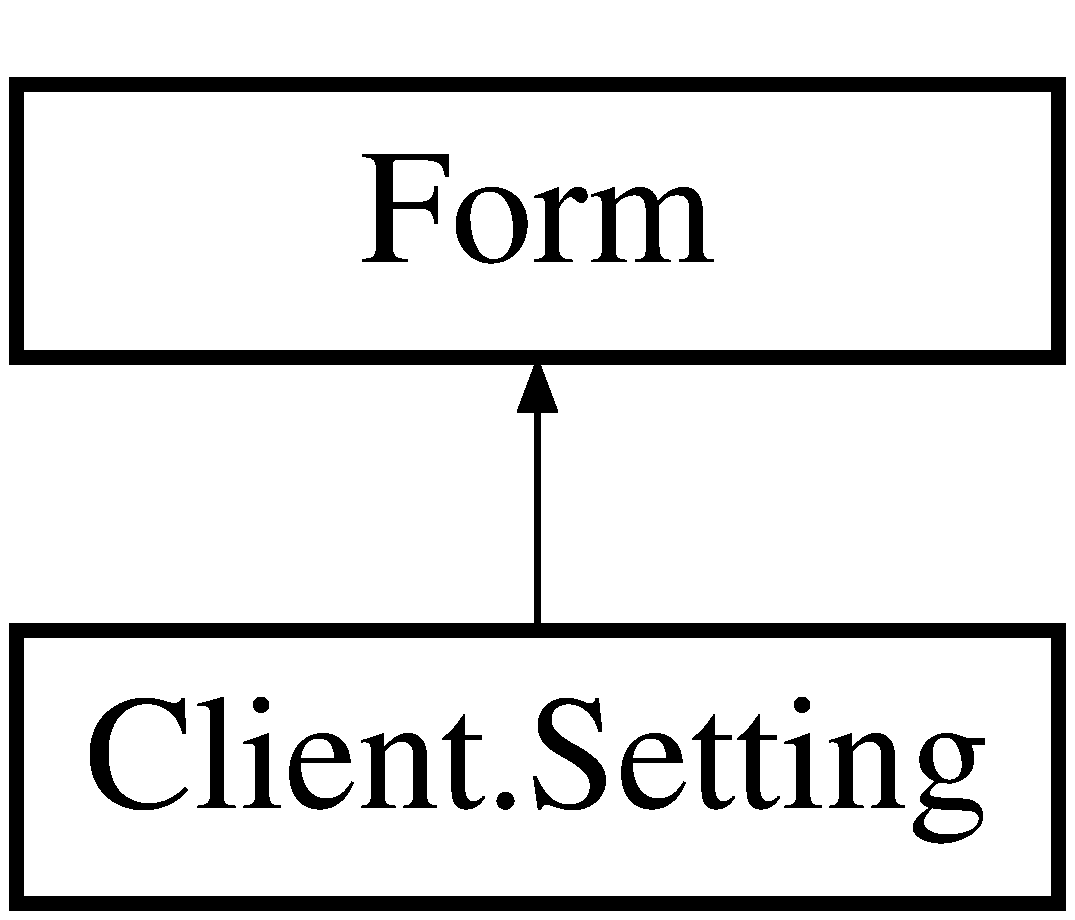
\includegraphics[height=2.000000cm]{class_client_1_1_setting}
\end{center}
\end{figure}
\subsection*{Public Member Functions}
\begin{DoxyCompactItemize}
\item 
\hyperlink{class_client_1_1_setting_a733582576c54cf20fd2437cd1240a97c}{Setting} ()
\begin{DoxyCompactList}\small\item\em Initialize \end{DoxyCompactList}\end{DoxyCompactItemize}
\subsection*{Protected Member Functions}
\begin{DoxyCompactItemize}
\item 
override void \hyperlink{class_client_1_1_setting_abcc5beb1a34b3f8076237e7d4bca5b29}{Dispose} (bool disposing)
\begin{DoxyCompactList}\small\item\em Clean up any resources being used. \end{DoxyCompactList}\end{DoxyCompactItemize}


\subsection{Detailed Description}
Класс для задания размеров окнаы 



\subsection{Constructor \& Destructor Documentation}
\hypertarget{class_client_1_1_setting_a733582576c54cf20fd2437cd1240a97c}{}\label{class_client_1_1_setting_a733582576c54cf20fd2437cd1240a97c} 
\index{Client\+::\+Setting@{Client\+::\+Setting}!Setting@{Setting}}
\index{Setting@{Setting}!Client\+::\+Setting@{Client\+::\+Setting}}
\subsubsection{\texorpdfstring{Setting()}{Setting()}}
{\footnotesize\ttfamily Client.\+Setting.\+Setting (\begin{DoxyParamCaption}{ }\end{DoxyParamCaption})\hspace{0.3cm}{\ttfamily [inline]}}



Initialize 



\subsection{Member Function Documentation}
\hypertarget{class_client_1_1_setting_abcc5beb1a34b3f8076237e7d4bca5b29}{}\label{class_client_1_1_setting_abcc5beb1a34b3f8076237e7d4bca5b29} 
\index{Client\+::\+Setting@{Client\+::\+Setting}!Dispose@{Dispose}}
\index{Dispose@{Dispose}!Client\+::\+Setting@{Client\+::\+Setting}}
\subsubsection{\texorpdfstring{Dispose()}{Dispose()}}
{\footnotesize\ttfamily override void Client.\+Setting.\+Dispose (\begin{DoxyParamCaption}\item[{bool}]{disposing }\end{DoxyParamCaption})\hspace{0.3cm}{\ttfamily [inline]}, {\ttfamily [protected]}}



Clean up any resources being used. 


\begin{DoxyParams}{Parameters}
{\em disposing} & true if managed resources should be disposed; otherwise, false.\\
\hline
\end{DoxyParams}


The documentation for this class was generated from the following files\+:\begin{DoxyCompactItemize}
\item 
C\+:/\+Users/саша/\+Documents/\+Visual Studio 2015/\+Projects/\+Forex2.\+0/\+Client/Setting.\+cs\item 
C\+:/\+Users/саша/\+Documents/\+Visual Studio 2015/\+Projects/\+Forex2.\+0/\+Client/Setting.\+Designer.\+cs\end{DoxyCompactItemize}

\hypertarget{class_client_1_1_splice}{}\section{Client.\+Splice Class Reference}
\label{class_client_1_1_splice}\index{Client.\+Splice@{Client.\+Splice}}


Класс соединяющий буферные значения с файловыми  


\subsection*{Public Member Functions}
\begin{DoxyCompactItemize}
\item 
List$<$ double $>$ \hyperlink{class_client_1_1_splice_a49f90f5d0d645303e1c467300148a02e}{glue} (List$<$ double $>$ File, List$<$ double $>$ Buffer, int tic, int Chislo\+Zagruz)
\begin{DoxyCompactList}\small\item\em Метод склейки буферных данных и файловых + \end{DoxyCompactList}\item 
List$<$ double $>$ \hyperlink{class_client_1_1_splice_a40730137c3ada57dc527824383102584}{glue} (List$<$ double $>$ Buffer, List$<$ double $>$ File)
\begin{DoxyCompactList}\small\item\em Метод склейки и последнего числа буфера и файла + \end{DoxyCompactList}\item 
List$<$ Date\+Time $>$ \hyperlink{class_client_1_1_splice_a061e8b37cd63aef0dbbe951019f7af4f}{glue} (List$<$ Date\+Time $>$ Ftime, List$<$ Date\+Time $>$ I\+Time, int tic, int Chislo\+Zagruz)
\begin{DoxyCompactList}\small\item\em Метод склейки буферного времени и файлового + \end{DoxyCompactList}\item 
List$<$ Date\+Time $>$ \hyperlink{class_client_1_1_splice_adf5f1bc6d5a0060eb8169337217a0a99}{glue} (List$<$ Date\+Time $>$ Ftime, List$<$ Date\+Time $>$ I\+Time)
\begin{DoxyCompactList}\small\item\em Метод склейки и последнего числа буфера и файла + \end{DoxyCompactList}\end{DoxyCompactItemize}


\subsection{Detailed Description}
Класс соединяющий буферные значения с файловыми 



\subsection{Member Function Documentation}
\hypertarget{class_client_1_1_splice_a49f90f5d0d645303e1c467300148a02e}{}\label{class_client_1_1_splice_a49f90f5d0d645303e1c467300148a02e} 
\index{Client\+::\+Splice@{Client\+::\+Splice}!glue@{glue}}
\index{glue@{glue}!Client\+::\+Splice@{Client\+::\+Splice}}
\subsubsection{\texorpdfstring{glue()}{glue()}\hspace{0.1cm}{\footnotesize\ttfamily [1/4]}}
{\footnotesize\ttfamily List$<$double$>$ Client.\+Splice.\+glue (\begin{DoxyParamCaption}\item[{List$<$ double $>$}]{File,  }\item[{List$<$ double $>$}]{Buffer,  }\item[{int}]{tic,  }\item[{int}]{Chislo\+Zagruz }\end{DoxyParamCaption})\hspace{0.3cm}{\ttfamily [inline]}}



Метод склейки буферных данных и файловых + 


\begin{DoxyParams}{Parameters}
{\em Buffer} & double значения 1 листа.\\
\hline
{\em File} & double значения 2 листа.\\
\hline
{\em tic} & int время которое прошло с запуска формы.\\
\hline
{\em Chislo\+Zagruz} & число загрузок из файла.\\
\hline
\end{DoxyParams}
\begin{DoxyReturn}{Returns}
Объединенный лист
\end{DoxyReturn}
\hypertarget{class_client_1_1_splice_a40730137c3ada57dc527824383102584}{}\label{class_client_1_1_splice_a40730137c3ada57dc527824383102584} 
\index{Client\+::\+Splice@{Client\+::\+Splice}!glue@{glue}}
\index{glue@{glue}!Client\+::\+Splice@{Client\+::\+Splice}}
\subsubsection{\texorpdfstring{glue()}{glue()}\hspace{0.1cm}{\footnotesize\ttfamily [2/4]}}
{\footnotesize\ttfamily List$<$double$>$ Client.\+Splice.\+glue (\begin{DoxyParamCaption}\item[{List$<$ double $>$}]{Buffer,  }\item[{List$<$ double $>$}]{File }\end{DoxyParamCaption})\hspace{0.3cm}{\ttfamily [inline]}}



Метод склейки и последнего числа буфера и файла + 


\begin{DoxyParams}{Parameters}
{\em Buffer} & double значения 1 листа.\\
\hline
{\em File} & double значения 2 листа.\\
\hline
\end{DoxyParams}
\begin{DoxyReturn}{Returns}
Объединенный лист
\end{DoxyReturn}
\hypertarget{class_client_1_1_splice_a061e8b37cd63aef0dbbe951019f7af4f}{}\label{class_client_1_1_splice_a061e8b37cd63aef0dbbe951019f7af4f} 
\index{Client\+::\+Splice@{Client\+::\+Splice}!glue@{glue}}
\index{glue@{glue}!Client\+::\+Splice@{Client\+::\+Splice}}
\subsubsection{\texorpdfstring{glue()}{glue()}\hspace{0.1cm}{\footnotesize\ttfamily [3/4]}}
{\footnotesize\ttfamily List$<$Date\+Time$>$ Client.\+Splice.\+glue (\begin{DoxyParamCaption}\item[{List$<$ Date\+Time $>$}]{Ftime,  }\item[{List$<$ Date\+Time $>$}]{I\+Time,  }\item[{int}]{tic,  }\item[{int}]{Chislo\+Zagruz }\end{DoxyParamCaption})\hspace{0.3cm}{\ttfamily [inline]}}



Метод склейки буферного времени и файлового + 


\begin{DoxyParams}{Parameters}
{\em Ftime} & Date\+Time значения 1 листа файловых.\\
\hline
{\em I\+Time} & Date\+Time значения 2 листа буферных.\\
\hline
{\em tic} & int время которое прошло с запуска формы.\\
\hline
{\em Chislo\+Zagruz} & число загрузок из файла.\\
\hline
\end{DoxyParams}
\begin{DoxyReturn}{Returns}
Объединенный лист
\end{DoxyReturn}
\hypertarget{class_client_1_1_splice_adf5f1bc6d5a0060eb8169337217a0a99}{}\label{class_client_1_1_splice_adf5f1bc6d5a0060eb8169337217a0a99} 
\index{Client\+::\+Splice@{Client\+::\+Splice}!glue@{glue}}
\index{glue@{glue}!Client\+::\+Splice@{Client\+::\+Splice}}
\subsubsection{\texorpdfstring{glue()}{glue()}\hspace{0.1cm}{\footnotesize\ttfamily [4/4]}}
{\footnotesize\ttfamily List$<$Date\+Time$>$ Client.\+Splice.\+glue (\begin{DoxyParamCaption}\item[{List$<$ Date\+Time $>$}]{Ftime,  }\item[{List$<$ Date\+Time $>$}]{I\+Time }\end{DoxyParamCaption})\hspace{0.3cm}{\ttfamily [inline]}}



Метод склейки и последнего числа буфера и файла + 


\begin{DoxyParams}{Parameters}
{\em Buffer} & double значения 1 листа.\\
\hline
{\em File} & double значения 2 листа.\\
\hline
\end{DoxyParams}
\begin{DoxyReturn}{Returns}
Объединенный лист
\end{DoxyReturn}


The documentation for this class was generated from the following file\+:\begin{DoxyCompactItemize}
\item 
C\+:/\+Users/саша/\+Documents/\+Visual Studio 2015/\+Projects/\+Forex2.\+0/\+Client/Splice.\+cs\end{DoxyCompactItemize}

\hypertarget{class_client_1_1_support}{}\section{Client.\+Support Class Reference}
\label{class_client_1_1_support}\index{Client.\+Support@{Client.\+Support}}


класс отвечает за создание сущности линии поддержки  


\subsection*{Public Member Functions}
\begin{DoxyCompactItemize}
\item 
\hyperlink{class_client_1_1_support_a804e4ee7bda6034926efbb589a81b25c}{Support} (List$<$ List$<$ double $>$$>$ poin, int tic, double pogr, List$<$ Date\+Time $>$ Date, int h, double M\+I\+NY, double M\+I\+NX, double MinH, List$<$ double $>$ mass\+Y\+File\+Buy, Chart graphic)
\begin{DoxyCompactList}\small\item\em Формирование линий поддержки \end{DoxyCompactList}\end{DoxyCompactItemize}
\subsection*{Public Attributes}
\begin{DoxyCompactItemize}
\item 
\hypertarget{class_client_1_1_support_a017d64dcbcac36472cabcd36294966c2}{}\label{class_client_1_1_support_a017d64dcbcac36472cabcd36294966c2} 
double {\bfseries M\+I\+NY} = 0
\item 
\hypertarget{class_client_1_1_support_a59fef07f9629cd08e8b359390465c342}{}\label{class_client_1_1_support_a59fef07f9629cd08e8b359390465c342} 
double {\bfseries M\+I\+NX} = 0
\end{DoxyCompactItemize}


\subsection{Detailed Description}
класс отвечает за создание сущности линии поддержки 



\subsection{Constructor \& Destructor Documentation}
\hypertarget{class_client_1_1_support_a804e4ee7bda6034926efbb589a81b25c}{}\label{class_client_1_1_support_a804e4ee7bda6034926efbb589a81b25c} 
\index{Client\+::\+Support@{Client\+::\+Support}!Support@{Support}}
\index{Support@{Support}!Client\+::\+Support@{Client\+::\+Support}}
\subsubsection{\texorpdfstring{Support()}{Support()}}
{\footnotesize\ttfamily Client.\+Support.\+Support (\begin{DoxyParamCaption}\item[{List$<$ List$<$ double $>$$>$}]{poin,  }\item[{int}]{tic,  }\item[{double}]{pogr,  }\item[{List$<$ Date\+Time $>$}]{Date,  }\item[{int}]{h,  }\item[{double}]{M\+I\+NY,  }\item[{double}]{M\+I\+NX,  }\item[{double}]{MinH,  }\item[{List$<$ double $>$}]{mass\+Y\+File\+Buy,  }\item[{Chart}]{graphic }\end{DoxyParamCaption})\hspace{0.3cm}{\ttfamily [inline]}}



Формирование линий поддержки 


\begin{DoxyParams}{Parameters}
{\em poin} & Точки минимумов и максимов\\
\hline
{\em tic} & Прошедшее время с начала запуска\\
\hline
{\em pogr} & Некоторая погрешность в пределах которой формируется линия\\
\hline
{\em h} & ???\\
\hline
{\em M\+I\+NY} & ???\\
\hline
{\em M\+I\+NX} & ???\\
\hline
{\em MinH} & ???\\
\hline
\end{DoxyParams}


The documentation for this class was generated from the following file\+:\begin{DoxyCompactItemize}
\item 
C\+:/\+Users/саша/\+Documents/\+Visual Studio 2015/\+Projects/\+Forex2.\+0/\+Client/Support.\+cs\end{DoxyCompactItemize}

\hypertarget{class_client_1_1_s_window}{}\section{Client.\+S\+Window Class Reference}
\label{class_client_1_1_s_window}\index{Client.\+S\+Window@{Client.\+S\+Window}}


класс для задание размеров формы котировки  


Inheritance diagram for Client.\+S\+Window\+:\begin{figure}[H]
\begin{center}
\leavevmode
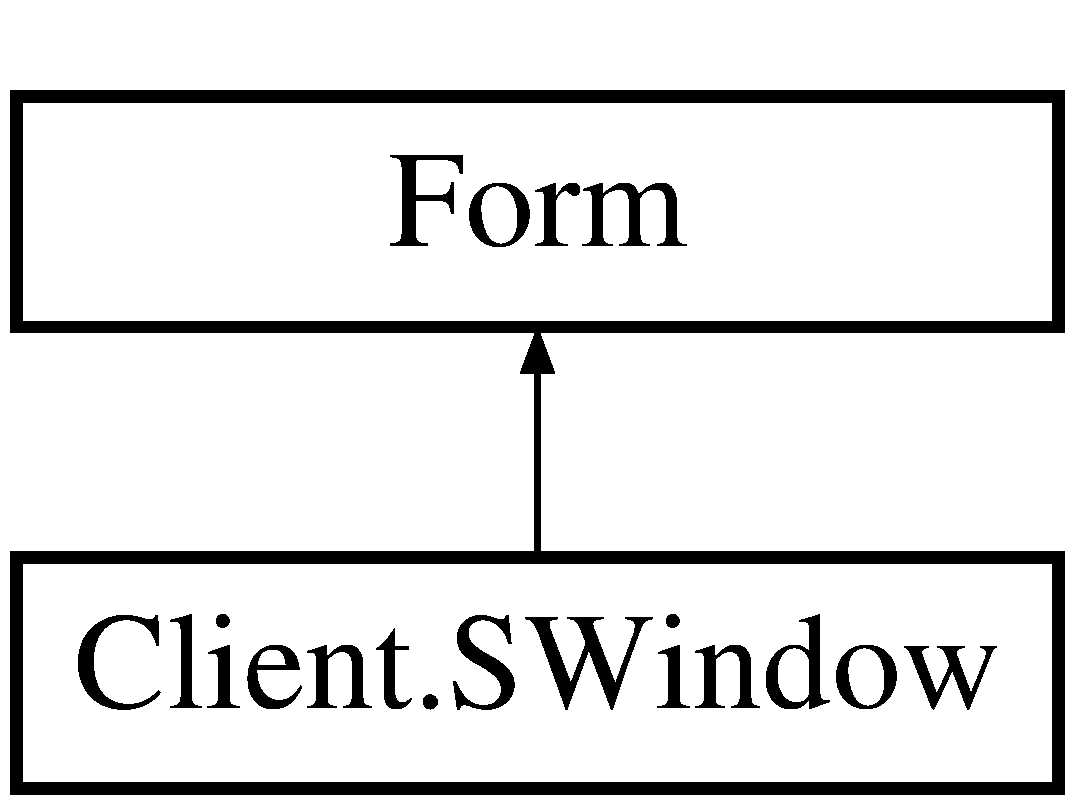
\includegraphics[height=2.000000cm]{class_client_1_1_s_window}
\end{center}
\end{figure}
\subsection*{Public Member Functions}
\begin{DoxyCompactItemize}
\item 
\hyperlink{class_client_1_1_s_window_a7688faaaf1b0ea097066142fc9d90326}{S\+Window} ()
\begin{DoxyCompactList}\small\item\em Main \end{DoxyCompactList}\end{DoxyCompactItemize}
\subsection*{Protected Member Functions}
\begin{DoxyCompactItemize}
\item 
override void \hyperlink{class_client_1_1_s_window_a06a09e3c69c7ed01bf7a96ebbc90c12b}{Dispose} (bool disposing)
\begin{DoxyCompactList}\small\item\em Clean up any resources being used. \end{DoxyCompactList}\end{DoxyCompactItemize}


\subsection{Detailed Description}
класс для задание размеров формы котировки 



\subsection{Constructor \& Destructor Documentation}
\hypertarget{class_client_1_1_s_window_a7688faaaf1b0ea097066142fc9d90326}{}\label{class_client_1_1_s_window_a7688faaaf1b0ea097066142fc9d90326} 
\index{Client\+::\+S\+Window@{Client\+::\+S\+Window}!S\+Window@{S\+Window}}
\index{S\+Window@{S\+Window}!Client\+::\+S\+Window@{Client\+::\+S\+Window}}
\subsubsection{\texorpdfstring{S\+Window()}{SWindow()}}
{\footnotesize\ttfamily Client.\+S\+Window.\+S\+Window (\begin{DoxyParamCaption}{ }\end{DoxyParamCaption})\hspace{0.3cm}{\ttfamily [inline]}}



Main 



\subsection{Member Function Documentation}
\hypertarget{class_client_1_1_s_window_a06a09e3c69c7ed01bf7a96ebbc90c12b}{}\label{class_client_1_1_s_window_a06a09e3c69c7ed01bf7a96ebbc90c12b} 
\index{Client\+::\+S\+Window@{Client\+::\+S\+Window}!Dispose@{Dispose}}
\index{Dispose@{Dispose}!Client\+::\+S\+Window@{Client\+::\+S\+Window}}
\subsubsection{\texorpdfstring{Dispose()}{Dispose()}}
{\footnotesize\ttfamily override void Client.\+S\+Window.\+Dispose (\begin{DoxyParamCaption}\item[{bool}]{disposing }\end{DoxyParamCaption})\hspace{0.3cm}{\ttfamily [inline]}, {\ttfamily [protected]}}



Clean up any resources being used. 


\begin{DoxyParams}{Parameters}
{\em disposing} & true if managed resources should be disposed; otherwise, false.\\
\hline
\end{DoxyParams}


The documentation for this class was generated from the following files\+:\begin{DoxyCompactItemize}
\item 
C\+:/\+Users/саша/\+Documents/\+Visual Studio 2015/\+Projects/\+Forex2.\+0/\+Client/S\+Window.\+cs\item 
C\+:/\+Users/саша/\+Documents/\+Visual Studio 2015/\+Projects/\+Forex2.\+0/\+Client/S\+Window.\+Designer.\+cs\end{DoxyCompactItemize}

\hypertarget{class_client_1_1_windowd}{}\section{Client.\+Windowd Class Reference}
\label{class_client_1_1_windowd}\index{Client.\+Windowd@{Client.\+Windowd}}


Форма для взаиможействия с графиками котировок и создания сделок  


Inheritance diagram for Client.\+Windowd\+:\begin{figure}[H]
\begin{center}
\leavevmode
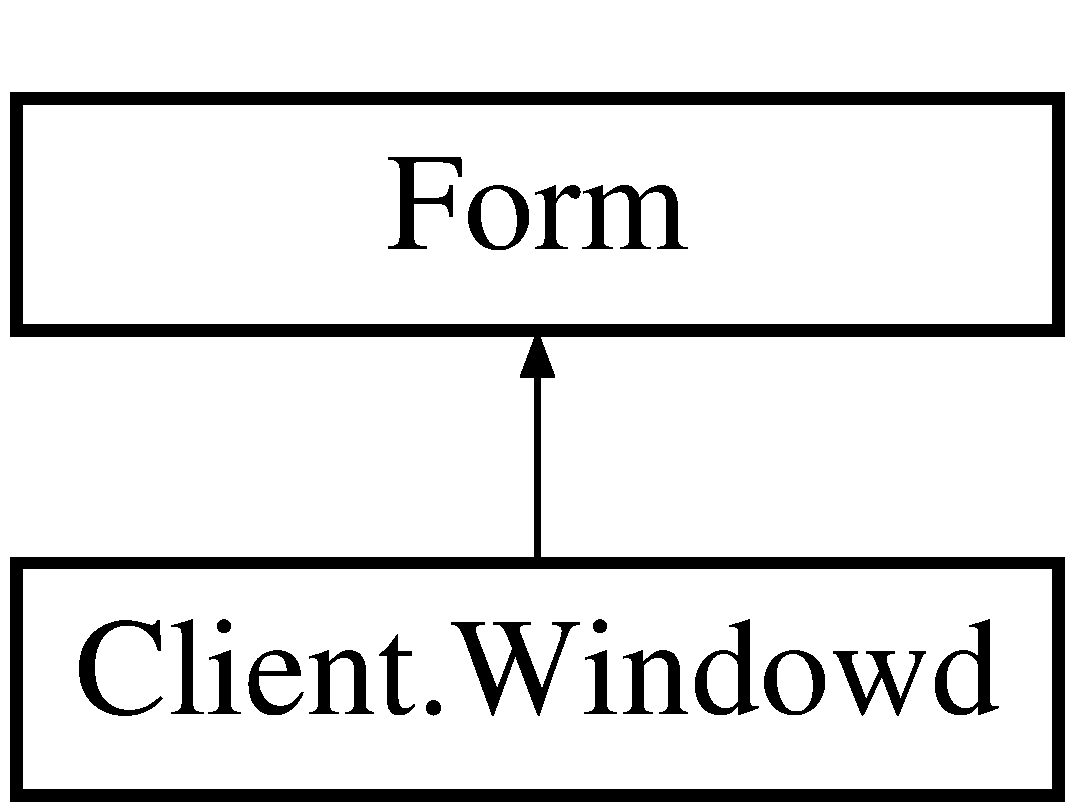
\includegraphics[height=2.000000cm]{class_client_1_1_windowd}
\end{center}
\end{figure}
\subsection*{Public Member Functions}
\begin{DoxyCompactItemize}
\item 
\hyperlink{class_client_1_1_windowd_a8eaca5bbdf54bb33864c1b433ccb63cd}{Windowd} (string Vvalue)
\begin{DoxyCompactList}\small\item\em Cоздание окна валюты \end{DoxyCompactList}\item 
void \hyperlink{class_client_1_1_windowd_a318f722574a5396b688223fcec6e080c}{Activ} (object sender)
\begin{DoxyCompactList}\small\item\em Method create file \end{DoxyCompactList}\item 
void \hyperlink{class_client_1_1_windowd_aa308a6bcf8931b033272affc8076e96a}{t\+Tip} ()
\begin{DoxyCompactList}\small\item\em Метод перевода тултипов \end{DoxyCompactList}\item 
void \hyperlink{class_client_1_1_windowd_a081f7fdb62ef1cefe2ce4dacc45eb41b}{Button} ()
\begin{DoxyCompactList}\small\item\em Метод перевода кнопок \end{DoxyCompactList}\item 
void \hyperlink{class_client_1_1_windowd_a3b7eabc5c91768d6442af8fc585edb87}{Menu} ()
\begin{DoxyCompactList}\small\item\em Метод перевода меню \end{DoxyCompactList}\item 
int \hyperlink{class_client_1_1_windowd_ab924a9e1fb51713d4e42a0dc60301625}{Update} (int \hyperlink{class_client_1_1_windowd_af0c658d1138b70eeafdbc105ec2d7a81}{tic}, List$<$ Date\+Time $>$ DateT, double Now\+Time, List$<$ Date\+Time $>$ \hyperlink{class_client_1_1_windowd_a98b5779ed4abf0571a16deb0c985a7a4}{D\+I\+N\+ET})
\begin{DoxyCompactList}\small\item\em Метод задания параметров линии и обновления данных \end{DoxyCompactList}\item 
void \hyperlink{class_client_1_1_windowd_aac30e6623a96e0bc508e9f4e82d4bb65}{ZoomT} (int zoom\+Chart, int \hyperlink{class_client_1_1_windowd_af0c658d1138b70eeafdbc105ec2d7a81}{tic})
\begin{DoxyCompactList}\small\item\em Изменение маштаба \end{DoxyCompactList}\item 
void \hyperlink{class_client_1_1_windowd_ad43dbe14134a90f8cd6acf4da36e485c}{Draw\+S\+MA} (List$<$ Date\+Time $>$ Dat, int Sglag, List$<$ double $>$ Buff, List$<$ double $>$ sreds)
\begin{DoxyCompactList}\small\item\em Строит линию на графике \end{DoxyCompactList}\item 
void \hyperlink{class_client_1_1_windowd_a84177c165ee297b49e25c6b5da053c12}{Draw\+Min\+Max} (List$<$ List$<$ double $>$$>$ poin)
\begin{DoxyCompactList}\small\item\em Построение линий минимумов и максимумов \end{DoxyCompactList}\item 
void \hyperlink{class_client_1_1_windowd_a7c775dee3ca111b2a04d2821b3daf35f}{ini\+Line\+Min\+Max} (Chart graphic, int index)
\begin{DoxyCompactList}\small\item\em Задание цвета линии \end{DoxyCompactList}\item 
void \hyperlink{class_client_1_1_windowd_ae28446da17026602dc8e9146af4c542d}{Resis} (List$<$ List$<$ double $>$$>$ poin, int \hyperlink{class_client_1_1_windowd_af0c658d1138b70eeafdbc105ec2d7a81}{tic}, double pogr, List$<$ Date\+Time $>$ Date)
\begin{DoxyCompactList}\small\item\em Формирование линий сопротивлений \end{DoxyCompactList}\item 
void \hyperlink{class_client_1_1_windowd_a8b8c230d223b1ba05dd936ff7cbc6e60}{prisvoenie} (int h, double Y, List$<$ List$<$ double $>$$>$ poin, double X, double Mh)
\begin{DoxyCompactList}\small\item\em Получение точек путем сравнивания предыдущих точек \end{DoxyCompactList}\item 
void \hyperlink{class_client_1_1_windowd_a8e1e4f8f41d93b2961b1a4733c1c2ebc}{Window\+\_\+\+Load} (object sender, Event\+Args e)
\item 
double \hyperlink{class_client_1_1_windowd_acf6504da17d839fd206b3fe0710db4ec}{Second\+Conect} ()
\begin{DoxyCompactList}\small\item\em Метод посекундного конекта \end{DoxyCompactList}\end{DoxyCompactItemize}
\subsection*{Public Attributes}
\begin{DoxyCompactItemize}
\item 
Chart\+Area \hyperlink{class_client_1_1_windowd_aed40d5c999bd377a5e6a11b6f09e3f9c}{area} = new Chart\+Area()
\begin{DoxyCompactList}\small\item\em область \end{DoxyCompactList}\item 
int \hyperlink{class_client_1_1_windowd_aa41017ef66a809df6898262c5a425303}{Zoom} = 100
\begin{DoxyCompactList}\small\item\em Количетво рассматривомого времени в Unixtime \end{DoxyCompactList}\item 
int \hyperlink{class_client_1_1_windowd_a960143b9372a3a7dc576b4578aa40bd8}{danoe} = 0
\begin{DoxyCompactList}\small\item\em Количетво рассматривомого времени в Unixtime \end{DoxyCompactList}\item 
string \hyperlink{class_client_1_1_windowd_a7d221cc5d9347a6064b09db206894342}{value}
\begin{DoxyCompactList}\small\item\em Содержит наименование валюты \end{DoxyCompactList}\item 
double \hyperlink{class_client_1_1_windowd_a0f5b6aebf0f3c23cd708480bfc87d1bb}{poslchislo\+Sell}
\begin{DoxyCompactList}\small\item\em Последнее число продажи \end{DoxyCompactList}\item 
double \hyperlink{class_client_1_1_windowd_a18e884676837904afa8857d7abd6fc7b}{poslchislo\+Buy}
\begin{DoxyCompactList}\small\item\em Последнее число покупкки \end{DoxyCompactList}\item 
bool \hyperlink{class_client_1_1_windowd_a89f97a16687dad532281e065e70bd490}{inet}
\begin{DoxyCompactList}\small\item\em Поле хранящее конект \end{DoxyCompactList}\item 
List$<$ \hyperlink{class_client_1_1_deal}{Deal} $>$ \hyperlink{class_client_1_1_windowd_aec1343722b0bde8b263e8258fc8f806c}{B\+UY} = new List$<$\hyperlink{class_client_1_1_deal}{Deal}$>$()
\begin{DoxyCompactList}\small\item\em Поле хранящее конект \end{DoxyCompactList}\item 
List$<$ \hyperlink{class_client_1_1_deal}{Deal} $>$ \hyperlink{class_client_1_1_windowd_a1616dcfb8b780f2ff45f74a76cb7d997}{S\+E\+LL} = new List$<$\hyperlink{class_client_1_1_deal}{Deal}$>$()
\begin{DoxyCompactList}\small\item\em лист объектов хранящий продажи \end{DoxyCompactList}\item 
List$<$ double $>$ \hyperlink{class_client_1_1_windowd_a63515d43501540d22908b3e75b0446e6}{BufferB} = new List$<$double$>$()
\begin{DoxyCompactList}\small\item\em Буфферное значение покупки \end{DoxyCompactList}\item 
List$<$ double $>$ \hyperlink{class_client_1_1_windowd_a923a51f80de2de0db93114454f23e6cb}{BufferS} = new List$<$double$>$()
\begin{DoxyCompactList}\small\item\em Буфферное значение продажи \end{DoxyCompactList}\item 
List$<$ Date\+Time $>$ \hyperlink{class_client_1_1_windowd_ae56192c0587527c76b5878d3239768e4}{D\+B\+UF} = new List$<$Date\+Time$>$()
\begin{DoxyCompactList}\small\item\em Буфферное значение времени \end{DoxyCompactList}\item 
List$<$ Date\+Time $>$ \hyperlink{class_client_1_1_windowd_a98b5779ed4abf0571a16deb0c985a7a4}{D\+I\+N\+ET} = new List$<$Date\+Time$>$()
\begin{DoxyCompactList}\small\item\em значение времени с интернета \end{DoxyCompactList}\item 
int \hyperlink{class_client_1_1_windowd_af0c658d1138b70eeafdbc105ec2d7a81}{tic} = 0
\begin{DoxyCompactList}\small\item\em Поле отслеживающие кол-\/во прошедших секунд с запуска формы \end{DoxyCompactList}\end{DoxyCompactItemize}
\subsection*{Protected Member Functions}
\begin{DoxyCompactItemize}
\item 
override void \hyperlink{class_client_1_1_windowd_ae3b81759148b68ad5f55e959567b5aab}{Dispose} (bool disposing)
\begin{DoxyCompactList}\small\item\em Clean up any resources being used. \end{DoxyCompactList}\end{DoxyCompactItemize}


\subsection{Detailed Description}
Форма для взаиможействия с графиками котировок и создания сделок 


\begin{DoxyParams}{Parameters}
{\em quotations} & объект сделка\\
\hline
{\em bufferS} & Массив покупки\\
\hline
{\em tic} & текущее время отначала торгов\\
\hline
\end{DoxyParams}


\subsection{Constructor \& Destructor Documentation}
\hypertarget{class_client_1_1_windowd_a8eaca5bbdf54bb33864c1b433ccb63cd}{}\label{class_client_1_1_windowd_a8eaca5bbdf54bb33864c1b433ccb63cd} 
\index{Client\+::\+Windowd@{Client\+::\+Windowd}!Windowd@{Windowd}}
\index{Windowd@{Windowd}!Client\+::\+Windowd@{Client\+::\+Windowd}}
\subsubsection{\texorpdfstring{Windowd()}{Windowd()}}
{\footnotesize\ttfamily Client.\+Windowd.\+Windowd (\begin{DoxyParamCaption}\item[{string}]{Vvalue }\end{DoxyParamCaption})\hspace{0.3cm}{\ttfamily [inline]}}



Cоздание окна валюты 


\begin{DoxyParams}{Parameters}
{\em  Vvalue} & Наименование валюты\\
\hline
\end{DoxyParams}


\subsection{Member Function Documentation}
\hypertarget{class_client_1_1_windowd_a318f722574a5396b688223fcec6e080c}{}\label{class_client_1_1_windowd_a318f722574a5396b688223fcec6e080c} 
\index{Client\+::\+Windowd@{Client\+::\+Windowd}!Activ@{Activ}}
\index{Activ@{Activ}!Client\+::\+Windowd@{Client\+::\+Windowd}}
\subsubsection{\texorpdfstring{Activ()}{Activ()}}
{\footnotesize\ttfamily void Client.\+Windowd.\+Activ (\begin{DoxyParamCaption}\item[{object}]{sender }\end{DoxyParamCaption})\hspace{0.3cm}{\ttfamily [inline]}}



Method create file 

\hypertarget{class_client_1_1_windowd_a081f7fdb62ef1cefe2ce4dacc45eb41b}{}\label{class_client_1_1_windowd_a081f7fdb62ef1cefe2ce4dacc45eb41b} 
\index{Client\+::\+Windowd@{Client\+::\+Windowd}!Button@{Button}}
\index{Button@{Button}!Client\+::\+Windowd@{Client\+::\+Windowd}}
\subsubsection{\texorpdfstring{Button()}{Button()}}
{\footnotesize\ttfamily void Client.\+Windowd.\+Button (\begin{DoxyParamCaption}{ }\end{DoxyParamCaption})\hspace{0.3cm}{\ttfamily [inline]}}



Метод перевода кнопок 

\hypertarget{class_client_1_1_windowd_ae3b81759148b68ad5f55e959567b5aab}{}\label{class_client_1_1_windowd_ae3b81759148b68ad5f55e959567b5aab} 
\index{Client\+::\+Windowd@{Client\+::\+Windowd}!Dispose@{Dispose}}
\index{Dispose@{Dispose}!Client\+::\+Windowd@{Client\+::\+Windowd}}
\subsubsection{\texorpdfstring{Dispose()}{Dispose()}}
{\footnotesize\ttfamily override void Client.\+Windowd.\+Dispose (\begin{DoxyParamCaption}\item[{bool}]{disposing }\end{DoxyParamCaption})\hspace{0.3cm}{\ttfamily [inline]}, {\ttfamily [protected]}}



Clean up any resources being used. 


\begin{DoxyParams}{Parameters}
{\em disposing} & true if managed resources should be disposed; otherwise, false.\\
\hline
\end{DoxyParams}
\hypertarget{class_client_1_1_windowd_a84177c165ee297b49e25c6b5da053c12}{}\label{class_client_1_1_windowd_a84177c165ee297b49e25c6b5da053c12} 
\index{Client\+::\+Windowd@{Client\+::\+Windowd}!Draw\+Min\+Max@{Draw\+Min\+Max}}
\index{Draw\+Min\+Max@{Draw\+Min\+Max}!Client\+::\+Windowd@{Client\+::\+Windowd}}
\subsubsection{\texorpdfstring{Draw\+Min\+Max()}{DrawMinMax()}}
{\footnotesize\ttfamily void Client.\+Windowd.\+Draw\+Min\+Max (\begin{DoxyParamCaption}\item[{List$<$ List$<$ double $>$$>$}]{poin }\end{DoxyParamCaption})\hspace{0.3cm}{\ttfamily [inline]}}



Построение линий минимумов и максимумов 


\begin{DoxyParams}{Parameters}
{\em poin} & Точки минимумов и максимов\\
\hline
\end{DoxyParams}
\hypertarget{class_client_1_1_windowd_ad43dbe14134a90f8cd6acf4da36e485c}{}\label{class_client_1_1_windowd_ad43dbe14134a90f8cd6acf4da36e485c} 
\index{Client\+::\+Windowd@{Client\+::\+Windowd}!Draw\+S\+MA@{Draw\+S\+MA}}
\index{Draw\+S\+MA@{Draw\+S\+MA}!Client\+::\+Windowd@{Client\+::\+Windowd}}
\subsubsection{\texorpdfstring{Draw\+S\+M\+A()}{DrawSMA()}}
{\footnotesize\ttfamily void Client.\+Windowd.\+Draw\+S\+MA (\begin{DoxyParamCaption}\item[{List$<$ Date\+Time $>$}]{Dat,  }\item[{int}]{Sglag,  }\item[{List$<$ double $>$}]{Buff,  }\item[{List$<$ double $>$}]{sreds }\end{DoxyParamCaption})\hspace{0.3cm}{\ttfamily [inline]}}



Строит линию на графике 


\begin{DoxyParams}{Parameters}
{\em Dat} & время прошедшее с запуска\\
\hline
{\em Sglag} & Текущее приближени\\
\hline
{\em Buff} & Текущее приближени\\
\hline
{\em sreds} & Текущее приближени\\
\hline
\end{DoxyParams}
\hypertarget{class_client_1_1_windowd_a7c775dee3ca111b2a04d2821b3daf35f}{}\label{class_client_1_1_windowd_a7c775dee3ca111b2a04d2821b3daf35f} 
\index{Client\+::\+Windowd@{Client\+::\+Windowd}!ini\+Line\+Min\+Max@{ini\+Line\+Min\+Max}}
\index{ini\+Line\+Min\+Max@{ini\+Line\+Min\+Max}!Client\+::\+Windowd@{Client\+::\+Windowd}}
\subsubsection{\texorpdfstring{ini\+Line\+Min\+Max()}{iniLineMinMax()}}
{\footnotesize\ttfamily void Client.\+Windowd.\+ini\+Line\+Min\+Max (\begin{DoxyParamCaption}\item[{Chart}]{graphic,  }\item[{int}]{index }\end{DoxyParamCaption})\hspace{0.3cm}{\ttfamily [inline]}}



Задание цвета линии 


\begin{DoxyParams}{Parameters}
{\em graphic} & Точки минимумов и максимов\\
\hline
{\em index} & Прошедшее время с начала запуска\\
\hline
\end{DoxyParams}
\hypertarget{class_client_1_1_windowd_a3b7eabc5c91768d6442af8fc585edb87}{}\label{class_client_1_1_windowd_a3b7eabc5c91768d6442af8fc585edb87} 
\index{Client\+::\+Windowd@{Client\+::\+Windowd}!Menu@{Menu}}
\index{Menu@{Menu}!Client\+::\+Windowd@{Client\+::\+Windowd}}
\subsubsection{\texorpdfstring{Menu()}{Menu()}}
{\footnotesize\ttfamily void Client.\+Windowd.\+Menu (\begin{DoxyParamCaption}{ }\end{DoxyParamCaption})\hspace{0.3cm}{\ttfamily [inline]}}



Метод перевода меню 

\hypertarget{class_client_1_1_windowd_a8b8c230d223b1ba05dd936ff7cbc6e60}{}\label{class_client_1_1_windowd_a8b8c230d223b1ba05dd936ff7cbc6e60} 
\index{Client\+::\+Windowd@{Client\+::\+Windowd}!prisvoenie@{prisvoenie}}
\index{prisvoenie@{prisvoenie}!Client\+::\+Windowd@{Client\+::\+Windowd}}
\subsubsection{\texorpdfstring{prisvoenie()}{prisvoenie()}}
{\footnotesize\ttfamily void Client.\+Windowd.\+prisvoenie (\begin{DoxyParamCaption}\item[{int}]{h,  }\item[{double}]{Y,  }\item[{List$<$ List$<$ double $>$$>$}]{poin,  }\item[{double}]{X,  }\item[{double}]{Mh }\end{DoxyParamCaption})\hspace{0.3cm}{\ttfamily [inline]}}



Получение точек путем сравнивания предыдущих точек 


\begin{DoxyParams}{Parameters}
{\em h} & Точки минимумов и максимов\\
\hline
{\em Y} & Прошедшее время с начала запуска\\
\hline
{\em poin} & Некоторая погрешность в пределах которой формируется линия\\
\hline
{\em X} & Время в формате Date\+Time\\
\hline
\end{DoxyParams}
\hypertarget{class_client_1_1_windowd_ae28446da17026602dc8e9146af4c542d}{}\label{class_client_1_1_windowd_ae28446da17026602dc8e9146af4c542d} 
\index{Client\+::\+Windowd@{Client\+::\+Windowd}!Resis@{Resis}}
\index{Resis@{Resis}!Client\+::\+Windowd@{Client\+::\+Windowd}}
\subsubsection{\texorpdfstring{Resis()}{Resis()}}
{\footnotesize\ttfamily void Client.\+Windowd.\+Resis (\begin{DoxyParamCaption}\item[{List$<$ List$<$ double $>$$>$}]{poin,  }\item[{int}]{tic,  }\item[{double}]{pogr,  }\item[{List$<$ Date\+Time $>$}]{Date }\end{DoxyParamCaption})\hspace{0.3cm}{\ttfamily [inline]}}



Формирование линий сопротивлений 


\begin{DoxyParams}{Parameters}
{\em poin} & Точки минимумов и максимов\\
\hline
{\em tic} & Прошедшее время с начала запуска\\
\hline
{\em pogr} & Некоторая погрешность в пределах которой формируется линия\\
\hline
{\em Date} & Время в формате Date\+Time\\
\hline
\end{DoxyParams}
\hypertarget{class_client_1_1_windowd_acf6504da17d839fd206b3fe0710db4ec}{}\label{class_client_1_1_windowd_acf6504da17d839fd206b3fe0710db4ec} 
\index{Client\+::\+Windowd@{Client\+::\+Windowd}!Second\+Conect@{Second\+Conect}}
\index{Second\+Conect@{Second\+Conect}!Client\+::\+Windowd@{Client\+::\+Windowd}}
\subsubsection{\texorpdfstring{Second\+Conect()}{SecondConect()}}
{\footnotesize\ttfamily double Client.\+Windowd.\+Second\+Conect (\begin{DoxyParamCaption}{ }\end{DoxyParamCaption})\hspace{0.3cm}{\ttfamily [inline]}}



Метод посекундного конекта 


\begin{DoxyParams}{Parameters}
{\em sender} & объект колесико\\
\hline
\end{DoxyParams}
\hypertarget{class_client_1_1_windowd_aa308a6bcf8931b033272affc8076e96a}{}\label{class_client_1_1_windowd_aa308a6bcf8931b033272affc8076e96a} 
\index{Client\+::\+Windowd@{Client\+::\+Windowd}!t\+Tip@{t\+Tip}}
\index{t\+Tip@{t\+Tip}!Client\+::\+Windowd@{Client\+::\+Windowd}}
\subsubsection{\texorpdfstring{t\+Tip()}{tTip()}}
{\footnotesize\ttfamily void Client.\+Windowd.\+t\+Tip (\begin{DoxyParamCaption}{ }\end{DoxyParamCaption})\hspace{0.3cm}{\ttfamily [inline]}}



Метод перевода тултипов 

\hypertarget{class_client_1_1_windowd_ab924a9e1fb51713d4e42a0dc60301625}{}\label{class_client_1_1_windowd_ab924a9e1fb51713d4e42a0dc60301625} 
\index{Client\+::\+Windowd@{Client\+::\+Windowd}!Update@{Update}}
\index{Update@{Update}!Client\+::\+Windowd@{Client\+::\+Windowd}}
\subsubsection{\texorpdfstring{Update()}{Update()}}
{\footnotesize\ttfamily int Client.\+Windowd.\+Update (\begin{DoxyParamCaption}\item[{int}]{tic,  }\item[{List$<$ Date\+Time $>$}]{DateT,  }\item[{double}]{Now\+Time,  }\item[{List$<$ Date\+Time $>$}]{D\+I\+N\+ET }\end{DoxyParamCaption})\hspace{0.3cm}{\ttfamily [inline]}}



Метод задания параметров линии и обновления данных 


\begin{DoxyParams}{Parameters}
{\em tic} & время прошедшее с запуска\\
\hline
{\em DateT} & Время формате Date\\
\hline
{\em Now\+Time} & Текущее время\\
\hline
{\em  D\+I\+N\+ET} & Время в результате запуска\\
\hline
\end{DoxyParams}
\hypertarget{class_client_1_1_windowd_a8e1e4f8f41d93b2961b1a4733c1c2ebc}{}\label{class_client_1_1_windowd_a8e1e4f8f41d93b2961b1a4733c1c2ebc} 
\index{Client\+::\+Windowd@{Client\+::\+Windowd}!Window\+\_\+\+Load@{Window\+\_\+\+Load}}
\index{Window\+\_\+\+Load@{Window\+\_\+\+Load}!Client\+::\+Windowd@{Client\+::\+Windowd}}
\subsubsection{\texorpdfstring{Window\+\_\+\+Load()}{Window\_Load()}}
{\footnotesize\ttfamily void Client.\+Windowd.\+Window\+\_\+\+Load (\begin{DoxyParamCaption}\item[{object}]{sender,  }\item[{Event\+Args}]{e }\end{DoxyParamCaption})\hspace{0.3cm}{\ttfamily [inline]}}





Посекундное прибавление времени 


\begin{DoxyParams}{Parameters}
{\em sender} & ???\\
\hline
\end{DoxyParams}
\hypertarget{class_client_1_1_windowd_aac30e6623a96e0bc508e9f4e82d4bb65}{}\label{class_client_1_1_windowd_aac30e6623a96e0bc508e9f4e82d4bb65} 
\index{Client\+::\+Windowd@{Client\+::\+Windowd}!ZoomT@{ZoomT}}
\index{ZoomT@{ZoomT}!Client\+::\+Windowd@{Client\+::\+Windowd}}
\subsubsection{\texorpdfstring{Zoom\+T()}{ZoomT()}}
{\footnotesize\ttfamily void Client.\+Windowd.\+ZoomT (\begin{DoxyParamCaption}\item[{int}]{zoom\+Chart,  }\item[{int}]{tic }\end{DoxyParamCaption})\hspace{0.3cm}{\ttfamily [inline]}}



Изменение маштаба 


\begin{DoxyParams}{Parameters}
{\em tic} & время прошедшее с запуска\\
\hline
{\em zoom\+Chart} & Текущее приближени\\
\hline
\end{DoxyParams}


\subsection{Member Data Documentation}
\hypertarget{class_client_1_1_windowd_aed40d5c999bd377a5e6a11b6f09e3f9c}{}\label{class_client_1_1_windowd_aed40d5c999bd377a5e6a11b6f09e3f9c} 
\index{Client\+::\+Windowd@{Client\+::\+Windowd}!area@{area}}
\index{area@{area}!Client\+::\+Windowd@{Client\+::\+Windowd}}
\subsubsection{\texorpdfstring{area}{area}}
{\footnotesize\ttfamily Chart\+Area Client.\+Windowd.\+area = new Chart\+Area()}



область 

\hypertarget{class_client_1_1_windowd_a63515d43501540d22908b3e75b0446e6}{}\label{class_client_1_1_windowd_a63515d43501540d22908b3e75b0446e6} 
\index{Client\+::\+Windowd@{Client\+::\+Windowd}!BufferB@{BufferB}}
\index{BufferB@{BufferB}!Client\+::\+Windowd@{Client\+::\+Windowd}}
\subsubsection{\texorpdfstring{BufferB}{BufferB}}
{\footnotesize\ttfamily List$<$double$>$ Client.\+Windowd.\+BufferB = new List$<$double$>$()}



Буфферное значение покупки 

\hypertarget{class_client_1_1_windowd_a923a51f80de2de0db93114454f23e6cb}{}\label{class_client_1_1_windowd_a923a51f80de2de0db93114454f23e6cb} 
\index{Client\+::\+Windowd@{Client\+::\+Windowd}!BufferS@{BufferS}}
\index{BufferS@{BufferS}!Client\+::\+Windowd@{Client\+::\+Windowd}}
\subsubsection{\texorpdfstring{BufferS}{BufferS}}
{\footnotesize\ttfamily List$<$double$>$ Client.\+Windowd.\+BufferS = new List$<$double$>$()}



Буфферное значение продажи 

\hypertarget{class_client_1_1_windowd_aec1343722b0bde8b263e8258fc8f806c}{}\label{class_client_1_1_windowd_aec1343722b0bde8b263e8258fc8f806c} 
\index{Client\+::\+Windowd@{Client\+::\+Windowd}!B\+UY@{B\+UY}}
\index{B\+UY@{B\+UY}!Client\+::\+Windowd@{Client\+::\+Windowd}}
\subsubsection{\texorpdfstring{B\+UY}{BUY}}
{\footnotesize\ttfamily List$<$\hyperlink{class_client_1_1_deal}{Deal}$>$ Client.\+Windowd.\+B\+UY = new List$<$\hyperlink{class_client_1_1_deal}{Deal}$>$()}



Поле хранящее конект 

лист объектов хранящий покупки \hypertarget{class_client_1_1_windowd_a960143b9372a3a7dc576b4578aa40bd8}{}\label{class_client_1_1_windowd_a960143b9372a3a7dc576b4578aa40bd8} 
\index{Client\+::\+Windowd@{Client\+::\+Windowd}!danoe@{danoe}}
\index{danoe@{danoe}!Client\+::\+Windowd@{Client\+::\+Windowd}}
\subsubsection{\texorpdfstring{danoe}{danoe}}
{\footnotesize\ttfamily int Client.\+Windowd.\+danoe = 0}



Количетво рассматривомого времени в Unixtime 

Поле хранящие значение минимума и макс \hypertarget{class_client_1_1_windowd_ae56192c0587527c76b5878d3239768e4}{}\label{class_client_1_1_windowd_ae56192c0587527c76b5878d3239768e4} 
\index{Client\+::\+Windowd@{Client\+::\+Windowd}!D\+B\+UF@{D\+B\+UF}}
\index{D\+B\+UF@{D\+B\+UF}!Client\+::\+Windowd@{Client\+::\+Windowd}}
\subsubsection{\texorpdfstring{D\+B\+UF}{DBUF}}
{\footnotesize\ttfamily List$<$Date\+Time$>$ Client.\+Windowd.\+D\+B\+UF = new List$<$Date\+Time$>$()}



Буфферное значение времени 

\hypertarget{class_client_1_1_windowd_a98b5779ed4abf0571a16deb0c985a7a4}{}\label{class_client_1_1_windowd_a98b5779ed4abf0571a16deb0c985a7a4} 
\index{Client\+::\+Windowd@{Client\+::\+Windowd}!D\+I\+N\+ET@{D\+I\+N\+ET}}
\index{D\+I\+N\+ET@{D\+I\+N\+ET}!Client\+::\+Windowd@{Client\+::\+Windowd}}
\subsubsection{\texorpdfstring{D\+I\+N\+ET}{DINET}}
{\footnotesize\ttfamily List$<$Date\+Time$>$ Client.\+Windowd.\+D\+I\+N\+ET = new List$<$Date\+Time$>$()}



значение времени с интернета 

\hypertarget{class_client_1_1_windowd_a89f97a16687dad532281e065e70bd490}{}\label{class_client_1_1_windowd_a89f97a16687dad532281e065e70bd490} 
\index{Client\+::\+Windowd@{Client\+::\+Windowd}!inet@{inet}}
\index{inet@{inet}!Client\+::\+Windowd@{Client\+::\+Windowd}}
\subsubsection{\texorpdfstring{inet}{inet}}
{\footnotesize\ttfamily bool Client.\+Windowd.\+inet}



Поле хранящее конект 

\hypertarget{class_client_1_1_windowd_a18e884676837904afa8857d7abd6fc7b}{}\label{class_client_1_1_windowd_a18e884676837904afa8857d7abd6fc7b} 
\index{Client\+::\+Windowd@{Client\+::\+Windowd}!poslchislo\+Buy@{poslchislo\+Buy}}
\index{poslchislo\+Buy@{poslchislo\+Buy}!Client\+::\+Windowd@{Client\+::\+Windowd}}
\subsubsection{\texorpdfstring{poslchislo\+Buy}{poslchisloBuy}}
{\footnotesize\ttfamily double Client.\+Windowd.\+poslchislo\+Buy}



Последнее число покупкки 

\hypertarget{class_client_1_1_windowd_a0f5b6aebf0f3c23cd708480bfc87d1bb}{}\label{class_client_1_1_windowd_a0f5b6aebf0f3c23cd708480bfc87d1bb} 
\index{Client\+::\+Windowd@{Client\+::\+Windowd}!poslchislo\+Sell@{poslchislo\+Sell}}
\index{poslchislo\+Sell@{poslchislo\+Sell}!Client\+::\+Windowd@{Client\+::\+Windowd}}
\subsubsection{\texorpdfstring{poslchislo\+Sell}{poslchisloSell}}
{\footnotesize\ttfamily double Client.\+Windowd.\+poslchislo\+Sell}



Последнее число продажи 

\hypertarget{class_client_1_1_windowd_a1616dcfb8b780f2ff45f74a76cb7d997}{}\label{class_client_1_1_windowd_a1616dcfb8b780f2ff45f74a76cb7d997} 
\index{Client\+::\+Windowd@{Client\+::\+Windowd}!S\+E\+LL@{S\+E\+LL}}
\index{S\+E\+LL@{S\+E\+LL}!Client\+::\+Windowd@{Client\+::\+Windowd}}
\subsubsection{\texorpdfstring{S\+E\+LL}{SELL}}
{\footnotesize\ttfamily List$<$\hyperlink{class_client_1_1_deal}{Deal}$>$ Client.\+Windowd.\+S\+E\+LL = new List$<$\hyperlink{class_client_1_1_deal}{Deal}$>$()}



лист объектов хранящий продажи 

\hypertarget{class_client_1_1_windowd_af0c658d1138b70eeafdbc105ec2d7a81}{}\label{class_client_1_1_windowd_af0c658d1138b70eeafdbc105ec2d7a81} 
\index{Client\+::\+Windowd@{Client\+::\+Windowd}!tic@{tic}}
\index{tic@{tic}!Client\+::\+Windowd@{Client\+::\+Windowd}}
\subsubsection{\texorpdfstring{tic}{tic}}
{\footnotesize\ttfamily int Client.\+Windowd.\+tic = 0}



Поле отслеживающие кол-\/во прошедших секунд с запуска формы 

\hypertarget{class_client_1_1_windowd_a7d221cc5d9347a6064b09db206894342}{}\label{class_client_1_1_windowd_a7d221cc5d9347a6064b09db206894342} 
\index{Client\+::\+Windowd@{Client\+::\+Windowd}!value@{value}}
\index{value@{value}!Client\+::\+Windowd@{Client\+::\+Windowd}}
\subsubsection{\texorpdfstring{value}{value}}
{\footnotesize\ttfamily string Client.\+Windowd.\+value}



Содержит наименование валюты 

\hypertarget{class_client_1_1_windowd_aa41017ef66a809df6898262c5a425303}{}\label{class_client_1_1_windowd_aa41017ef66a809df6898262c5a425303} 
\index{Client\+::\+Windowd@{Client\+::\+Windowd}!Zoom@{Zoom}}
\index{Zoom@{Zoom}!Client\+::\+Windowd@{Client\+::\+Windowd}}
\subsubsection{\texorpdfstring{Zoom}{Zoom}}
{\footnotesize\ttfamily int Client.\+Windowd.\+Zoom = 100}



Количетво рассматривомого времени в Unixtime 



The documentation for this class was generated from the following files\+:\begin{DoxyCompactItemize}
\item 
C\+:/\+Users/саша/\+Documents/\+Visual Studio 2015/\+Projects/\+Forex2.\+0/\+Client/Windowd.\+cs\item 
C\+:/\+Users/саша/\+Documents/\+Visual Studio 2015/\+Projects/\+Forex2.\+0/\+Client/Windowd.\+Designer.\+cs\end{DoxyCompactItemize}

\hypertarget{class_client_1_1window_quotes}{}\section{Client.\+window\+Quotes Class Reference}
\label{class_client_1_1window_quotes}\index{Client.\+window\+Quotes@{Client.\+window\+Quotes}}


Класс парсинга котировок  


\subsection*{Public Member Functions}
\begin{DoxyCompactItemize}
\item 
void \hyperlink{class_client_1_1window_quotes_a34aa54dd362ea6d68dccfd4b70d9378c}{get} (ref int x, ref int y, ref bool Window\+Closing)
\begin{DoxyCompactList}\small\item\em Cоздание размеров окна \end{DoxyCompactList}\item 
\hypertarget{class_client_1_1window_quotes_a34f9f7839fd79c476755ef19702321f7}{}\label{class_client_1_1window_quotes_a34f9f7839fd79c476755ef19702321f7} 
void {\bfseries write\+File} (string path\+File)
\end{DoxyCompactItemize}


\subsection{Detailed Description}
Класс парсинга котировок 



\subsection{Member Function Documentation}
\hypertarget{class_client_1_1window_quotes_a34aa54dd362ea6d68dccfd4b70d9378c}{}\label{class_client_1_1window_quotes_a34aa54dd362ea6d68dccfd4b70d9378c} 
\index{Client\+::window\+Quotes@{Client\+::window\+Quotes}!get@{get}}
\index{get@{get}!Client\+::window\+Quotes@{Client\+::window\+Quotes}}
\subsubsection{\texorpdfstring{get()}{get()}}
{\footnotesize\ttfamily void Client.\+window\+Quotes.\+get (\begin{DoxyParamCaption}\item[{ref int}]{x,  }\item[{ref int}]{y,  }\item[{ref bool}]{Window\+Closing }\end{DoxyParamCaption})\hspace{0.3cm}{\ttfamily [inline]}}



Cоздание размеров окна 


\begin{DoxyParams}{Parameters}
{\em x} & размер по кординате x\\
\hline
{\em y} & размер по кординате y\\
\hline
{\em Window\+Closing} & Закрытие окна\\
\hline
\end{DoxyParams}


The documentation for this class was generated from the following file\+:\begin{DoxyCompactItemize}
\item 
C\+:/\+Users/саша/\+Documents/\+Visual Studio 2015/\+Projects/\+Forex2.\+0/\+Client/window\+Quotes.\+cs\end{DoxyCompactItemize}

\hypertarget{class_client_1_1_work_file}{}\section{Client.\+Work\+File Class Reference}
\label{class_client_1_1_work_file}\index{Client.\+Work\+File@{Client.\+Work\+File}}


Класс отвечающий за работу с файлами  


Inheritance diagram for Client.\+Work\+File\+:\begin{figure}[H]
\begin{center}
\leavevmode
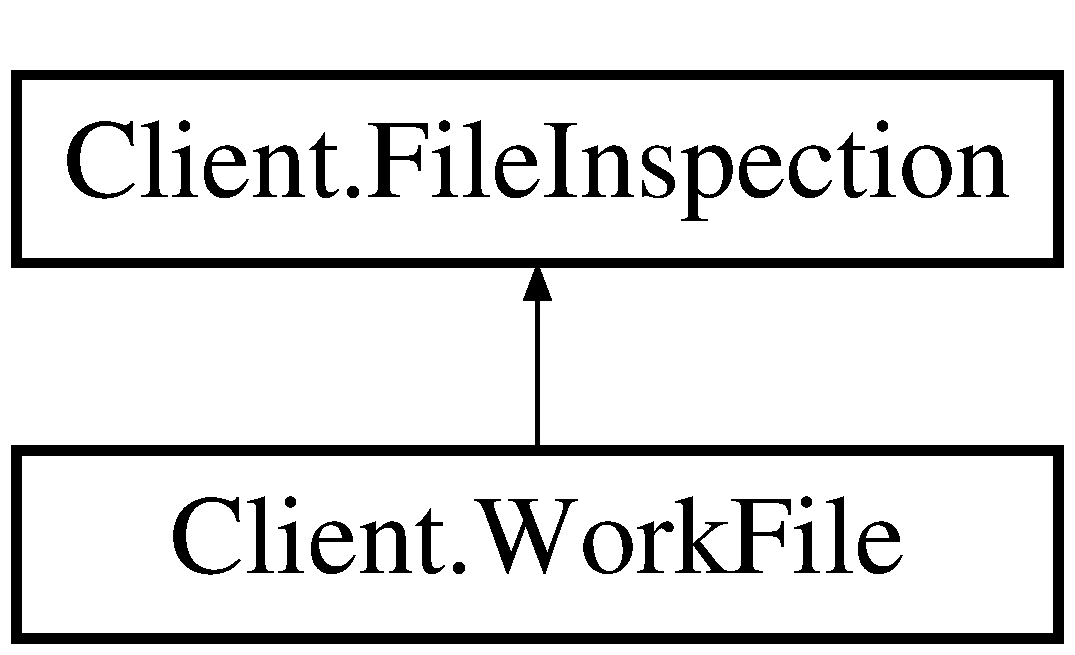
\includegraphics[height=2.000000cm]{class_client_1_1_work_file}
\end{center}
\end{figure}
\subsection*{Public Member Functions}
\begin{DoxyCompactItemize}
\item 
bool \hyperlink{class_client_1_1_work_file_a2133a018059220ccb5eca90ea39f0f72}{Create\+File} (string path\+File)
\begin{DoxyCompactList}\small\item\em Метод для создания файла + \end{DoxyCompactList}\item 
void \hyperlink{class_client_1_1_work_file_a1a78c0750e5d9e3f6e47f2a18d73ad14}{Create\+File} (string path\+File, string text)
\begin{DoxyCompactList}\small\item\em Метод для создания файла + \end{DoxyCompactList}\item 
int \hyperlink{class_client_1_1_work_file_aa6be3320b601af43b26ad4ad964cdc4f}{Get\+Posl\+Time} (int posl\+Time, string path\+File)
\begin{DoxyCompactList}\small\item\em Метод для поиска последнего времени в файле \end{DoxyCompactList}\item 
string \hyperlink{class_client_1_1_work_file_ac8d171e560e68dc71132752679d3387e}{Read\+File} (string path\+File)
\begin{DoxyCompactList}\small\item\em Функция для прочтения файла + \end{DoxyCompactList}\item 
List$<$ int $>$ \hyperlink{class_client_1_1_work_file_a98c27a5faa8b82ec7f64c9368d54c19a}{read} (string text\+Data\+Quote, List$<$ double $>$ mass\+Y\+Inet\+Buy, List$<$ double $>$ mass\+Y\+Inet\+Sell)
\begin{DoxyCompactList}\small\item\em Метод для парсинга данных и добавление значений в массив из файла \end{DoxyCompactList}\end{DoxyCompactItemize}
\subsection*{Additional Inherited Members}


\subsection{Detailed Description}
Класс отвечающий за работу с файлами 



\subsection{Member Function Documentation}
\hypertarget{class_client_1_1_work_file_a2133a018059220ccb5eca90ea39f0f72}{}\label{class_client_1_1_work_file_a2133a018059220ccb5eca90ea39f0f72} 
\index{Client\+::\+Work\+File@{Client\+::\+Work\+File}!Create\+File@{Create\+File}}
\index{Create\+File@{Create\+File}!Client\+::\+Work\+File@{Client\+::\+Work\+File}}
\subsubsection{\texorpdfstring{Create\+File()}{CreateFile()}\hspace{0.1cm}{\footnotesize\ttfamily [1/2]}}
{\footnotesize\ttfamily bool Client.\+Work\+File.\+Create\+File (\begin{DoxyParamCaption}\item[{string}]{path\+File }\end{DoxyParamCaption})\hspace{0.3cm}{\ttfamily [inline]}}



Метод для создания файла + 


\begin{DoxyParams}{Parameters}
{\em path\+File} & Путь к файлу \\
\hline
\end{DoxyParams}
\hypertarget{class_client_1_1_work_file_a1a78c0750e5d9e3f6e47f2a18d73ad14}{}\label{class_client_1_1_work_file_a1a78c0750e5d9e3f6e47f2a18d73ad14} 
\index{Client\+::\+Work\+File@{Client\+::\+Work\+File}!Create\+File@{Create\+File}}
\index{Create\+File@{Create\+File}!Client\+::\+Work\+File@{Client\+::\+Work\+File}}
\subsubsection{\texorpdfstring{Create\+File()}{CreateFile()}\hspace{0.1cm}{\footnotesize\ttfamily [2/2]}}
{\footnotesize\ttfamily void Client.\+Work\+File.\+Create\+File (\begin{DoxyParamCaption}\item[{string}]{path\+File,  }\item[{string}]{text }\end{DoxyParamCaption})\hspace{0.3cm}{\ttfamily [inline]}}



Метод для создания файла + 


\begin{DoxyParams}{Parameters}
{\em path\+File} & Путь к файлу \\
\hline
\end{DoxyParams}
\hypertarget{class_client_1_1_work_file_aa6be3320b601af43b26ad4ad964cdc4f}{}\label{class_client_1_1_work_file_aa6be3320b601af43b26ad4ad964cdc4f} 
\index{Client\+::\+Work\+File@{Client\+::\+Work\+File}!Get\+Posl\+Time@{Get\+Posl\+Time}}
\index{Get\+Posl\+Time@{Get\+Posl\+Time}!Client\+::\+Work\+File@{Client\+::\+Work\+File}}
\subsubsection{\texorpdfstring{Get\+Posl\+Time()}{GetPoslTime()}}
{\footnotesize\ttfamily int Client.\+Work\+File.\+Get\+Posl\+Time (\begin{DoxyParamCaption}\item[{int}]{posl\+Time,  }\item[{string}]{path\+File }\end{DoxyParamCaption})\hspace{0.3cm}{\ttfamily [inline]}}



Метод для поиска последнего времени в файле 


\begin{DoxyParams}{Parameters}
{\em posl\+Time} & Текущее последнее значение времени\\
\hline
{\em path\+File} & Путь к файлу \\
\hline
\end{DoxyParams}
\begin{DoxyReturn}{Returns}
Возвращение последнее значение времени
\end{DoxyReturn}
\hypertarget{class_client_1_1_work_file_a98c27a5faa8b82ec7f64c9368d54c19a}{}\label{class_client_1_1_work_file_a98c27a5faa8b82ec7f64c9368d54c19a} 
\index{Client\+::\+Work\+File@{Client\+::\+Work\+File}!read@{read}}
\index{read@{read}!Client\+::\+Work\+File@{Client\+::\+Work\+File}}
\subsubsection{\texorpdfstring{read()}{read()}}
{\footnotesize\ttfamily List$<$int$>$ Client.\+Work\+File.\+read (\begin{DoxyParamCaption}\item[{string}]{text\+Data\+Quote,  }\item[{List$<$ double $>$}]{mass\+Y\+Inet\+Buy,  }\item[{List$<$ double $>$}]{mass\+Y\+Inet\+Sell }\end{DoxyParamCaption})\hspace{0.3cm}{\ttfamily [inline]}}



Метод для парсинга данных и добавление значений в массив из файла 


\begin{DoxyParams}{Parameters}
{\em text\+Data\+Quote} & Строка с триадами\\
\hline
{\em mass\+Y\+Inet\+Buy} & Массив значений покупок\\
\hline
{\em mass\+Y\+Inet\+Sell} & Массив значений продажи\\
\hline
{\em Times} & Массив звремени\\
\hline
\end{DoxyParams}
\begin{DoxyReturn}{Returns}
Возвращение кол-\/ва записей из стринга
\end{DoxyReturn}
\hypertarget{class_client_1_1_work_file_ac8d171e560e68dc71132752679d3387e}{}\label{class_client_1_1_work_file_ac8d171e560e68dc71132752679d3387e} 
\index{Client\+::\+Work\+File@{Client\+::\+Work\+File}!Read\+File@{Read\+File}}
\index{Read\+File@{Read\+File}!Client\+::\+Work\+File@{Client\+::\+Work\+File}}
\subsubsection{\texorpdfstring{Read\+File()}{ReadFile()}}
{\footnotesize\ttfamily string Client.\+Work\+File.\+Read\+File (\begin{DoxyParamCaption}\item[{string}]{path\+File }\end{DoxyParamCaption})\hspace{0.3cm}{\ttfamily [inline]}}



Функция для прочтения файла + 

\begin{DoxyReturn}{Returns}
Текст прочтенного из файла
\end{DoxyReturn}


The documentation for this class was generated from the following file\+:\begin{DoxyCompactItemize}
\item 
C\+:/\+Users/саша/\+Documents/\+Visual Studio 2015/\+Projects/\+Forex2.\+0/\+Client/Work\+File.\+cs\end{DoxyCompactItemize}

\hypertarget{class_client_1_1_zoom_s}{}\section{Client.\+ZoomS Class Reference}
\label{class_client_1_1_zoom_s}\index{Client.\+ZoomS@{Client.\+ZoomS}}


Класс для работы с масштабоом графика  


\subsection*{Public Member Functions}
\begin{DoxyCompactItemize}
\item 
\hyperlink{class_client_1_1_zoom_s_acb727e42e42338ff7d2381368cdf8645}{ZoomS} (List$<$ int $>$ a, int Period)
\begin{DoxyCompactList}\small\item\em Измененение маштаба \end{DoxyCompactList}\end{DoxyCompactItemize}
\subsection*{Public Attributes}
\begin{DoxyCompactItemize}
\item 
int \hyperlink{class_client_1_1_zoom_s_aa616e068719d96465c5807c6c1b50eac}{start}
\begin{DoxyCompactList}\small\item\em Стартовое время \end{DoxyCompactList}\item 
int \hyperlink{class_client_1_1_zoom_s_a27e81af9efa762e3a2cc24833111a232}{end}
\begin{DoxyCompactList}\small\item\em конечное время \end{DoxyCompactList}\item 
List$<$ int $>$ \hyperlink{class_client_1_1_zoom_s_a86111434f20994bf245105ff9378e3bb}{New\+Zoom} = new List$<$int$>$()
\begin{DoxyCompactList}\small\item\em Новый лист времени \end{DoxyCompactList}\item 
\hypertarget{class_client_1_1_zoom_s_ac0bceac7fb7c576784c6d5a788e32aec}{}\label{class_client_1_1_zoom_s_ac0bceac7fb7c576784c6d5a788e32aec} 
List$<$ int $>$ {\bfseries Zoom} = new List$<$int$>$()
\end{DoxyCompactItemize}


\subsection{Detailed Description}
Класс для работы с масштабоом графика 



\subsection{Constructor \& Destructor Documentation}
\hypertarget{class_client_1_1_zoom_s_acb727e42e42338ff7d2381368cdf8645}{}\label{class_client_1_1_zoom_s_acb727e42e42338ff7d2381368cdf8645} 
\index{Client\+::\+ZoomS@{Client\+::\+ZoomS}!ZoomS@{ZoomS}}
\index{ZoomS@{ZoomS}!Client\+::\+ZoomS@{Client\+::\+ZoomS}}
\subsubsection{\texorpdfstring{Zoom\+S()}{ZoomS()}}
{\footnotesize\ttfamily Client.\+Zoom\+S.\+ZoomS (\begin{DoxyParamCaption}\item[{List$<$ int $>$}]{a,  }\item[{int}]{Period }\end{DoxyParamCaption})\hspace{0.3cm}{\ttfamily [inline]}}



Измененение маштаба 



\subsection{Member Data Documentation}
\hypertarget{class_client_1_1_zoom_s_a27e81af9efa762e3a2cc24833111a232}{}\label{class_client_1_1_zoom_s_a27e81af9efa762e3a2cc24833111a232} 
\index{Client\+::\+ZoomS@{Client\+::\+ZoomS}!end@{end}}
\index{end@{end}!Client\+::\+ZoomS@{Client\+::\+ZoomS}}
\subsubsection{\texorpdfstring{end}{end}}
{\footnotesize\ttfamily int Client.\+Zoom\+S.\+end}



конечное время 

\hypertarget{class_client_1_1_zoom_s_a86111434f20994bf245105ff9378e3bb}{}\label{class_client_1_1_zoom_s_a86111434f20994bf245105ff9378e3bb} 
\index{Client\+::\+ZoomS@{Client\+::\+ZoomS}!New\+Zoom@{New\+Zoom}}
\index{New\+Zoom@{New\+Zoom}!Client\+::\+ZoomS@{Client\+::\+ZoomS}}
\subsubsection{\texorpdfstring{New\+Zoom}{NewZoom}}
{\footnotesize\ttfamily List$<$int$>$ Client.\+Zoom\+S.\+New\+Zoom = new List$<$int$>$()}



Новый лист времени 

\hypertarget{class_client_1_1_zoom_s_aa616e068719d96465c5807c6c1b50eac}{}\label{class_client_1_1_zoom_s_aa616e068719d96465c5807c6c1b50eac} 
\index{Client\+::\+ZoomS@{Client\+::\+ZoomS}!start@{start}}
\index{start@{start}!Client\+::\+ZoomS@{Client\+::\+ZoomS}}
\subsubsection{\texorpdfstring{start}{start}}
{\footnotesize\ttfamily int Client.\+Zoom\+S.\+start}



Стартовое время 



The documentation for this class was generated from the following file\+:\begin{DoxyCompactItemize}
\item 
C\+:/\+Users/саша/\+Documents/\+Visual Studio 2015/\+Projects/\+Forex2.\+0/\+Client/Zoom\+S.\+cs\end{DoxyCompactItemize}

%--- End generated contents ---

% Index
\backmatter
\newpage
\phantomsection
\clearemptydoublepage
\addcontentsline{toc}{chapter}{Index}
\printindex

\end{document}
